\documentclass[12pt]{article}

\usepackage[margin=50pt]{geometry}
\usepackage{amsmath}
\usepackage{amssymb}
\usepackage{graphicx}
\usepackage{hyperref}
\usepackage{caption}
\usepackage{subcaption}
\usepackage{multirow}
\usepackage{pdfpages}

\DeclareMathOperator*{\argmax}{arg\,max}
\DeclareMathOperator*{\argmin}{arg\,min}

\graphicspath{/images}
\geometry{footskip=0.8cm}

\title{Data Mining}
\author{Thomas Vroom}

\begin{document}
\maketitle

\tableofcontents

%
% Topic 1 - Introduction to Data Mining
%
\newpage
\section{Introduction to Data Mining}
The last couple of decades has seen a huge flood in the amount of data that needs to be processed.
As database management systems become capable of handling bigger and bigger databases, and storage technology becomes faster and cheaper, the \textbf{Storage Law} states that the total amount of data stored in the world \textit{doubles} roughly every 9 months.
Comparing this to \textbf{Moore's law}, which states that the speed of computers doubles roughly every 18 months, we can see that data is stored much faster than it can be processed!
Very little data will ever be looked at by a human, which means we need to automate the process of \textbf{Knowledge Discovery} to make sense and use of data.

\subsection{Knowledge Discovery}
Knowledge discovery from data is a non-trivial process of identifying \textbf{Valid}, \textbf{Novel}, potentially \textbf{Useful}, and ultimately \textbf{Understandable Patterns} in data.
It is a field closely related to \textit{Machine Learning} (the study of computer algorithms that improve automatically through experience), \textit{Statistics} (the mathematical science pertaining to the collection, analysis, interpretation or exploration of data), \textit{Visualization} (the study of techniques for creating images, diagrams, or animations to communicate a message), and \textit{Databases} (a scientific discipline that studies how data has to be represented, structured and managed on computers).

\begin{figure}[h]
    \centering
    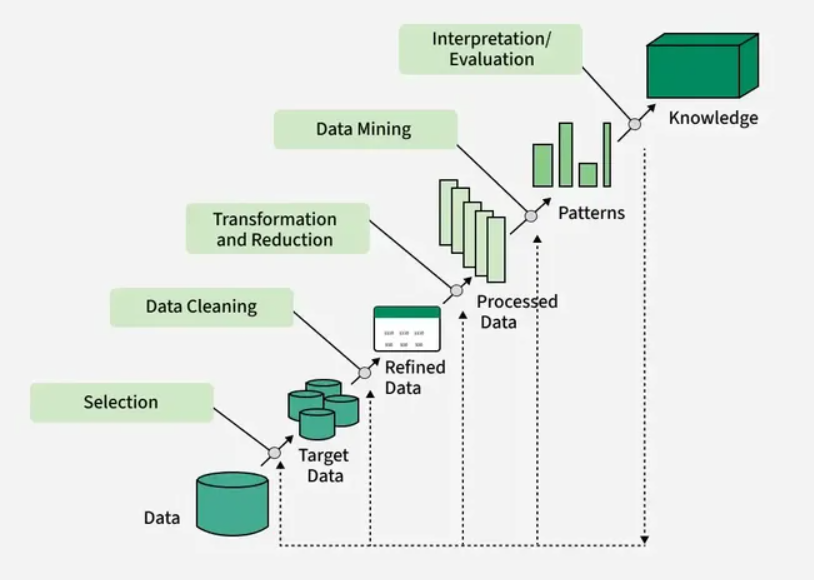
\includegraphics[scale=0.75]{images/knowledge-discovery.PNG}
    \caption{A diagram of the \textit{Knowledge Discovery Process}. \textbf{(1) Selection:} the process of gathering data to form a raw dataset. \textbf{(2) Data Cleaning / Preprocessing:} ensuring that the dataset is of good quality by e.g. handling missing values, inconsistencies, noise, etc. \textbf{(3) Transformation and Feature Selection:} selecting or generating informative features. \textbf{(4) Data Mining:} searching for patterns of interest in a particular representation. \textbf{(5) Interpretation and Validation:} giving meaning to the results and verifying that what we have learned is correct / informative.}
\end{figure}

\newpage
\subsection{Data Mining Tasks}
Data Mining can often be subdivided into the following four tasks: \textbf{Classification}, \textbf{Regression}, \textbf{Clustering}, and \textbf{Association-Rule Mining}.

\noindent
\\
In a \textbf{Classification} task we are given an instance space $X$ and a \textit{discrete} variable $Y$, with the goal of finding the most probable classification $y \in Y$ for a new instance $x \in X$. Note that the number of instances in the training data must be larger than the number of variables in the instance space (if you have more variables than instances you can explain everything).

\begin{figure}[h]
    \centering
    \begin{subfigure}{.5\textwidth}
        \centering
        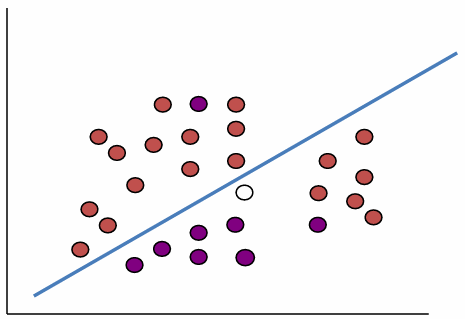
\includegraphics[width=.8\linewidth]{images/classification1.PNG}
        \caption{A linear classifier.\label{fig:classification-linear}}
    \end{subfigure}%
    \begin{subfigure}{.5\textwidth}
        \centering
        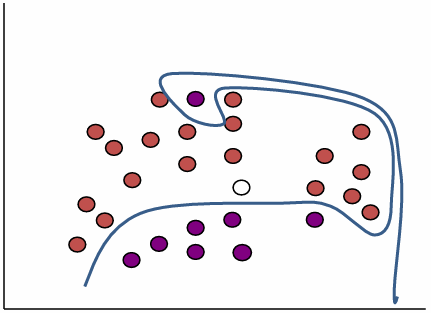
\includegraphics[width=.8\linewidth]{images/classification2.PNG}
        \caption{A non-linear classifier.\label{fig:classification-non-linear}}
    \end{subfigure}
\caption{An example of classification. The blue line is called a \textbf{Classifier} / \textbf{Hypothesis} / \textbf{Decision Boundary}. \ref{fig:classification-linear} shows a linear classifier that is likely \textbf{Underfitted} (it is not using the data to its full potential). Note that an underfitted model is not necessarily suboptimal: if the data in this example is very noisy, then this classifier could be optimal. \ref{fig:classification-non-linear} shows a non-linear classifier that is likely \textbf{Overfitted} (it is so tuned on the training data that it loses generalization).}
\end{figure}

\begin{figure}[h]
    \centering
    \begin{subfigure}{.5\textwidth}
        \centering
        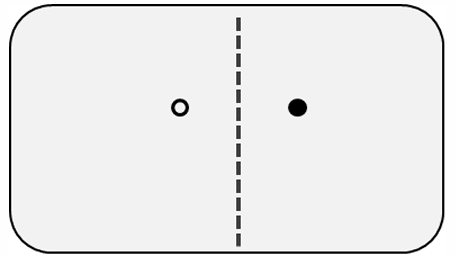
\includegraphics[width=.8\linewidth]{images/unlabeled-data1.PNG}
        \caption{A linear decision boundary.\label{fig:unlabeled-data1}}
    \end{subfigure}%
    \begin{subfigure}{.5\textwidth}
        \centering
        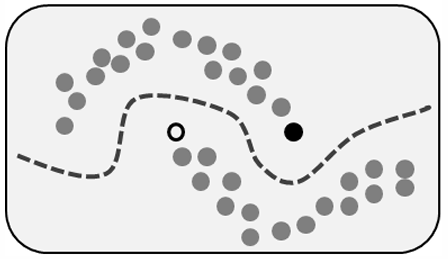
\includegraphics[width=.8\linewidth]{images/unlabeled-data2.PNG}
        \caption{A non-linear decision boundary.\label{fig:unlabeled-data2}}
    \end{subfigure}
\caption{\textbf{Can unlabeled data be helpful?} \ref{fig:unlabeled-data1} shows only two labeled data points with a linear decision boundary between them. With no further information given, we can say that this decision boundary is optimal. \ref{fig:unlabeled-data2} shows the same dataset, but this time including all the unlabeled data. Now it is suddenly clear that we should not use a linear decision boundary for this problem.}
\end{figure}

\noindent
Data points close to or on the decision boundary are the most informative.
A common strategy for when data labeling is tedious or expensive is \textbf{Active Learning}: train a model using the available data, generate new instances close to the model's decision boundary, label those instances manually, add these new instances to the training data, and repeat.

\newpage
\noindent
In a \textbf{Regression} task we are given an instance space $X$ and a \textit{continuous} variable $Y$, with the goal of finding the most probable value $y \in Y$ for a new instance $x \in X$.

\begin{figure}[h!]
    \centering
    \begin{subfigure}{.5\textwidth}
        \centering
        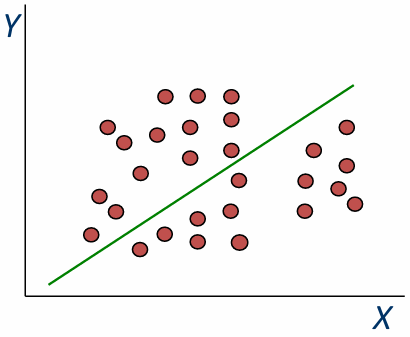
\includegraphics[width=.8\linewidth]{images/regression1.PNG}
        \caption{A linear regressor.\label{fig:regression-linear}}
    \end{subfigure}%
    \begin{subfigure}{.5\textwidth}
        \centering
        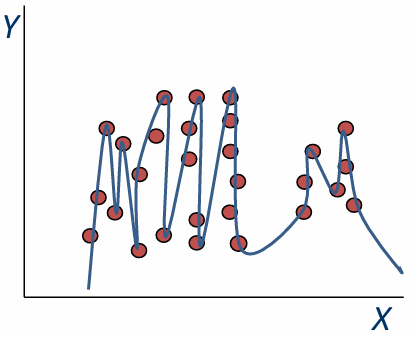
\includegraphics[width=.8\linewidth]{images/regression2.PNG}
        \caption{A non-linear regressor.\label{fig:regression-non-linear}}
    \end{subfigure}
\caption{An example of regression.}
\end{figure}

\noindent
In a \textbf{Clustering} task we are given an instance space $X$ and a bunch of training data sampled from $X$, with the goal of finding clusters such that instances within each cluster are more similar and instances in separate clusters are less similar.
Clustering is an example of \textbf{Unsupervised Learning}, as we do not have any labels for the data.

\begin{figure}[h]
    \centering
    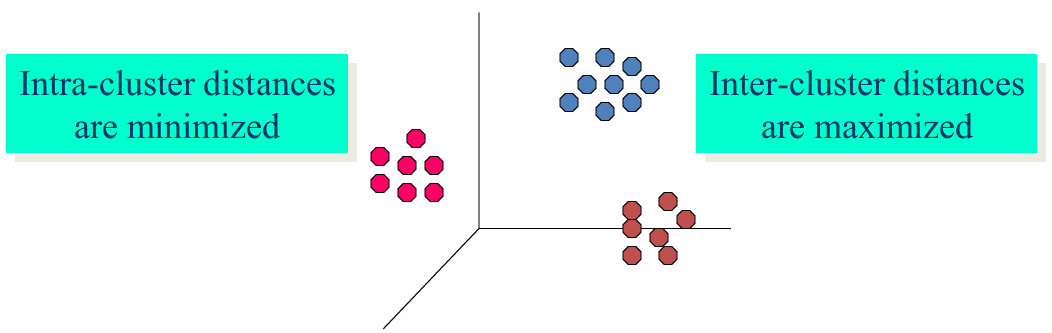
\includegraphics[scale=0.8]{images/clustering.PNG}
    \caption{An example of clustering.\label{fig:cluster}}
\end{figure}

\noindent
An important concept for data mining is \textbf{Inductive Bias}:
Assume we have an infinite instance space $X$ where instances can be labeled one of two classes.
Additionally, we have an unrestricted (unbiased) hypothesis space $H$ (i.e. $h \in H$ could take on any possible decision boundary), and we have an unrestricted (unbiased) search algorithm that finds all classifiers $h \in H$ that are consistent with the data.
In this case the search algorithm will find for \textit{any} set of training data an \textit{infinite} amount of classifiers $h$, such that for any new test instance $x$ half of the classifiers will classify $x$ as one class while the other half will classify $x$ as the other class.
If we want to classify \textit{beyond} the training data, we need to restrict (bias) either the hypothesis space $H$ (\textbf{Representation Inductive Bias}) or the search algorithm (\textbf{Search Inductive Bias}).
Practically we prefer the latter, since it guarantees that the theoretical optimal classifier $h$ is in the hypothesis space $H$ (there is a possibility we find it).

\newpage
\noindent
In a \textbf{Association-Rule Mining} task we are given a set of records, each of which contain some number of items from a given collection.
The goal is to produce dependency rules that predict the occurrence of an item based on the occurrences of other items.

\begin{figure}[h]
    \centering
    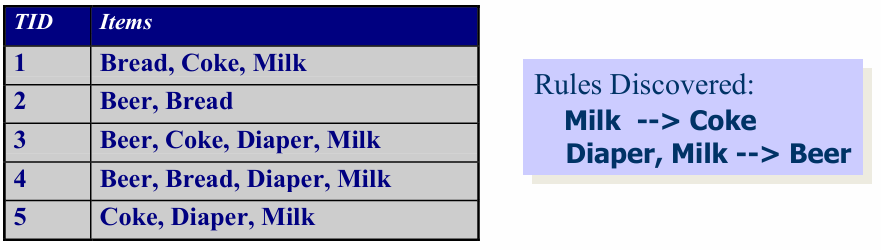
\includegraphics[scale=0.8]{images/association-rule.PNG}
    \caption{An example of an Association-Rule Mining task. The result of this example would be to put these products closer to each other in the store. Another example of Association-Rule Mining is in medical science, where the task is to find out which diseases lead to other diseases over time.\label{fig:association-rule-mining}}
\end{figure}

\subsection{Defining Data}
Datasets are made up of \textbf{Data Objects}: a representation of an object of interest (also known as records, points, cases, samples, entities, or instances).
Data objects are described by \textbf{Variables}: a representation of a property or characteristic of an object (also known as field, characteristic, or feature).
A variable $V$ is a tuple $<Name, Domain, Operations, Scale>$, where: $Name$ is the name of $V$, $Domain$ is the set of values for $V$, $Operations$ is the set of operations allowed over $Domain$, and $Scale$ is a rule that associates a value from $Domain$ for the variable $V$ when it represents an object $o$.

\begin{table}[h]
    \centering
    \begin{tabular}{ccc}
    Variable Type & Operations & Transformations \\ \hline
    \textbf{Nominal Variables} & $=, \neq$ & Any permutation of values \\
    \textbf{Ordinal Variables} & $=, \neq, <, >$ & $x_2 = f(x_1)$, where $f$ is order-preserving \\
    \textbf{Interval-Scaled Variables} & $=, \neq, <, >, +, -$ & $x_2 = a \cdot x_1 + b$ \\
    \textbf{Ratio-Scaled Variables} & $=, \neq, <, >, +, -, \cdot, /$ & $x_2 = a \cdot x_1$
    \end{tabular}
    \caption{Different types of variables. \textbf{Nominal Variables} are variables whose values are symbols (e.g. zip codes, employee IDs, eye color, etc.), if a Nominal variable only has two values then it is also called a \textbf{Binary Variable}. \textbf{Ordinal Variables} are variables whose values can be ordered (e.g. grades, street numbers, etc.), Nominal and Ordinal variables are both \textbf{Discrete}. \textbf{Interval-Scaled Variables} are measured on a scale of equal-size units, but without a natural zero point (e.g. calendar dates, temperature in $C$ \textit{(if yesterday was $10^\circ C$ and today is $20^\circ C$, then today is not twice as hot as yesterday)}, etc.), and \textbf{Ratio-Scaled Variables} are variables that do have an inherent zero point (e.g. temperature in $K$, counts, age, weight, length, etc.). Interval-Scaled and Ratio-Scaled variables are both \textbf{Continuous}.}
\end{table}

\noindent
Variables can either be \textbf{Symmetric} (all outcomes are equally important, e.g. gender) or \textbf{Asymmetric} (not all outcomes are equally important, e.g. medical test).
For asymmetric variables, standard distance measures (e.g. euclidean distance) do not work!

\newpage
\noindent
Data can also be categorized in the following types:

\begin{itemize}
    \item \textbf{Record-based Data}: data that consists of a collection of records, each of which is represented by a set of variables that can be constant or varying from record to record. If data objects have the same fixed set of numeric variables, then the objects can be represented as a \textbf{Data Matrix}. In \textbf{Document Data} the value of a variable, called \textit{term} in this context, is the number of times that term occurs in the document. In \textbf{Transaction Data} each record involves a different set of variables (e.g. a grocery receipt).
    \item \textbf{Graph-based Data}: data stored in a graph (e.g. social networks, molecule structures, etc.).
    \item \textbf{Ordered Data}: data with an inherent ordering (e.g. genome sequences, etc.).
\end{itemize}

\noindent
Important characteristics of data are the \textbf{Dimensionality} (how many variables have been used?), \textbf{Sparsity} (how many asymmetric variables have been used? Note that as sparsity increases, the usefulness of distance measures decrease: not many instances have the sparse variables, so all the data is close to each other), and \textbf{Resolution} (how many variables have been aggregated?).

\begin{figure}[h]
    \centering
    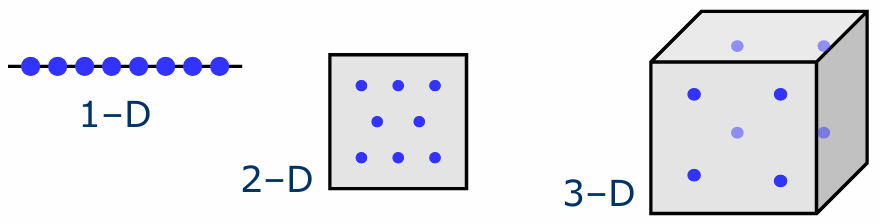
\includegraphics[scale=0.8]{images/curse-of-dimensionality.PNG}
    \caption{Data mining problems are often massive in both the number of instances as well as the number of dimensions. This can lead to problems such as the \textbf{Curse of Dimensionality}: as dimensions increase, data needs to exponentially increase to keep the same density. In the above example eight points almost completely cover a 1D-space, but become more and more separated as the dimensions increase. A rule of thumb is that for every variable you add, you would need to \textit{double} the data to keep the same density. In practice, the usual solution for this is \textbf{Feature Selection}.}
\end{figure}

\subsection{Statistical Properties of Data}

\begin{table}[h!]
    \centering
    \begin{tabular}{c|c}
    Operation & Formula \\ \hline
    \textbf{Population Mean} & $\mu = \displaystyle\frac{\sum x}{N}$ \\
    \textbf{Sample Mean} & $\bar{x} = \displaystyle\frac{1}{n} \sum_{i = 1}^n x_i$ \\
    \textbf{Weighted Arithmetic Mean} & $\bar{x} = \displaystyle\frac{\sum_{i = 1}^n w_i x_i}{\sum_{i = 1}^n w_i}$ \\
    \textbf{Median} & $\begin{cases}\text{The middle value,} & \text{ if } n = \text{odd} \\ \text{The average of the middle values,} & \text{ if } n = \text{even}\end{cases}$ \\
    \textbf{Mode} & The value that occurs most frequently
    \end{tabular}
\end{table}

\newpage

\begin{figure}[h]
    \centering
    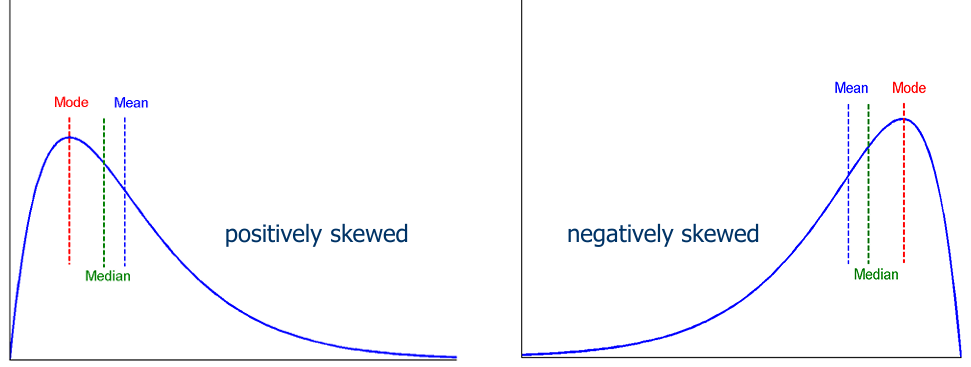
\includegraphics[scale=0.8]{images/skewed-data.PNG}
    \caption{Data can either be \textbf{Symmetric} (in which case mean, median and mode overlap), \textbf{Positively Skewed}, or \textbf{Negatively Skewed}. If data is moderately skewed, then mean, median and mode can be related through the \textit{approximate} formula: $mean - mode = 3(mean - median)$.}
\end{figure}

\noindent
Given a set of values $x_1, x_2, ..., x_n$ for a numeric variable $X$, the \textbf{Range} of the set is the difference between the minimal and maximal elements in the set.
The $k$th $q$-\textbf{Quantile} is the value $x$ such that at most $\displaystyle\frac{nk}{q}$ values will be smaller than $x$ and at most $\displaystyle\frac{n(q - k)}{q}$ values will be greater than $x$.
The index of the $k$th $q$-quantile can be computed as $\displaystyle\frac{nk}{q}$.
If the result is not an integer, then round up to the next integer.
Common instances of quantiles are \textbf{Quartiles} ($q = 4$) and \textbf{Percentiles} ($q = 100$).
The \textbf{Inter-Quartile Range (IQR)} provides a measure of statistical dispersion, showing how much the data is spread around the \textit{median}. Usually, any data point more than $1.5 \cdot IQR$ below $Q_1$ or above $Q_3$ can be considered an outlier.

\begin{figure}[h]
    \centering
    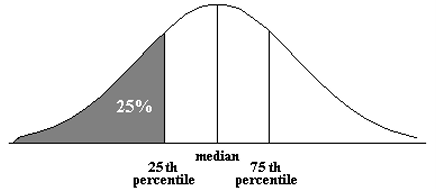
\includegraphics{images/IQR.PNG}
    \caption{$IQR = Q_3 - Q_1$}
\end{figure}

\noindent
The \textbf{Population Variance} ($Var(X)$ or $\sigma^2$) can be calculated using the following formula:
\[ \sigma^2 = \frac{1}{N} \sum_{i = 1}^N \left( x_i - \mu \right)^2 \]

\noindent
Note that for a small subset of a larger population, the \textbf{Sample Variance} should be used instead:
\[ s^2 = \frac{1}{n - 1} \sum_{i = 1}^n \left( x_i - \bar{x} \right)^2 \]

\noindent
The \textbf{Standard Deviation} is the square root of the variance.

\newpage
\begin{figure}[h]
    \centering
    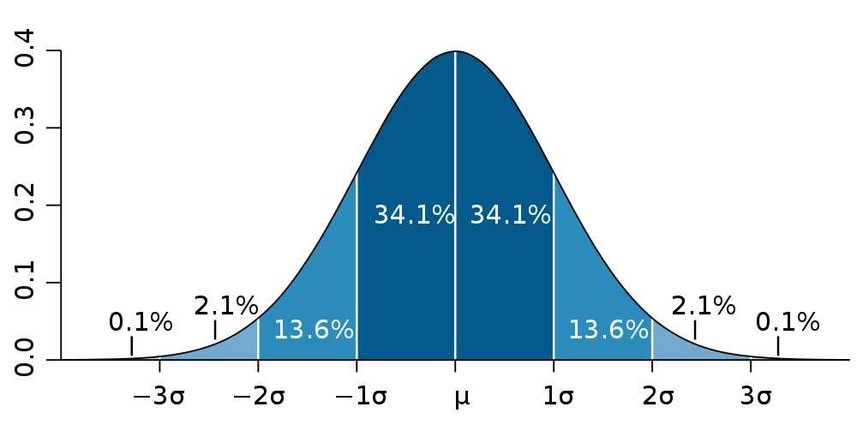
\includegraphics[scale=0.5]{images/normal-distribution.jpg}
    \caption{An example of a \textbf{Normal Distribution}. From $\mu - \sigma$ to $\mu + \sigma$ contains about 68\% of all measurements. From $\mu - 2\sigma$ to $\mu + 2\sigma$ contains about 95\%, and from $\mu - 3\sigma$ to $\mu + 3\sigma$ contains about 99.7\%.}
\end{figure}

\begin{table}[h]
    \centering
    \begin{tabular}{c|c}
    Variable Type & (Statistical) Operations \\ \hline
    \textbf{Nominal Variables} & mode \\
    \textbf{Ordinal Variables} & median, percentiles, + all above \\
    \textbf{Interval-Scaled Variables} & mean, standard deviation, + all above \\
    \textbf{Ratio-Scaled Variables} & geometric mean, harmonic mean, + all above
    \end{tabular}
    \caption{The statistical properties allowed over different variable types. The \textbf{Geometric Mean} is more appropriate for numbers that are multiplicative, e.g. percentages: $GM = \displaystyle\sqrt[n]{x_1 \cdot x_2 \cdot ... \cdot x_n}$. The \textbf{Harmonic Mean} is more appropriate for ratios and rates, e.g. speeds, and is ideally only used with positive arguments: $HM = \left(\displaystyle\frac{1}{n}\sum_{i = 1}^n x_i^{-1}\right)^{-1}$.}
\end{table}

\subsection{Visualization}
\begin{figure}[h!]
    \centering
    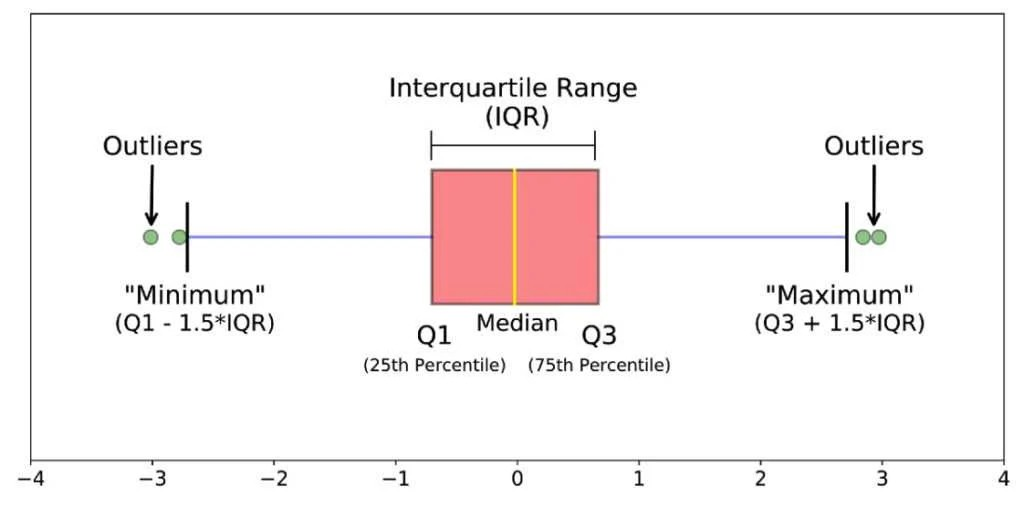
\includegraphics[scale=0.35]{images/boxplot.png}
    \caption{A \textbf{Boxplot} shows a five-number summary of a distribution. Boxplots are great for identifying outliers, comparing datasets side-by-side, and understanding the spread of a dataset.}
\end{figure}

\newpage
\begin{figure}[h]
    \centering
    \begin{subfigure}{.5\textwidth}
        \centering
        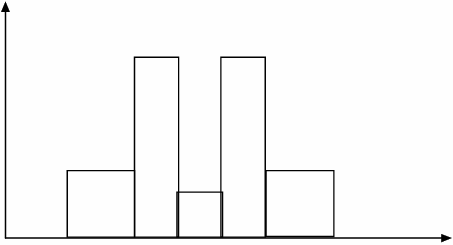
\includegraphics[width=0.95\linewidth]{images/histogram1.PNG}
        \caption{\label{fig:histogram1}}
    \end{subfigure}%
    \begin{subfigure}{.5\textwidth}
        \centering
        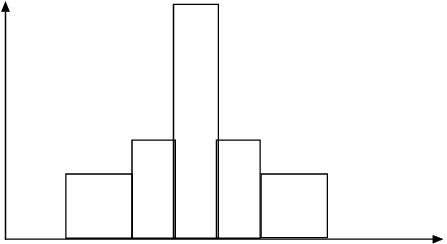
\includegraphics[width=0.95\linewidth]{images/histogram2.PNG}
        \caption{\label{fig:histogram2}}
    \end{subfigure}
\caption{\textbf{Histograms} are $x, y$ diagrams such that the $x$-axis represents possible values and the $y$-axis represents their frequencies. They usually show the distribution of values for a single variable, but can be adapted to 3D to show the joint distribution of values for two variables. For continuous variables the range is split into a set of bins, and a barplot is used to show the number of objects in each bin. Histograms often tell us more than boxplots: The two histograms shown in \ref{fig:histogram1} and \ref{fig:histogram2} have the same boxplot representation, but have rather different data distributions. Histograms are the preferred visualization type for \textit{ordinal} variables.}
\end{figure}

\begin{figure}[h!]
    \centering
    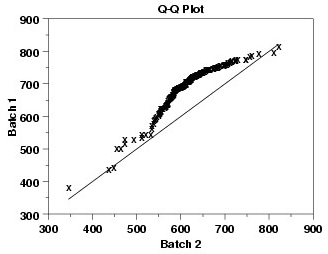
\includegraphics{images/q-q-plot.png}
    \caption{A \textbf{Quantile-Quantile (Q-Q) Plot} shows the quantiles of one univariate distribution against the corresponding quantiles of another. The more similar the distributions are, the more linear the line will be. In a Q-Q plot we can easily see if there is a shift in going from one distribution to another. In this example \textit{Batch 1} seems to have higher values than \textit{Batch 2}.}
\end{figure}

\newpage
\begin{figure}[h]
    \centering
    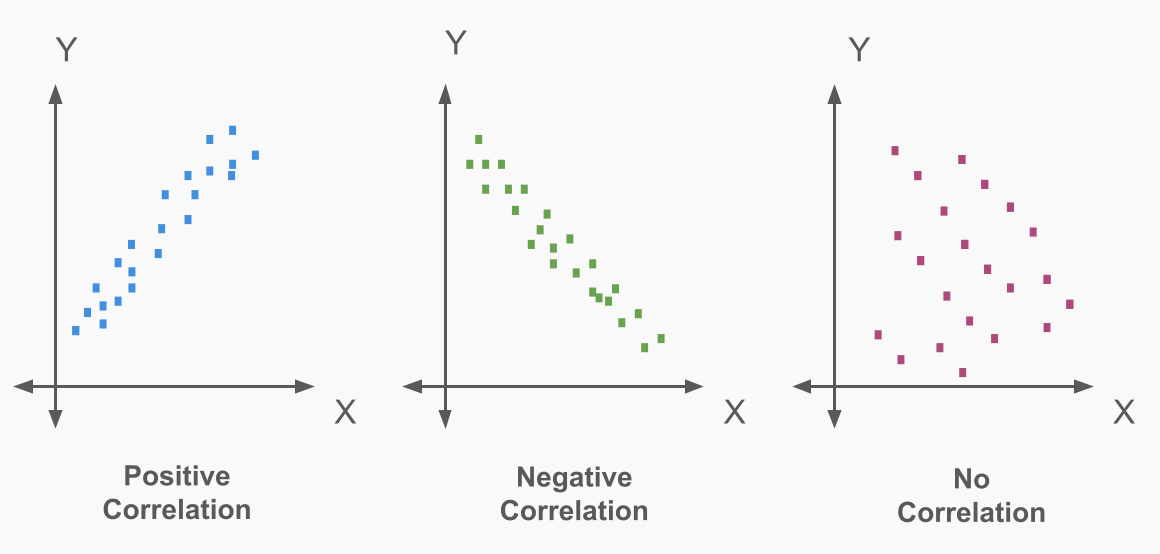
\includegraphics[scale=0.55]{images/scatter-plot.png}
    \caption{\textbf{Scatter Plots} represent objects as points in the plane given by pairs of values of two variables. These plots provide a first look at bivariate data to see clusters, outliers, etc. We can also empirically observe if data is positively or negatively correlated, or if there is no correlation at all.}
\end{figure}

\begin{figure}[h!]
    \centering
    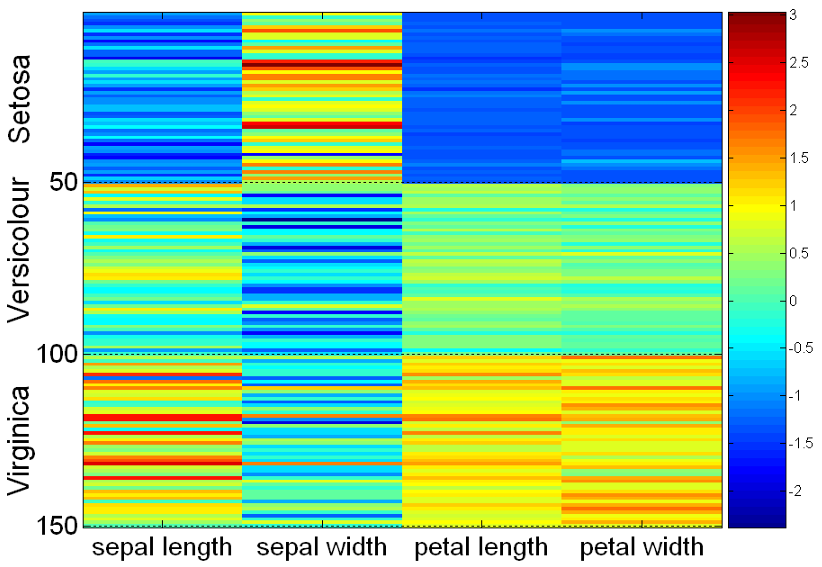
\includegraphics[scale=0.8]{images/pixel-visualization.PNG}
    \caption{\textbf{Pixel-Oriented Visualization Techniques} allow for the visualization of more than one or two variables. For a dataset of $m$ dimensions, create $m$ windows. The $m$ values of single record can then be mapped to $m$ pixels at corresponding positions in the windows, with their colors corresponding to their values.}
\end{figure}

\newpage
\begin{figure}[h]
    \centering
    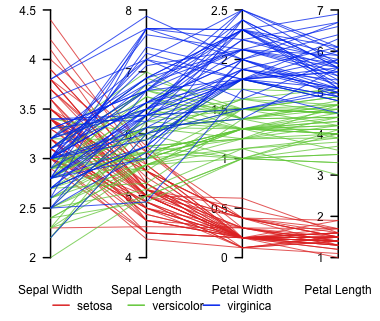
\includegraphics[scale=0.8]{images/parallel-coordinates.png}
    \caption{\textbf{Parallel Coordinates Plots} are a common method for visualizing high-dimensional datasets. $m$ equidistant axes are drawn parallel to one of the main axes and correspond to the $m$ variables. Each axis is scaled to the $[min, max]$ range of the corresponding variable. Each record corresponds to a polygonal line which intersects each of the axes at the point which corresponds to the value of the variable.}
\end{figure}

\begin{figure}[h]
    \centering
    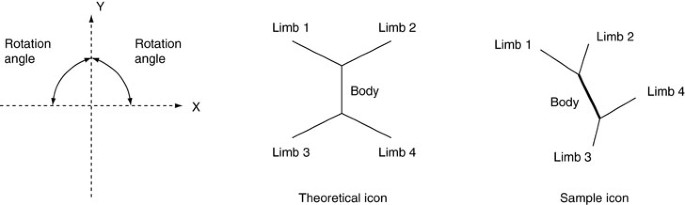
\includegraphics[scale=0.5]{images/stick-figures.jpg}
    \caption{\textbf{Icon-Based Visualization Techniques} visualize the data values as features of icons. Famous examples of this are \textit{Chernoff Faces} and \textit{Stick Figures}, which use shape to represent certain information.}
\end{figure}

\begin{figure}[h!]
    \centering
    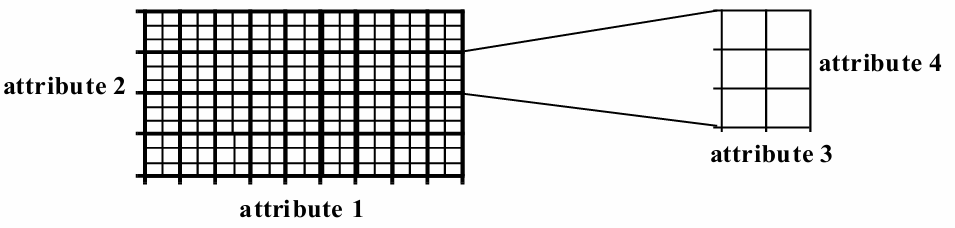
\includegraphics[scale=0.7]{images/dimensional-stacking.PNG}
    \caption{\textbf{Dimensional Stacking} is a popular \textbf{Hierarchical Visualization Technique}. It partitions an $m$-dimensional variable space into 2D subspaces, which are 'stacked into' each other (more important variables on the outer levels). In this example \textit{attribute 1} has 8, \textit{attribute 2} has 4, \textit{attribute 3} has 2, and \textit{attribute 4} has 3 possible values (or bins). This visualization is often adequate for data with ordinal variables of low cardinality, but it is difficult to display more than nine dimensions.}
\end{figure}

\newpage
\begin{figure}[h]
    \centering
    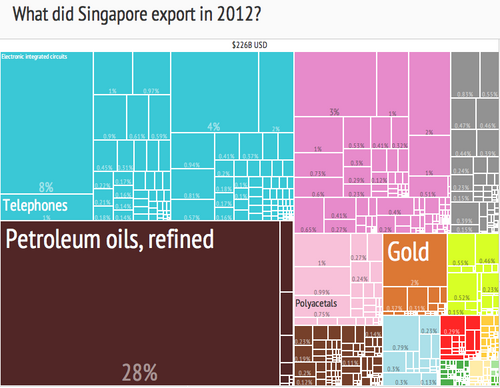
\includegraphics[scale=0.5]{images/treemap.png}
    \caption{A \textbf{Treemap} is another hierarchical visualization technique. Treemaps display tree-structured (hierarchical) data as a set of nested rectangles. Each branch of the tree is given a rectangle, which is then tiled with smaller rectangles representing sub-branches. A leaf node's rectangle has an area proportional to a specified dimension of the data. Often the leaf nodes are colored to show a separate dimension of the data. Treemaps make efficient use of space, and as a result can legibly display thousands of items on a screen simultaneously. Treemaps can also be used to display non-numerical data, such as text or social networks.}
\end{figure}

\subsection{Measuring Similarity}
\textbf{Similarity} is a numeric measure of how alike two data objects are. It often falls in the range $[0, 1]$, with higher values meaning the objects are more alike.
The opposite of similarity is \textbf{Dissimilarity} or \textbf{Distance}: a numeric measure of how far apart two data objects are.
Distance often falls in the range $[0, \infty]$, with lower values meaning the objects are more alike.
The term \textbf{Proximity} is often used in reference to either similarity or distance.

\noindent
\\
We can measure the proximity of \textit{binary} variables by constructing a \textbf{Contingency Table}:

\begin{table}[h]
    \centering
    \begin{tabular}{ccccc}
         & \multicolumn{4}{c}{Object $j$} \\ \cline{2-5} 
        \multicolumn{1}{c|}{\multirow{4}{*}{Object $i$}} & \multicolumn{1}{c|}{} & 1 & \multicolumn{1}{c|}{0} & \multicolumn{1}{c|}{$sum$} \\ \cline{2-5} 
        \multicolumn{1}{c|}{} & \multicolumn{1}{c|}{1} & $q$ & \multicolumn{1}{c|}{$r$} & \multicolumn{1}{c|}{$q+r$} \\
        \multicolumn{1}{c|}{} & \multicolumn{1}{c|}{0} & $s$ & \multicolumn{1}{c|}{$t$} & \multicolumn{1}{c|}{$s+t$} \\ \cline{2-5} 
        \multicolumn{1}{c|}{} & \multicolumn{1}{c|}{$sum$} & $q+s$ & \multicolumn{1}{c|}{$r+t$} & \multicolumn{1}{c|}{$p$} \\ \cline{2-5} 
    \end{tabular}
\end{table}

\noindent
From here, similarity and distance for \textit{symmetric} binary variables can be calculated as:
\begin{align*}
    sim(i, j) = \frac{q + t}{q + r + s + t} && d(i, j) = \frac{r + s}{q + r + s + t}
\end{align*}

\noindent
(\textit{Jaccard}) Similarity and distance for \textit{asymmetric} binary variables can be calculated as:
\begin{align*}
    sim(i, j) = \frac{q}{q + r + s} && d(i, j) = \frac{r + s}{q + r + s}
\end{align*}

\newpage
\noindent
For \textit{nominal} variables we can either convert the variable into multiple binary variables (\textit{one-hot encoding}) and use the proximity measures for those, or we can use simple matching (where $m$ is the total number of matches and $p$ is the total number of variables):
\begin{align*}
    sim(i, j) = \frac{m}{p} && d(i, j) = \frac{p - m}{p}
\end{align*}

\noindent
For \textit{numeric} data the most important distance measure is \textbf{Minkowski Distance}:
\[ d(i, j) = \sqrt[h]{|x_{i1} - x_{j1}|^h + |x_{i2} - x_{j2}|^h + ... + |x_{ip} - x_{jp}|^h} \]

\noindent
Where $i$ and $j$ are two $p$-dimensional data objects, and $h$ is the order (the distance defined being the $L_h$ norm).
The Minkowski distance fulfills the following properties (and is therefore a \textbf{Metric}):

\begin{itemize}
    \item \textbf{Positive Definiteness:} $d(i, j) > 0$ if $i \neq j$, and $d(i, i) = 0$
    \item \textbf{Symmetry:} $d(i, j) = d(j, i)$
    \item \textbf{Triangle Inequality:} $d(i, j) \leq d(i, k) + d(k, j)$
\end{itemize}

\noindent
Special cases for the Minkowski distance include:

\begin{itemize}
    \item $h = 1$: \textbf{Manhattan Distance} ($L_1$ norm):
    \[ d(i, j) = |x_{i1} - x_{j1}| + |x_{i2} - x_{j2}| + ... + |x_{ip} - x_{jp}| \]
    \item $h = 2$: \textbf{Euclidean Distance} ($L_2$ norm):
    \[ d(i, j) = \sqrt{(x_{i1} - x_{j1})^h + (x_{i2} - x_{j2})^h + ... + (x_{ip} - x_{jp})^h} \]
    \item $h \rightarrow \infty$: \textbf{Supremum Distance} ($L_\infty$ or $L_{\max}$ norm): \ $d(i, j) = \max_f |x_{if} - x_{jf}|$
\end{itemize}

\noindent
For \textit{ordinal} variables, we can treat the order of the variables as an interval-scaled variable (i.e. replace the value of the variable by its rank).
By rescaling the range of the variable to $[0, 1]$, we can then use proximity measures for interval-scaled variables instead (e.g. Manhattan distance).

\noindent
\\
Sometimes variables are of many different types, but an \textit{overall} similarity is still needed:

\begin{enumerate}
    \item For the $k$th attribute, compute a similarity $sim_k$ in the range $[0, 1]$.
    \item Define an indicator variable $\delta_k$: 0 if the $k$th attribute is asymmetric and both objects have a value of 0, or if one of the objects has a missing value, otherwise 1.
    \item Compute the overall similarity: $sim(i, j) = \displaystyle\frac{\sum_{k = 1}^n \delta_k sim_k}{\sum_{k = 1}^n \delta_k}$.
\end{enumerate}

\noindent
Or use \textbf{Cosine Similarity} with vectors for both objects (e.g. term-frequency vectors):
\[ \cos(d_1, d_2) = \frac{d_1 \cdot d_2}{||d_1|| \cdot ||d_2||} \]

%
% Topic 2 - Data Preprocessing
%
\newpage
\section{Data Preprocessing}
Data mining is frequently applied to data that was collected for another purpose, meaning that this data is not always of the highest quality.
Data can either have \textbf{Measurement Errors} (errors due to any problem resulting from the \textit{measurement process}), or \textbf{Data-Collection Errors} (errors due to any problem resulting from the \textit{collection process}, e.g. omitting records or variables).
Common problems in low quality data include:

\begin{itemize}
    \item \textbf{Inconsistent Data}. E.g. numeric measurements are low, but instance is labeled as \textit{"high"}. Inconsistent data is very harmful for models, but is often easy to detect. Most inconsistent data is caused by \textit{measurement} errors.
    \item \textbf{Inaccurate Data}. E.g. numeric measurement is listed as $100$, but the \textit{truth} was $97$. Inaccurate data is less harmful for models, but is often more difficult to detect. Most inaccurate data is caused by \textit{measurement} errors.
    \item \textbf{Incomplete Data}. E.g. instance is labeled as \textit{"high"}, but is missing numeric measurements. Missing data is often caused by \textit{collection} errors (either information is not collected, e.g. people decline to answer certain questions, or certain variables are not applicable, e.g. annual income is not applicable to children).
    \item \textbf{Outdated Data} (e.g. trying to build a Covid model using data from 2020), \textbf{Outliers} (how to distinguish between noisy objects and outliers?), \textbf{Duplicate Data}, etc.
\end{itemize}

\begin{figure}[h]
    \centering
    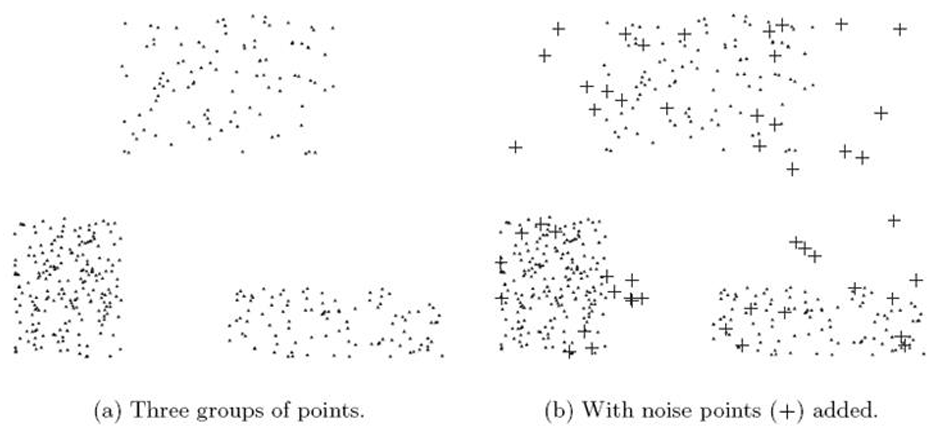
\includegraphics[scale=0.7]{images/noise-example.PNG}
    \caption{An example showcasing the effect of inconsistent or inaccurate data. Noisy data creates indistinguishable bridges between clusters.}
\end{figure}

\noindent
\textbf{Data Preprocessing} addresses the problems of data quality by focusing on the following tasks:

\begin{itemize}
    \item \textbf{Data Cleaning}: Fill in missing values, identify / remove outliers, resolve inconsistencies, etc.
    \item \textbf{Data Integration}: Integration of multiple databases, datasets, or files.
    \item \textbf{Data Reduction}: Dimensionality reduction, numerosity reduction, data compression, etc.
    \item \textbf{Data Transformation and Discretization}: Normalization, etc.
\end{itemize}

\subsection{Data Cleaning}
\textbf{Data Cleaning} is the process of converting the data to a more consistent, accurate and complete state.
\textbf{Noisy data} can be handled in the following ways (and many more):

\begin{itemize}
    \item Sort the data and partition it into equal-sized bins. Smooth the bins by bin-mean, bin-median, bin-boundaries (all elements become either the min. or max. value of the bin), etc.
    \item Clustering to detect and remove outliers.
    \item Train a supervised model on the data. Remove instances that are not correctly predicted by this model.
    \item Use a script to detect suspicious values. Check these values with a domain expert.
\end{itemize}

\noindent
Just because data is missing does not mean that it is useless.
\textbf{Missing values} can be resolved in the following ways (and many more):

\begin{itemize}
    \item Ignore the record (not effective when the percentage of missing values per variable varies considerably).
    \item Fill in the missing values manually (tedious and often infeasible).
    \item Fill the missing values in with a global constant (e.g. \textit{"unknown"}).
    \item Fill the missing values in with the variable mode, median, or mean for nominal, ordinal, and continuous variables respectively.
    \item Fill the missing values in with the most probable values (predicted by a model using the other variables available).
\end{itemize}

\subsection{Data Integration} \label{sec:integration}
\textbf{Data Integration} is the process of combining data from multiple sources into a coherent store.
Possible problems that can arise during integration include different variables having the same name, similar variables having different names, or there being many redundant variables.
For \textit{discrete} variables, redundant variables may be detected through a test of independence, e.g. the \textbf{Chi-Squared Test}.
Assume we need to test two discrete variables for independence: \textit{Tax Reform} and \textit{Income Level}:

\begin{figure}[h!]
    \centering
    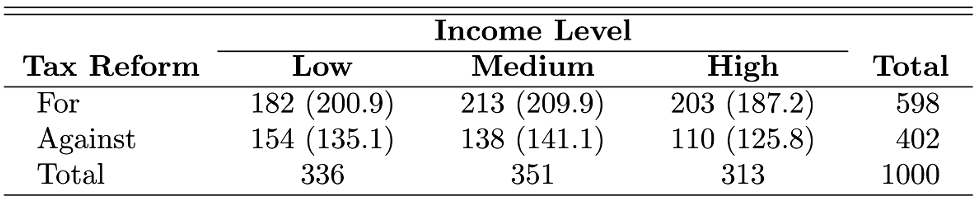
\includegraphics[scale=0.75]{images/chi-squared-example.PNG}
    \caption{The contingency table with the observed and expected frequencies of \textit{Tax Reform} and \textit{Income Level}. The expected frequencies are computed under the assumption that the variables are independent, e.g. $expFreq(Low, For) = \displaystyle\frac{336}{1000} \cdot \frac{598}{1000} \cdot 1000 \approx 200.9$.}
\end{figure}

\newpage
\noindent
We combine the observed and expected frequencies into one \textbf{Chi-Squared} statistic:
\[ \chi^2 = \sum \frac{(obsFreq - expFreq)^2}{expFreq} \]

\noindent
Next we calculate the degrees of freedom of the test:
\[ v = (r - 1) \cdot (c - 1) \]

\noindent
Where $r$ is the number of rows and $c$ is the number of columns in the contingency table.
For our above example we get $\chi^2 \approx 7.85$ and $v = 2$. 
This gives us a $p$-value of $p \approx 0.02$, which, on a significance level of $\alpha = 0.05$, means that the null hypothesis of variable independence is rejected (i.e. the variables are \textit{dependent}).

\noindent
\\
For \textit{continuous} variables, redundant variables may be detected through \textbf{Covariance Analysis}:
\[ Cov(A, B) = \mathbb{E}[(A - \bar{A})(B - \bar{B})] = \frac{\sum_{i = 1}^n (a_i - \bar{A})(b_i - \bar{B})}{n} \]
\[ Cor_{A, B} = \frac{Cov(A, B)}{\sigma_A \sigma_B} \]

\noindent
Where $\bar{A}, \bar{B}$ are the expected values of $A$ and $B$, $\sigma_A, \sigma_B$ are the standard deviations of $A$ and $B$, and $Cor_{A, B}$ is the \textbf{Correlation Coefficient} (always within $[-1, 1]$).
If two variables $A, B$ are independent, then $Cov(A, B) = 0$.
The converse is not always true, as a covariance of 0 only guarantees no \textit{linear} dependence.

\begin{figure}[h]
    \centering
    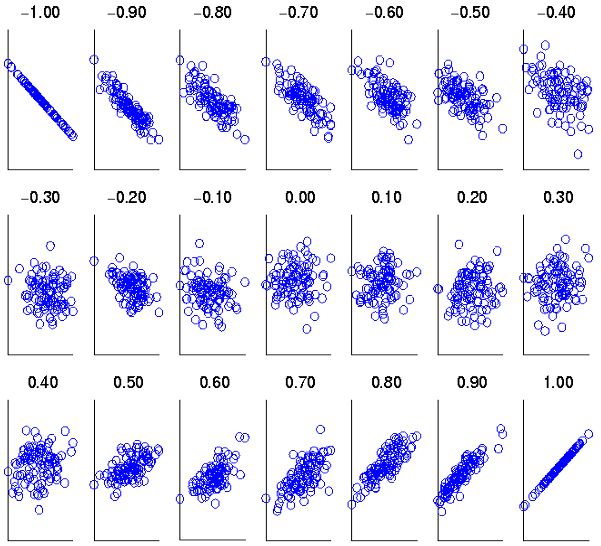
\includegraphics[scale=0.9]{images/covariance.PNG}
    \caption{Scatter plots illustrating correlation from -1 to 1.\label{fig:correlation}}
\end{figure}

\newpage
\subsection{Data Reduction}
\textbf{Data Reduction} is the process of obtaining a reduced representation of the dataset that is smaller in volume, yet produces the same analytical results.
Data reduction can refer to either \textbf{Dimensionality Reduction} (e.g. removing unimportant variables), or \textbf{Numerosity Reduction} (reducing the amount of instances).

\noindent
\\
A common technique for dimensionality reduction is \textbf{Principal Component Analysis (PCA)}.
PCA is a procedure that converts a set of observations of \textit{possibly correlated} variables into a set of values of \textit{uncorrelated} variables called \textbf{Principal Components}.
The first principal component has as high a variance as possible, each succeeding component has the highest variance possible under the constraint that it has to be \textit{orthogonal} (i.e. uncorrelated) to the previous components.
Note that PCA can only be used on numeric variables and is an example of feature \textit{generation}, not \textit{selection}.

\begin{figure}[h]
    \centering
    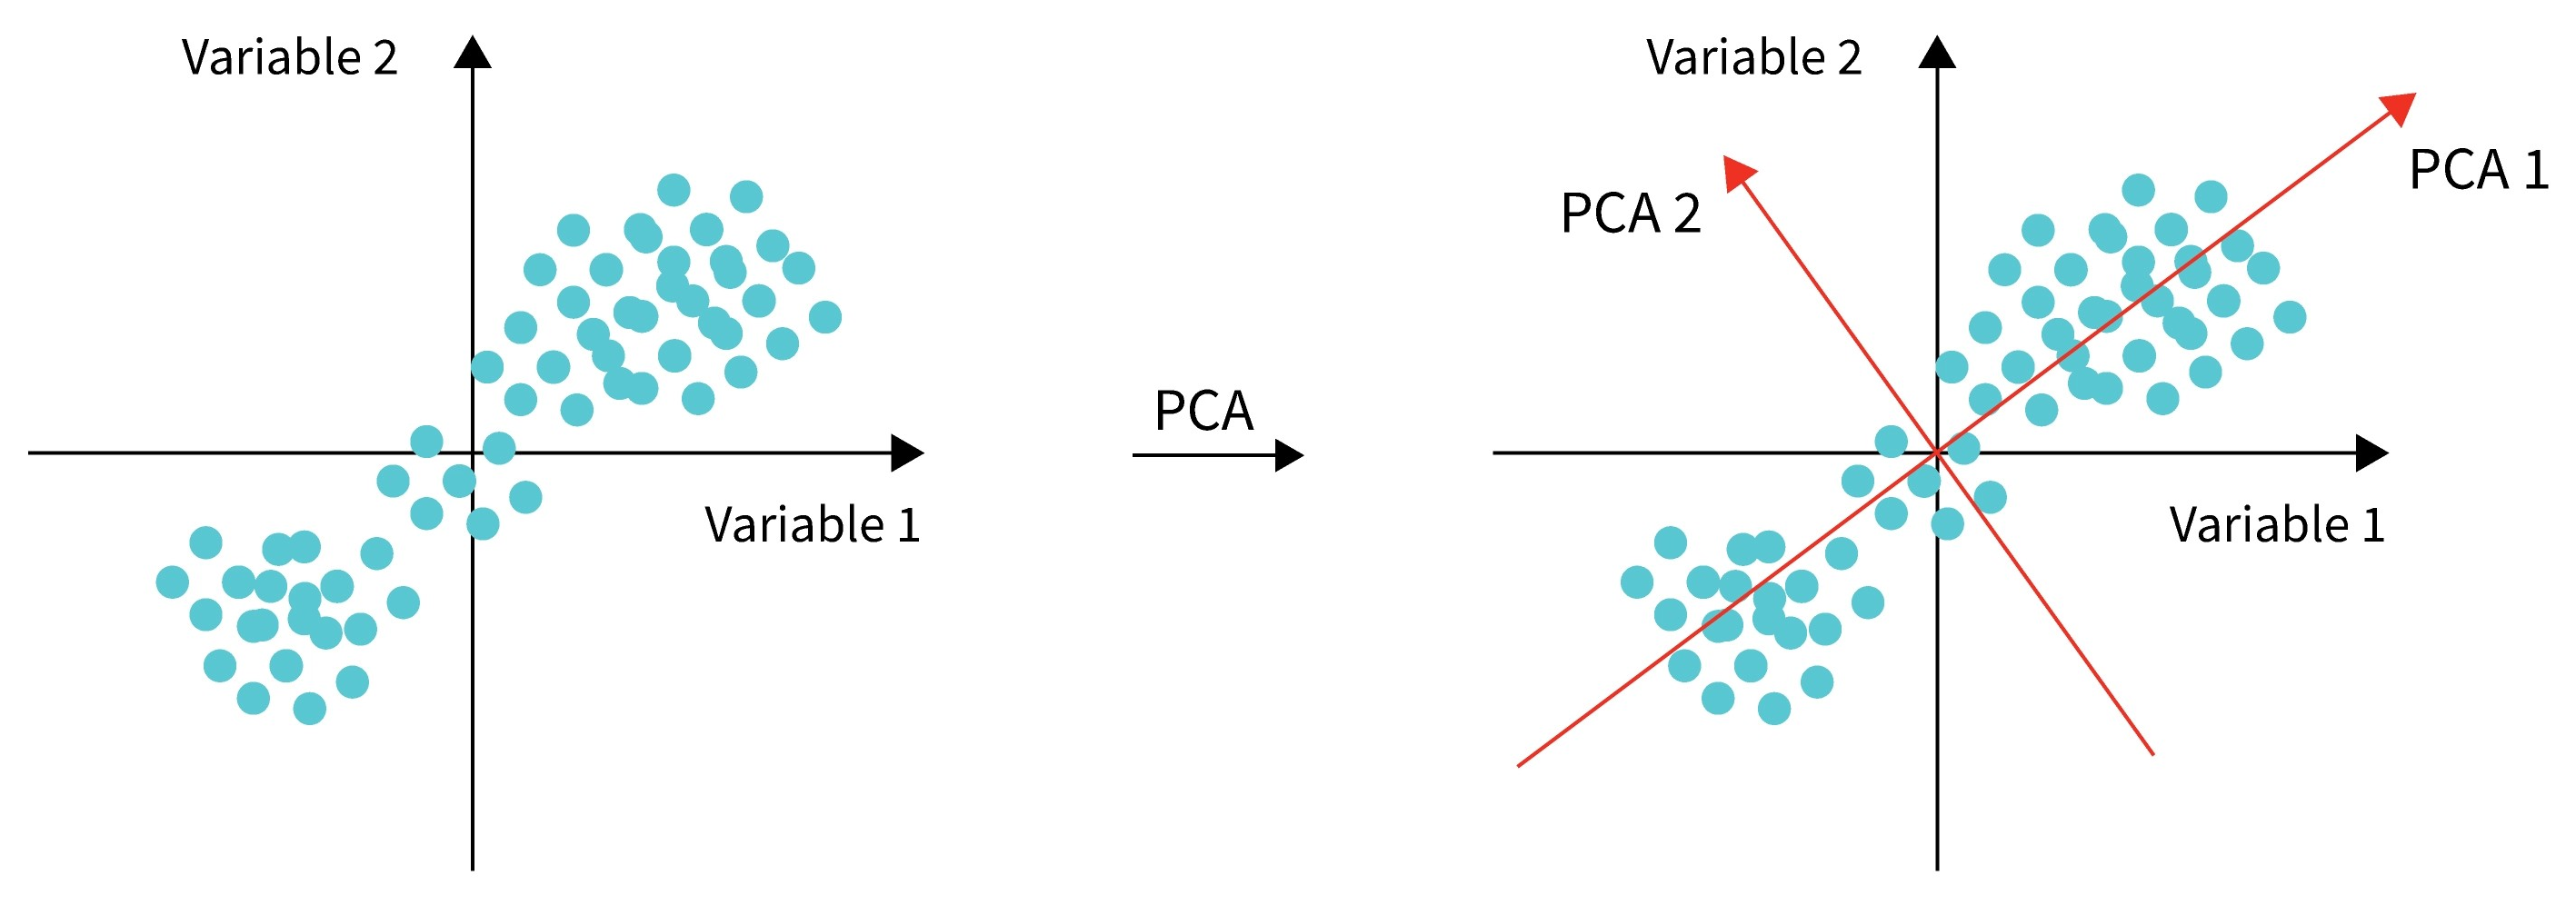
\includegraphics[scale=0.15]{images/pca-example.png}
\end{figure}

\noindent
Assume we have a data matrix $D$ with $n$ rows representing $n$ instances and $p$ columns representing $p$ (numeric) variables.
The PCA algorithm works as follows:

\begin{enumerate}
    \item Standardize $D$ such that each column has a mean of 0.
    \item Compute the covariance matrix of $D$: $S = D^T D$.
    \item Compute the matrix $U$ of $p$ independent eigenvectors $[u_1, u_2, ... , u_p]$ and a diagonal matrix $\Lambda$ with corresponding $n$ eigenvalues $\lambda_1, \lambda_2, ... , \lambda_p$: $S = U \Lambda U^{-1}$.
    \item Compute the new data matrix $D^\prime = DU$. The $i$th variable in this matrix is a linear combination of the original variables through the $i$th eigenvector $u_i$, with a variance of $\lambda_i$. Each pair of new variables has a covariance of 0, and the variables are ordered by how much variance they capture.
\end{enumerate}

\noindent
Another common technique for dimensionality reduction is \textbf{Multidimensional scaling}.
Assume we have the same data matrix $D$ as before.
The goal of multidimensional scaling is to find another set of variables $Z$, such that for any two instances $x_i, x_j$ the distance $d_{ij}^Z$ is very close to $d_{ij}^X$.
The algorithm for multidimensional scaling works as follows:

\begin{enumerate}
    \item Assign instances to arbitrary coordinates in the space based on $Z$.
    \item Create the distance matrix $D^Z$ using the euclidean distance between all pairs of instances.
    \item Compare $D^Z$ to $D^X$ using the \textbf{stress function}: $\sqrt{\sum_{i \neq j} (d_{ij}^Z - d_{ij}^X)^2}$.
    \item Adjust the coordinates of each point in the direction that minimizes the stress function.
    \item Repeat step 2 through to 4 until stress converges.
\end{enumerate}

\newpage
\begin{figure}[h]
    \centering
    \begin{subfigure}{.5\textwidth}
        \centering
        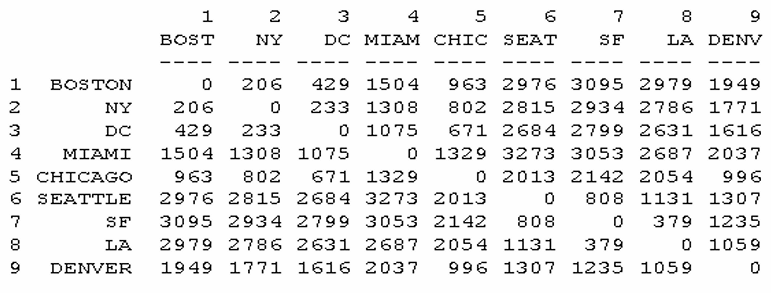
\includegraphics[width=0.9\linewidth]{images/mds-example1.PNG}
    \end{subfigure}%
    \begin{subfigure}{.5\textwidth}
        \centering
        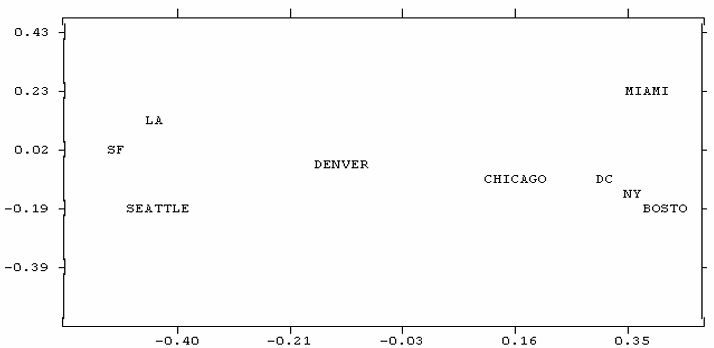
\includegraphics[width=0.9\linewidth]{images/mds-example2.PNG}
    \end{subfigure}
\caption{An example of multidimensional scaling being used to turn a dataset of nine variables into a dataset with only two variables, while keeping the distances the same.}
\end{figure}

\begin{figure}[h]
    \centering
    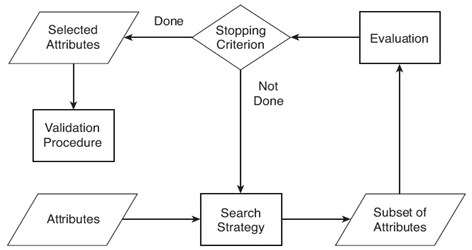
\includegraphics{images/variable-subset-selection.PNG}
    \caption{Another technique for dimensionality reduction is \textbf{Variable Subset Selection}. This process filters out \textit{redundant} variables (e.g. variables whose information is already contained in other variables) and \textit{irrelevant} variables (e.g. a student's ID number is irrelevant for predicting their GPA).}
\end{figure}

\noindent
Numerosity reduction is about reducing data volume by choosing alternative, smaller forms of data representation.
This can be done through \textit{parametric} methods (e.g. assume the data fits some regression model, estimate the model parameters, store only the parameters and discard the data) or \textit{non-parametric} methods:

\begin{itemize}
    \item \textbf{Clustering}: partition the data into a set of clusters, only store the cluster representation (e.g. center, diameter, hierarchical tree structure, etc.).
    \item \textbf{Sampling} is the main technique employed for data selection. Statisticians sample because \textit{obtaining} the entire dataset is too expensive or time consuming. In data mining sampling is used because \textit{processing} the entire dataset is too expensive or time consuming. The key principle of sampling is that a sample will work almost as well as using the entire dataset, as long as the sample is \textit{representative} (it has the same property of interest as the original dataset). Sampling can be done \textit{without replacement}, \textit{with replacement}, or \textit{stratified} (split the data into partitions; draw samples from each).
    \item \textbf{Data Valuation}: assign a numerical value to each instance based on cooperative game theory. A \textit{player} is a single labeled instance, a \textit{coalition} is a subset of labeled instances $S \subseteq D$, and the \textit{value of a coalition} is the performance $v(S)$ of a predictor $h$ trained on $S$ and tested on a validation set $V$. A possible way to assign values to instances is the \textbf{Shapley Value}:
    \[ \varphi_i = \frac{1}{N} \sum_{S \subseteq D \backslash (x_i, y_i)} \binom{N - 1}{|S|}^{-1} \left( v(S \cup \{ (x_i, y_i) \}) - v(S) \right) \]
\end{itemize}

\newpage
\begin{figure}[h]
    \centering
    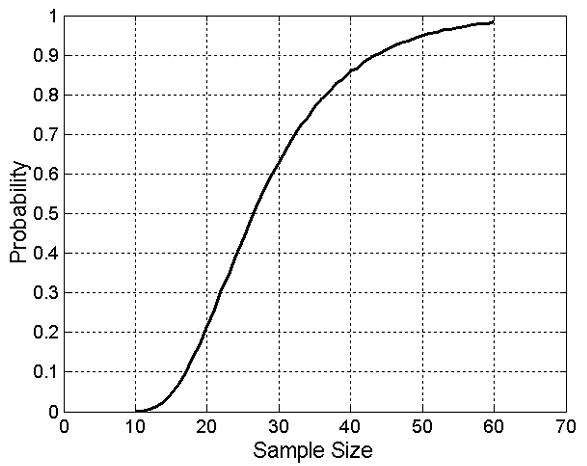
\includegraphics[scale=0.7]{images/sample-size.PNG}
    \caption{Given a dataset of 100 instances, evenly split over 10 classes. What is the probability of sampling at least one instance of every class?}
\end{figure}

\begin{figure}[h]
    \centering
    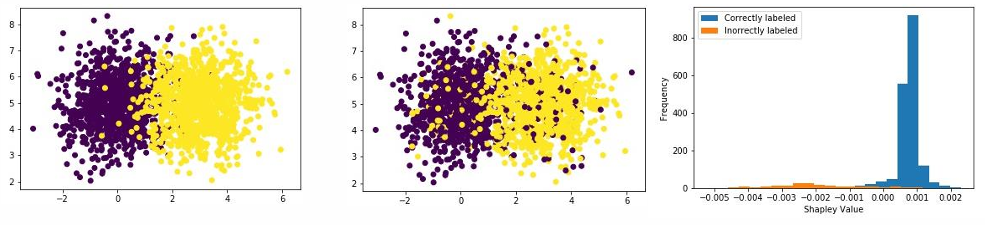
\includegraphics[scale=0.85]{images/shapley.PNG}
    \caption{An example showing how data valuation can be used to identify mislabeled instances. The left figure shows the original two-class problem. The middle figure shows the same problem with randomly flipped labels. The right figure shows a histogram of the shapley values of the instances.}
\end{figure}

\subsection{Data Transformation and Discretization}
\textbf{Normalization} is the process of scaling numeric data to fall within a specified range:

\begin{itemize}
    \item \textbf{Min-Max Normalization} (to $[min_{new}, max_{new}]$):
    \[ v^\prime = \frac{v - min}{max - min} (max_{new} - min_{new}) + min_{new} \]
    \item \textbf{Z-Score Normalization}:
    \[ v^\prime = \frac{v - \mu}{\sigma} \]
\end{itemize}

\newpage
\noindent
\textbf{Discretization} is the process of dividing the range of a continuous variable into intervals.
Common techniques for discretization are \textbf{Binning} and \textbf{Cluster Analysis}; both unsupervised.

\begin{figure}[h]
    \centering
    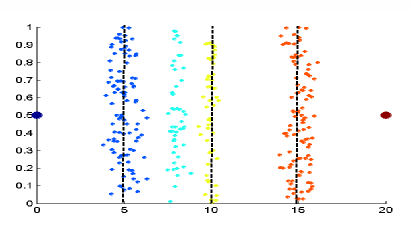
\includegraphics{images/discretization1.PNG}
    \caption{An example of binning with \textit{equal-width} partitioning. The range is divided into $N$ intervals of equal size, with a width of $\frac{max - min}{N}$. This is the most straightforward binning approach, but very susceptible to outliers.}
\end{figure}

\begin{figure}[h]
    \centering
    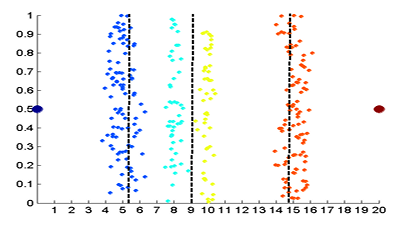
\includegraphics{images/discretization2.PNG}
    \caption{An example of binning with \textit{equal-depth} partitioning. The range is divided into $N$ intervals, each containing roughly the same amount of samples. Managing categorical variables can be tricky.}
\end{figure}

\begin{figure}[h!]
    \centering
    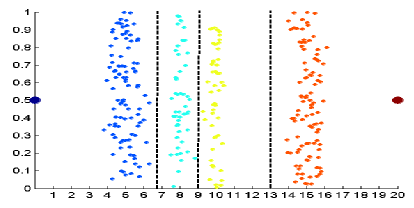
\includegraphics{images/discretization3.PNG}
    \caption{An example of clustering partitioning. The range is divided into $k$ clusters. The example in this figure uses $k$-means clustering. Managing categorical variables can be tricky.}
\end{figure}

%
% Topic 3 - Regression
%
\newpage
\section{Regression}
In a \textbf{Regression Task} we are given (labeled) training data $Tr \subseteq X \times Y$ generated over an unknown probability distribution $Q$ over instance space $X$ and \textit{real-valued} output $Y$.
The goal is to predict a real value $y \in Y$ of a test instance $x$ according to $Q$.

\begin{figure}[h]
    \centering
    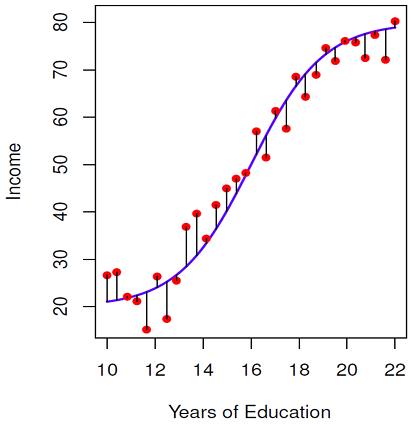
\includegraphics[scale=0.75]{images/population-function.PNG}
    \caption{An example of a regression problem: predicting \textit{Income} from \textit{Years of Education}.}
\end{figure}

\noindent
The difference between prediction and truth is called the \textbf{Residual} or \textbf{Error}.
We assume that there is a relationship between $X$ and $Y$ that can be given by an \textbf{Optimal (Population) Function} $f$: $Y = f(X) + \epsilon$, where $\epsilon$ is an error term that represents the variability in $Y$ that cannot be explained (or reduced) by any model (e.g. measurement error, unmodeled influences, intrinsic variability).
We assume that $\epsilon$ is independent of $X$ with a mean of 0 and a standard deviation of $\sigma_\epsilon$ (\textbf{Homoscedasticity}; If $\epsilon$ is a function of $X$ then there is \textbf{Heteroscedasticity}).
The function $f$ is optimal in the sense that $f(x) = \mathbb{E}[Y | X = x]$.

\noindent
\\
Given a hypothesis space $F$ of functions, the estimation task is to find a function $\hat{f}$ that is close to the optimal function $f$.
We can use this estimated function $\hat{f}$ to do prediction ($\hat{Y} = \hat{f}(X)$) or inference (understand the way $Y$ depends on $X$).
The estimated function $\hat{f}$ can be learned through parametric or non-parametric methods.
With \textit{parametric} methods we assume the form of the optimal function $f$ (e.g. linear, quadratic, etc.):
\[ f(X) = \beta_0 + \beta_1 X_1 + \beta_2 X_2 + ... + \beta_p X_p \]

\noindent
Then we estimate the parameters $\beta$ using the training data $Tr$:
\[ \hat{f}(X) = \hat{\beta}_0 + \hat{\beta}_1 X_1 + \hat{\beta}_2 X_2 + ... + \hat{\beta}_p X_p \]

\noindent
Due to the restricted flexibility of parametric methods, they are very open to \textbf{Underfitting} (it cannot fit the training data closely enough, and because of that fails to predict future observations correctly). Note that not fitting the training data closely enough is not a bad thing on its own, after all it could just be because the data contains a lot of noise. It only becomes a problem when it hinders the predictability of future data.
Parametric methods are often less computationally expensive and require less data than non-parametric models.

\newpage
\noindent
\textit{Non-parametric} methods do not make any assumption about the form of $f$, and therefore are more flexible.
This flexibility means that non-parametric methods are very open to \textbf{Overfitting} (it corresponds to closely to the training data and fails to predict future observations correctly).
Non-parametric methods generally require a lot more data compared to parametric methods.
The less data available, the more susceptible the model becomes to overfitting.

\subsection{Assessing Estimated Functions}
A common way to measure the performance of a model $\hat{f}$ is the \textbf{Mean Squared Error (MSE)}:
\[ MSE = \frac{1}{n} \sum_{i = 1}^n \left( y_i - \hat{f}(x_i) \right)^2 \]

\begin{figure}[h]
    \centering
    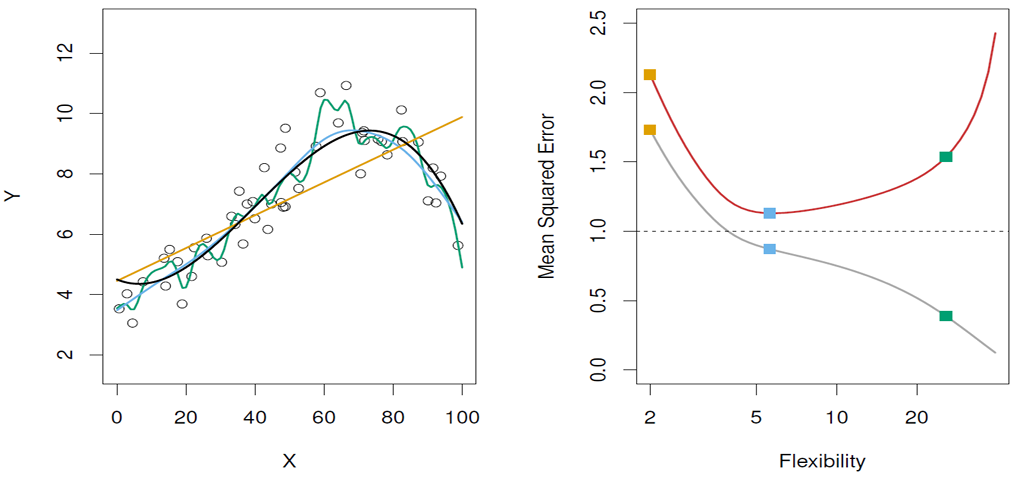
\includegraphics[scale=0.6]{images/mse1.PNG}
    \caption{The left figure shows the optimal function $f$ in black, a linear estimate in orange and two higher order estimates in blue and green. The right figure shows the training MSE in gray, the testing MSE in red and the optimal testing MSE as a dashed line. The yellow estimate is \textit{underfitted}; The green estimate is \textit{overfitted} (training and testing MSE are diverging).\label{fig:mse1}}
\end{figure}

\begin{figure}[h!]
    \centering
    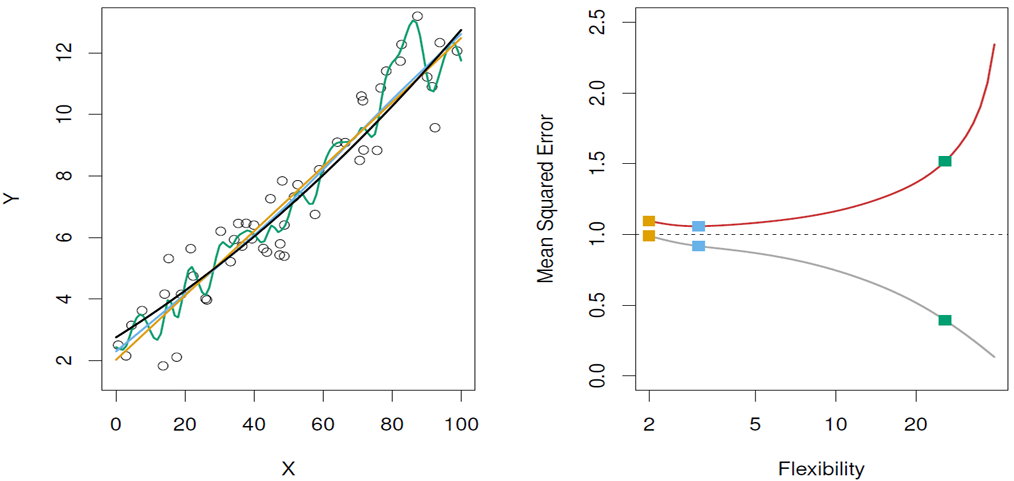
\includegraphics[scale=0.6]{images/mse2.PNG}
    \caption{If the data is almost linear, high flexibility performs worse.\label{fig:mse2}}
\end{figure}

\newpage
\begin{figure}[h]
    \centering
    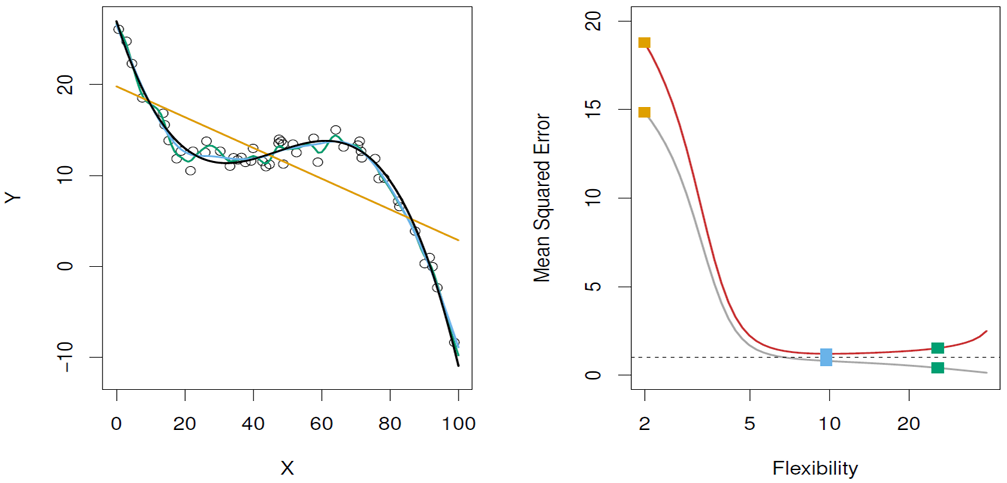
\includegraphics[scale=0.6]{images/mse3.PNG}
    \caption{If the data is very non-linear, low flexibility performs worse.\label{fig:mse3}}
\end{figure}

\noindent
The expected MSE for a given \textit{test} instance $x$ can be decomposed to:
\[ \mathbb{E}\left[ \left( y - \hat{f}(x) \right)^2 \right] = Var(\epsilon) + Var(\hat{f}(x)) + Bias(\hat{f}(x))^2 \]

\noindent
Where $Var(\epsilon)$ is the variance of the random term (\textbf{Irreducible Error}; we cannot influence this), $Var(\hat{f}(x))$ is the variance of the estimate $\hat{f}$ (the variance over the mean prediction) and $Bias(\hat{f}(x))^2$ is the difference between the true mean $f(x)$ and the expected value of the estimate $\mathbb{E}\left[ \hat{f}(x) \right]$.
Typically, as the flexibility of $\hat{f}$ increases, its variance \textit{increases} and its bias \textit{decreases}.
This is called the \textbf{Bias-Variance Tradeoff}.

\begin{figure}[h!]
    \centering
    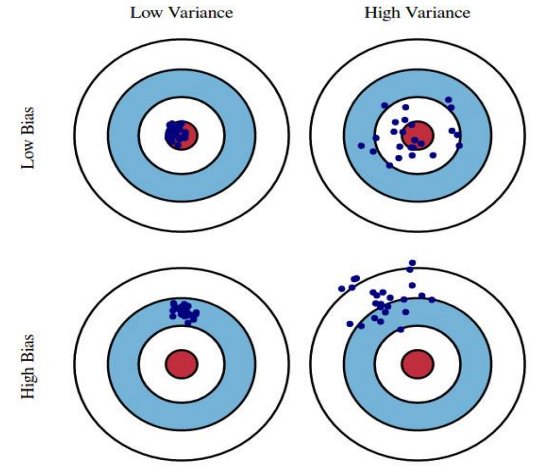
\includegraphics{images/biasvariance.PNG}
    \caption{A graphical illustration of bias and variance.}
\end{figure}

\newpage
\begin{figure}[h!]
    \centering
    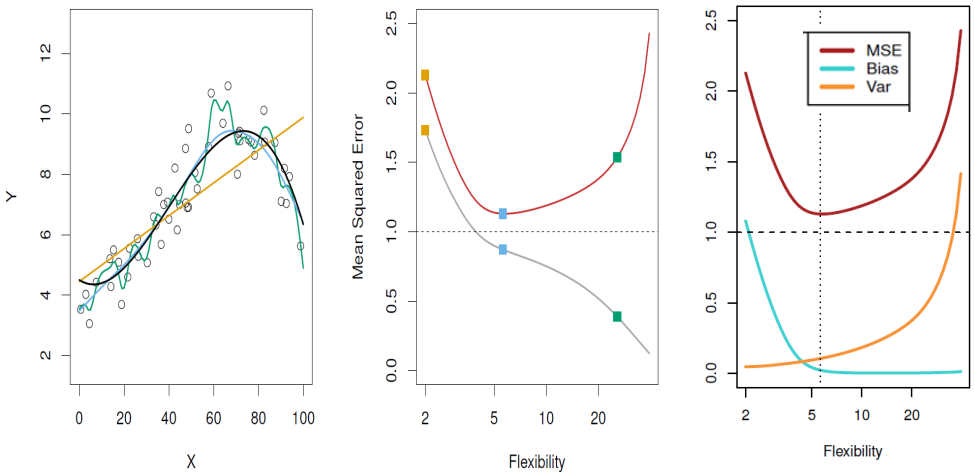
\includegraphics[scale=0.58]{images/biasvariance2.PNG}
    \caption{The right figure shows the MSE of Figure \ref{fig:mse1} decomposed into bias and variance. We want the model to be as close as possible to the intersection between the two.}
\end{figure}

\begin{figure}[h!]
    \centering
    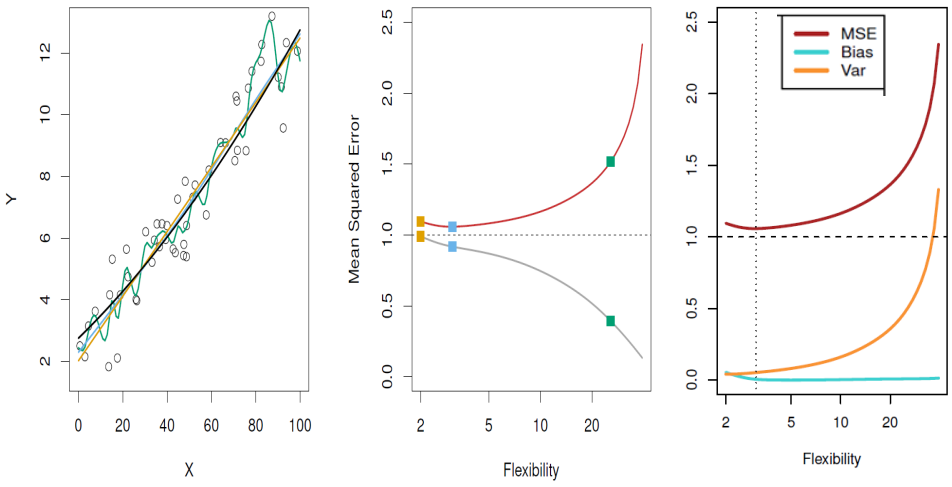
\includegraphics[scale=0.58]{images/biasvariance3.PNG}
    \caption{The right figure shows the MSE of Figure \ref{fig:mse2} decomposed into bias and variance. If the data is almost linear, we quickly suffer from high variance.}
\end{figure}

\begin{figure}[h!]
    \centering
    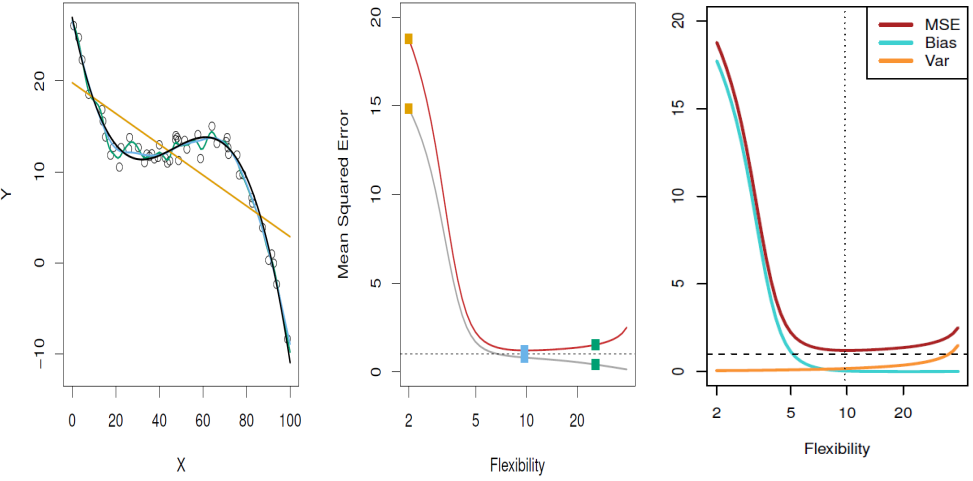
\includegraphics[scale=0.58]{images/biasvariance4.PNG}
    \caption{The right figure shows the MSE of Figure \ref{fig:mse3} decomposed into bias and variance. If the data is very non-linear, we quickly suffer from high bias.}
\end{figure}

\newpage
\subsection{Linear Regression}
\textbf{Linear Regression} is a simple approach to supervised learning. It assumes that $Y$ can be expressed as a linear combination of the input variables.
We \textit{assume} the following true dependence:
\[ Y = \beta_0 + \beta_1 X_1 + \beta_2 X_2 + ... + \beta_p X_p + \epsilon \]

\noindent
Where $\beta_0$ is the intercept, $\beta_i$ is the slope for the $i$th variable $X_i$, and $\epsilon$ is the error term.
If $X_i$ is increased by one unit (and the other variables stay intact), then $\beta_i$ is the average increase in $Y$.
Our estimated function $\hat{f}$ has the following form:
\[ \hat{f}(X) = \hat{\beta}_0 + \hat{\beta}_1 X_1 + \hat{\beta}_2 X_2 + ... + \hat{\beta}_p X_p \]

\noindent
There are various ways to measure the accuracy of linear regression:

\begin{itemize}
    \item \textbf{Residual Sum of Squares (RSS)}: RSS estimates the variance of $Y$ that is left unexplained.
    \[ RSS = \sum_{i = 1}^n \left( y_i - \hat{f}(x_i) \right)^2 \]
    \item \textbf{Residual Standard Error (RSE)}: RSE is the average deviation from the regression line. It is an estimate of the standard deviation of the irreducible error $\epsilon$.
    \[ RSE = \sqrt{\frac{1}{n - 2}RSS} \]
    \item \textbf{Total Sum of Squares (TSS)}: TSS estimates the total variance of $Y$.
    \[ TSS = \sum_{i = 1}^n \left( y_i - \bar{y} \right)^2 \]
    \item \textbf{$R^2$}: $R^2$ estimates the proportion of the variance of $Y$ that is explained. It is also the squared correlation coefficient of $Y$ and $\hat{Y}$.
    \[ R^2 = \frac{TSS - RSS}{TSS} = 1 - \frac{RSS}{TSS} \]
\end{itemize}

\noindent
The additive assumption of linear regression means that the effect of any variable $X_i$ on the output variable $Y$ is independent of the effects of other variables $X_j$.
To avoid this, we can introduce an \textbf{Interaction Term}, but this does introduce non-linearity:
\[ Y = \beta_0 + \beta_1 X_1 + (\beta_2 + \beta_3 X_1)X_2 + ... + \epsilon \]

\noindent
The true function $f(x) = \mathbb{E}[Y | X = x]$ is the function that minimizes $\mathbb{E}[\left(Y - f(x)\right)^2 | X = x]$ (through e.g. gradient descent).
This means that we can estimate the parameters $\beta$ by minimizing the residual sum of squares (RSS).
This leads to the \textbf{Ordinary Least Square Estimator} for linear regression:
\[ \hat{\beta} = \left( X^T X \right)^{-1} X^T Y \]

\noindent
Solving this \textbf{Normal Equation} is efficient for large datasets, but matrix inversion is slow for large numbers of features (and impossible for more features than instances).

\newpage
\noindent
\textbf{Shrinkage Methods} shrink the coefficient-estimates towards zero, reducing the flexibility of the linear regression model and reducing their variance. Two of these shrinkage methods are \textbf{Ridge Regression} and \textbf{Lasso Regression}.

\subsubsection{Ridge Regression}
\noindent
\textbf{Ridge Regression} estimates the parameters $\beta$ by minimizing:
\[ \sum_{i = 1}^n \left( y_i - \hat{\beta}_0 - \sum_{j = 1}^p \hat{\beta}_j X_{ij} \right)^2 + \lambda \sum_{j = 1}^p \left( \hat{\beta}_j \right)^2 = RSS + \lambda \sum_{j = 1}^p \left( \hat{\beta}_j \right)^2 \]

\noindent
Where $\lambda \sum_{j = 1}^p \left( \hat{\beta}_j \right)^2$ is called the \textbf{Regularization Term} or \textbf{L2 Shrinkage Penalty}.

\begin{figure}[h]
    \centering
    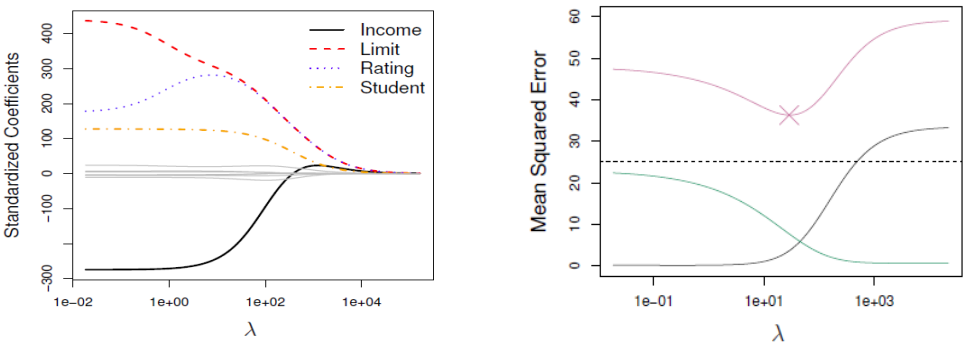
\includegraphics[scale=0.8]{images/regularization.PNG}
    \caption{The effect of the ridge regression regularization parameter $\lambda$ on the size of the coefficients and the MSE. The right figure is decomposed into bias and variance.}
\end{figure}

\noindent
The standard linear regression coefficient estimates are \textit{equivarient}: multiplying $X_i$ by a constant $c$ simply leads to the coefficient estimate $\beta_i$ being scaled by $\frac{1}{c}$ (in other words: regardless of how $X_i$ is scaled, $\beta_i X_i$ will remain the same).
Because of the regularization term, this does \textit{not} hold for ridge regression.
As a result, it is best to apply ridge regression after standardizing the variables.

\noindent
\\
The normal equation for linear regression can also be adapted for ridge regression:
\[ \hat{\beta} = \left( X^T X + \lambda I \right)^{-1} X^T Y \]

\noindent
This has the added benefit of guaranteeing that the equation is invertible.

\subsubsection{Lasso Regression}
\textbf{Lasso Regression} estimates the parameters $\beta$ by minimizing:
\[ \sum_{i = 1}^n \left( y_i - \hat{\beta}_0 - \sum_{j = 1}^p \hat{\beta}_j X_{ij} \right)^2 + \lambda \sum_{j = 1}^p | \hat{\beta}_j | = RSS + \lambda \sum_{j = 1}^p | \hat{\beta}_j | \]

\noindent
Where $\lambda \sum_{j = 1}^p | \hat{\beta}_j |$ is called the \textbf{Regularization Term} or \textbf{L1 Shrinkage Penalty}.

\newpage
\begin{figure}[h]
    \centering
    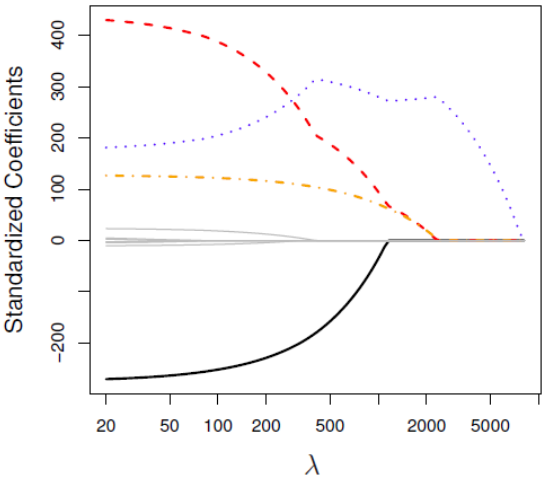
\includegraphics[scale=0.7]{images/lasso-regression.PNG}
    \caption{The effect of the lasso regression regularization parameter $\lambda$ on the size of the coefficients.}
\end{figure}

\noindent
The L1 shrinkage penalty can force some of the $\beta$ estimates to be \textit{exactly} 0 (The L2 shrinkage penalty can only force them \textit{close} to 0).
Hence, lasso regression performs variable selection and can produce \textit{sparse} models (models with only a subset of the variables).

\begin{figure}[h!]
    \centering
    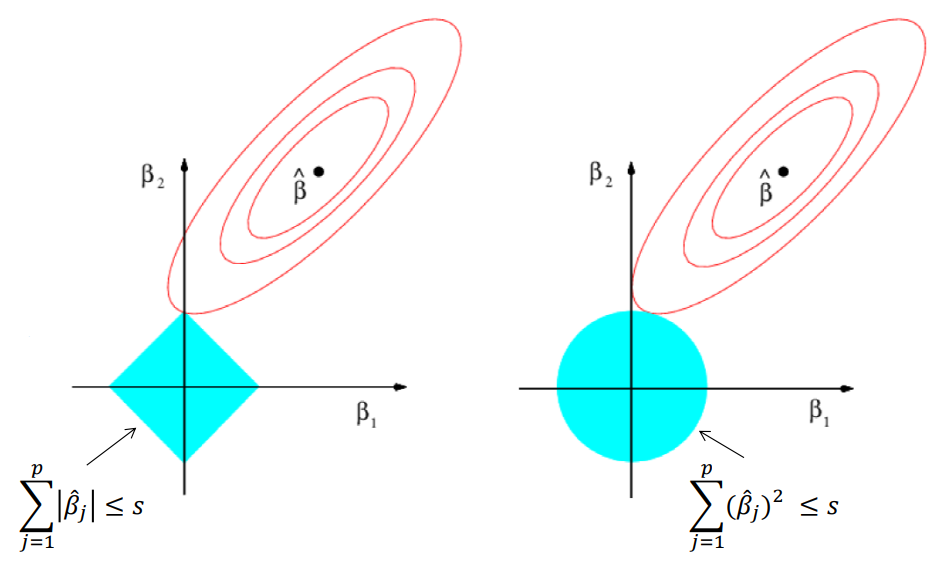
\includegraphics[scale=0.7]{images/lasso-variable-selection.PNG}
    \caption{Lasso and ridge parameter estimation can be seen as minimization problems: minimize the RSS for $\hat{\beta}$, subject to $\sum_{j = 1}^p |\hat{\beta}_j| \leq s$ (lasso) or $\sum_{j = 1}^p (\hat{\beta}_j)^2 \leq s$ (ridge), where $s$ is a regularization parameter similar to $\lambda$. Since the shape of the lasso-constraint is a diamond, the least squares solution might touch the corner of the diamond such that one or more variables will be exactly equal to zero. Since the shape of the ridge-constraint is a circle, this intersection will almost always not lie on one of the axes.}
\end{figure}

\noindent
The lasso loss function is not strictly convex, therefore there may be multiple $\beta$s that minimize this function.
This means that there does not exist a normal equation for lasso regression.

\newpage
\subsection{Nearest-Neighbor}
One of the most popular \textit{non-parametric} regression methods is \textbf{$k$-NN Regression}.
To predict the output value $Y$ for a test instance $X$, it considers a set $NN$ of the $k$ closest instances to $X$ in the training data and takes the average of their output values.
The parameter $k$ controls the flexibility of the $k$-NN regressor (smaller $k$ means a more flexible model).

\begin{figure}[h]
    \centering
    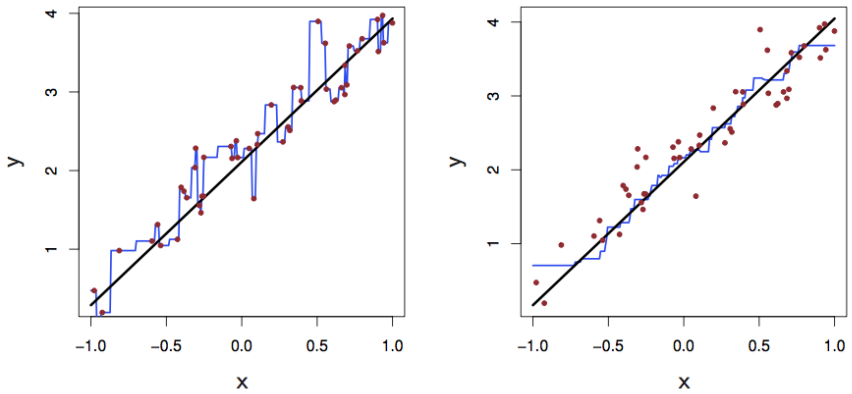
\includegraphics[scale=0.65]{images/knn-regression.PNG}
    \caption{$k$-NN regression in one dimension for $k = 1$ (left) and $k = 9$ (right).}
\end{figure}

\begin{figure}[h!]
    \centering
    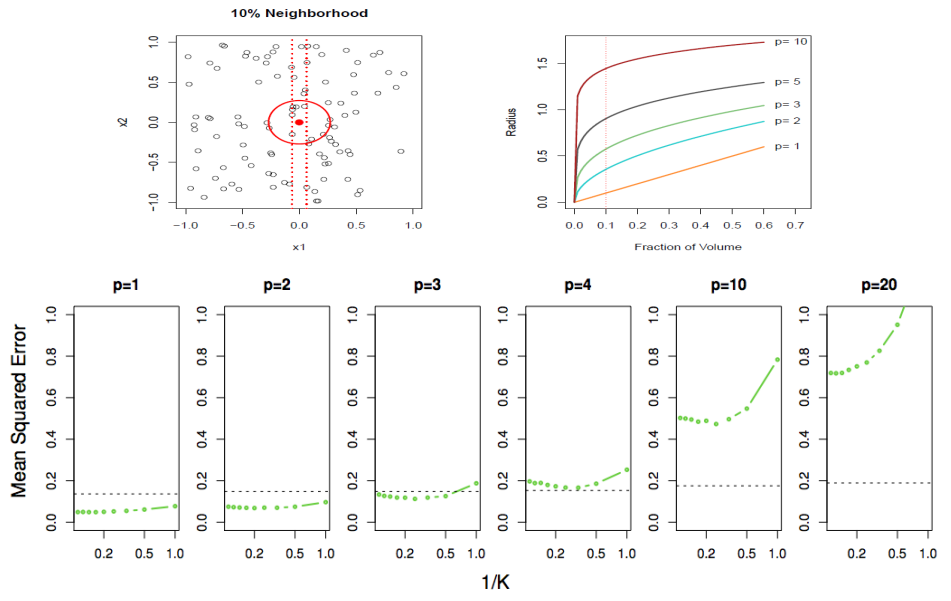
\includegraphics[scale=0.85]{images/knn-dimensions.PNG}
    \caption{$k$-NN regression does not scale well with higher dimensional data. The top two figures show how data becomes sparser when the number of dimensions $p$ increases, leading to a larger radius needed to cover the same fraction of total volume. The bottom figures show how the MSE of $k$-NN regression changes for different values of $k$ and number of dimensions $p$.\label{fig:curse-of-dimensionality}}
\end{figure}

\newpage
\subsection{Regression Trees} \label{sec:regression-trees}
\noindent
Another popular \textit{non-parametric} regression method is \textbf{Regression Trees}.
A regression tree is a tree where each interior node tests an input variable, each branch corresponds to values of the tested input variable and each leaf is labelled by a value $r$.
It is a \textit{piecewise} function of the input variables.

\begin{figure}[h]
    \centering
    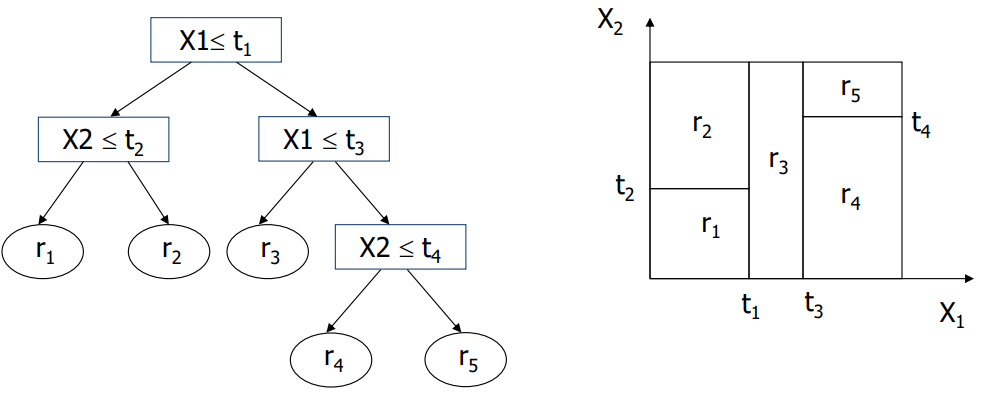
\includegraphics[scale=0.7]{images/regression-tree.PNG}
    \caption{An example of a regression tree.}
\end{figure}

\noindent
A regression tree is learned by minimizing the residual sum of squares (RSS):
\[ RSS = \sum_{j = 1}^J \sum_{i \in R_j} \left( y_i - r_j \right)^2 \]

\noindent
Where $J$ is the number of regions $R_j$ and $r_j$ is the regression value associated with $R_j$.
Globally minimizing the RSS of a regression tree is computationally intractable, so instead we learn regression trees through several steps of determining the optimal variable and threshold to split on:

\begin{enumerate}
    \item Find the next variable $X_j$ to split on with threshold $t_j$ by minimizing:
    \[ RSS(X_j, t_j) = \sum_{i \in R_{j1}} \left( y_i - r_j \right)^2 + \sum_{i \in R_{j2}} \left( y_i - r_j \right)^2 \] Where $R_{j1}$ is all instances $X_i \leq t_j$ and $R_{j2}$ is all instances $X_i > t_j$.
    \item Create two new children for the current node: one for instances $X_i \leq t_j$ and one for $X_i > t_j$.
    \item For each child: if the RSS of the training instances is below a predetermined threshold, then assign the node a regression value equal to the average output value of the training instances. Otherwise, repeat the algorithm from the child node.
\end{enumerate}

\noindent
Regression trees are very sensitive to overfitting (we can always train a tree with an RSS over all regions of 0).
To (partially) overcome this problem, we can apply \textbf{Tree Pruning}.
Trees in general have high variance and low bias.
Tree pruning \textit{reduces} the variance, but \textit{increases} the bias, meaning we need to decide when to start and stop pruning.

\newpage
\begin{figure}[h]
    \centering
    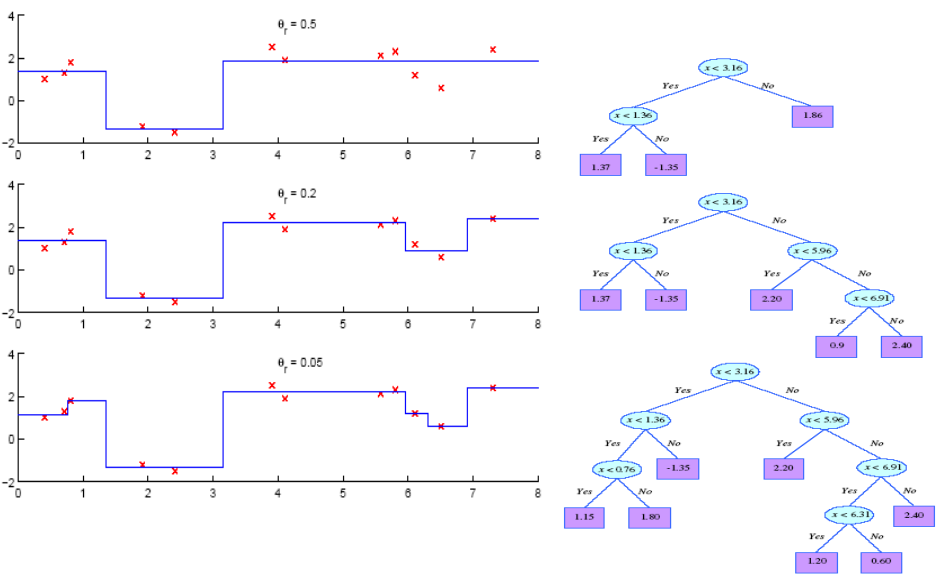
\includegraphics[scale=0.75]{images/regression-tree-pruning.PNG}
    \caption{There are two approaches to avoid overfitting in regression trees. \textbf{(1) Pre-Pruning}: Stop growing the tree earlier, before the point where it perfectly classifies the training data (usually done by tweaking the stopping threshold in the learning algorithm). \textbf{(2) Post-Pruning}: Allow the tree to overfit on the data, then prune after. To decide when to stop pruning a separate validation set is used: when the error on the validation set grows, pruning is stopped.}
\end{figure}

\noindent
A variation of regression trees is \textbf{Model Trees}: a regression tree with a linear regression model in each leaf.
Model trees are trained similarly to regression trees: choosing variables and thresholds for which the RSS of the regression models in the leaves are minimized.
Due to the necessity of training the regression models, model trees are more computationally expensive than regression trees.
However, it is unclear whether model trees are more sensitive to overfitting, since they can often be shorter.

%
% Topic 4 - Classification
%
\newpage
\section{Classification}
In a classification problem we are given a set $\{ X_i \}_{i \in \{ 1, ... , p \}}$ of $p$ input variables that define instance space $X$, a \textit{discrete} variable $Y$, an unknown joint-probability distribution $P(x, y)$ over $X \times Y$, and training data $Tr$ identically and independently sampled from $X \times Y$.
The goal is to find the most probable classification $y \in Y$ of a new instance $x$ according to $P(x, y)$.

\noindent
\\
Each tuple $(x, y) \in X \times Y$ is a value of a random variable $Z$ defined over $X \times Y$ by the probability distribution $P(x, y)$.
If we sample with replacement from $X \times Y$ according to $P(x, y)$, we receive training data $Tr = \{ (x_1, y_1), (x_2, y_2), ... , (x_n, y_n) \}$.
This means that $Tr$ is a realization of $n$ random variables $Z_i$.
We assume that:

\begin{itemize}
    \item The random variables $Z_i$ are \textbf{independent}: $P(Z_i | Z_1, ... , Z_n) = P(Z_i)$. Independent sampling ensures that training instances are selected independently according to the unknown distribution $P(x, y)$, thus we do not need to model the dependency \textit{between} training instances in $Tr$.
    \item The random variables $Z_i$ are \textbf{identically distributed} (i.e. they all have the same distribution $P(x, y)$). Identically distributed sampling ensures that new instances to be classified will be generated by the same distribution $P(x, y)$ (we have a \textit{"bridge"} between the past and future).
\end{itemize}

\noindent
There exist two types of classifiers: \textbf{Discrete Classifiers} (classifiers that directly assign a class label to an instance) and \textbf{Scoring Classifiers} (classifiers that produce a numerical score for each class label that can be assigned to an instance).

\noindent
\\
To solve the classification problem for a new instance $x$ we can assume that we know the \textit{prior probability} $P(y)$, the \textit{likelihood} $P(x | y)$ for each $y \in Y$ and the \textit{evidence} $P(x)$.
We can then compute the \textit{posterior probability} $P(y | x)$ for each $y \in Y$ according to \textbf{Bayes' Rule}:
\[ P(y | x) = \frac{P(x | y)P(y)}{P(x)} \]

\begin{figure}[h!]
    \centering
    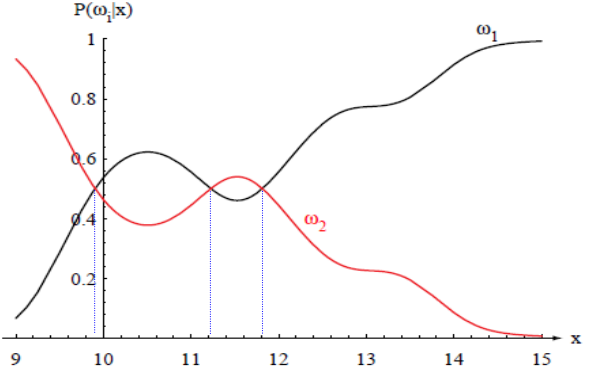
\includegraphics[scale=0.7]{images/bayes-classification.PNG}
    \caption{The winning class is determined using the \textbf{Optimal Bayes Rule}: $y = \displaystyle\argmax_{y \in Y} P(y | x)$. For two-class classification, the probability of misclassifying an instance is given by: $P(\text{error}) = \int_{R_2} P(x | y_1) P(y_1) dx + \int_{R_1} P(x | y_2) P(y_2) dx$, where $R_1$ is the region where class 1 gets chosen and $R_2$ is the region where class 2 gets chosen.}
\end{figure}

\newpage
\subsection{Naive Bayes}
The most popular \textit{parametric} classifier is \textbf{Naive Bayes}.
The Naive Bayes classifier solves the computational problem of the optimal bayes rule by assuming that all variables are conditionally independent (see Appendix \ref{app:math}):
\[ \hat{y} = \argmax_{y \in Y} \prod_{i = 1}^p P(x_i | y) P(y) \]

\noindent
The Naive Bayes classifier does not employ any search in the hypothesis space; it just multiplies probability estimates.
For \textit{discrete} variables we can estimate $P(x_i | y)$ (or $P(X = v | y)$ for a discrete value $v$) using the following methods:

\begin{itemize}
    \item \textbf{Relative Frequency}: $\displaystyle\frac{n_{(X = v | y)}}{n_y}$, where $n_{(X = v | y)}$ is the number of instances that belong to class $y$ and have value $v$ for feature $X$, and $n_y$ is the total number of instances belonging to class $y$.
    \item \textbf{$m$-Estimate of Accuracy}: $\displaystyle\frac{n_{(X = v | y)} + mp}{n_y + m}$, where $p$ is the prior probability of $P(X = v)$ (usually $\frac{1}{|Y|}$), and $m$ is the weight of $p$.
\end{itemize}

\noindent
For \textit{continuous} variables we assume that $P(x_i | y)$ follows some distribution, e.g. Gaussian:
\[ \frac{1}{\sqrt{2\pi}\sigma_i} e^{-\displaystyle\frac{1}{2\sigma_i^2}(x_i - \mu_i)^2} \]

\noindent
Estimating the mean $\mu_i$ and standard deviation $\sigma_i$ is done from the data.
In summary:

\begin{itemize}
    \item Naive Bayes is a \textit{scoring} classifier, however the estimated probabilities can be \textit{too} extreme.
    \item Naive Bayes can be a linear or non-linear method, depending on the properties of the input variables (see Appendix \ref{app:math}).
    \item Naive Bayes does not have any parameter to control the bias-variance trade-off (the only way is explicit feature selection; not part of the model).
\end{itemize}

\subsection{Logistic Regression}
\noindent
Another \textit{parametric} classification method is \textbf{Logistic Regression}.
Logistic regression comes from the idea of using linear regression for classification, which has certain issues (e.g. if $Y$ can only be 0 or 1, what to do with 0.5? 1.5? -1?).
Logistic regression solves these issues by predicting $P(Y = 1 | X)$ using the \textbf{Sigmoid Function} or the \textbf{Softmax Function} (for more than two classes):
\begin{align*}
    P(Y = 1 | X) = \frac{e^{\beta_0 + \beta_1 X_1 + ... + \beta_p X_p}}{1 + e^{\beta_0 + \beta_1 X_1 + ... + \beta_p X_p}} && P(Y = k | X) = \frac{e^{\beta_{0k} + \beta_{1k} X_1 + ... + \beta_{pk} X_p}}{\sum_{i = 1}^{|Y|} e^{\beta_{0k} + \beta_{1k} X_1 + ... + \beta_{pk} X_p}}
\end{align*}

\noindent
Although these functions are non-linear, the log-odds of the probabilities (\textbf{logits}) are linear in $X$:
\[ \log\left( \frac{P(Y = 1 | X)}{1 - P(Y = 1 | X)} \right) = \beta_0 + \beta_1 X_1 + ... + \beta_p X_p \]

\noindent
If we determine the positive class when $P(Y = 1 | X) \geq t$ for some $t \in [0, 1]$, then:
\begin{align*}
   \frac{e^{\beta_0 + \beta_1 X_1 + ... + \beta_p X_p}}{1 + e^{\beta_0 + \beta_1 X_1 + ... + \beta_p X_p}} \geq t && \text{iff} && \beta_0 + \beta_1 X_1 + ... + \beta_p X_p \geq \ln\frac{t}{1 - t}
\end{align*}

\newpage
\noindent
If $t = 0.5$, then $\beta_0 + \beta_1 X_1 + ... + \beta_p X_p = 0$ is the equation of a hyperplane that determines the decision boundary of the logistic regression model.
This means that, even though the logistic function is \textit{non-linear}, logistic regression is a \textit{linear} classifier.

\noindent
We can estimate the parameters $\beta$ of the logistic regression model by maximizing the \textbf{Likelihood Function}:
\[ L(\beta) = \prod_{i = 1}^n P(Y = y_i | x_i) \]

\noindent
Where $P(Y = y_i | x_i)= \displaystyle\frac{e^{\beta_0 + \beta_1 X_1 + ... + \beta_p X_p}}{1 + e^{\beta_0 + \beta_1 X_1 + ... + \beta_p X_p}}$ if $y_i = 1$ or $\displaystyle\frac{1}{1 + e^{\beta_0 + \beta_1 X_1 + ... + \beta_p X_p}}$ if $y_i = 0$.
Since this formula has no closed-form solution, we can solve it numerically using e.g. gradient ascent.
The variance of logistic regression can be reduced using shrinkage methods based on ridge regression (\textbf{Ridge Logistic Regression}).

\subsection{Support Vector Machines}
\noindent
Another \textit{parametric} classification method is \textbf{Support Vector Machines (SVM)}.
SVMs approach the two-class problem in a direct way: trying to separate the classes directly in instance space $X$.
If this impossible, SVMs either soften what we mean with \textit{"separate"} or enlarge the instance space $X$ so that separation \textit{is} possible.
SVMs work by creating \textbf{Hyperplanes}:
\[ \beta_0 + \beta_1 X_1 + \beta_2 X_2 + ... + \beta_p X_p = 0 \]

\noindent
If $\beta_0 = 0$ the hyperplane goes through the origin, otherwise not.
The vector $\beta = (\beta_1, \beta_2, ... , \beta_p)$ is the \textit{normal vector} of the hyperplane.
If this is a unit vector, then the distance of any point $x = (x_1, x_2, ... x_p)$ to the hyperplane is equal to:
\[ f(X) = \beta_0 + \beta_1 X_1 + \beta_2 X_2 + ... + \beta_p X_p \]

\noindent
Observe that, for the above function $f(X)$, $f(X) > 0$ for all instances on one side of the hyperplane, and $f(X) < 0$ for all instances on the other side of the hyperplane.
$f(X) = 0$ defines a \textit{separating hyperplane}.
Among all possible separating hyperplanes, the goal of an SVM is to find the one that \textit{maximizes} the margin between the two classes (the \textbf{Maximal Margin Classifier}):

\begin{figure}[h!]
    \centering
    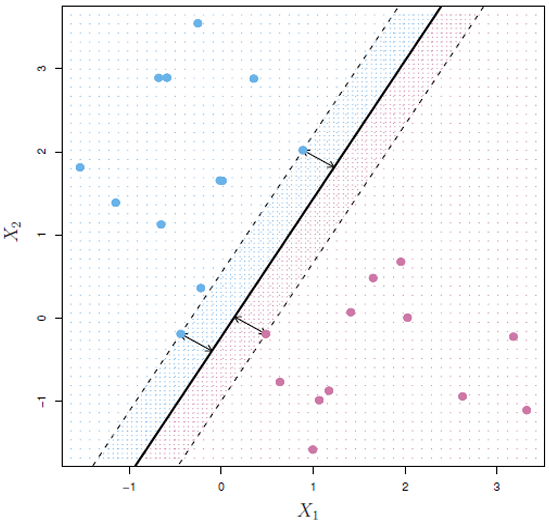
\includegraphics[scale=0.6]{images/svms.PNG}
    \caption{An example of the maximal margin classifier between two linearly-separable classes.}
\end{figure}

\newpage
\noindent
Finding the maximal margin classifier is a constraint optimization problem:
\begin{align*}
    \max_{\beta_0, \beta_1, ... , \beta_p} \quad & M \\
    \text{s.t.} \quad & \sum_{j = 1}^p \left( \hat{\beta}_j \right)^2 = 1 \\
     & y_i \left( \beta_0 + \beta_1 x_{i1} + ... + \beta_p x_{ip} \right) \geq M \\
    \forall \quad & i = 1, ... , N
\end{align*}

\noindent
Where $y_i \in \{-1, 1\}$.
This problem is a \textit{convex} quadratic problem and can thus be solved efficiently.
Unfortunately, most of the time the data is not immediately separable by a linear boundary.

\begin{figure}[h]
    \centering
    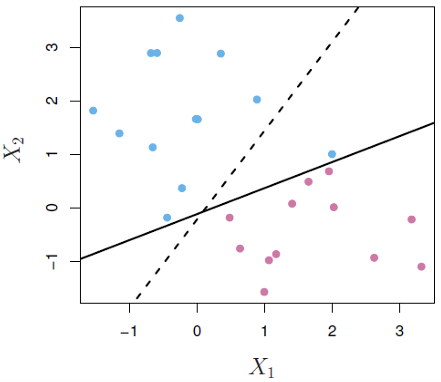
\includegraphics[scale=0.75]{images/svm-noise.PNG}
    \caption{Sometimes data \textit{is} linearly separable, but noise leads to a poor maximum margin classifier.}
\end{figure}

\noindent
One way to solve this problem is maximizing a \textbf{Soft Margin}:
\begin{align*}
    \max_{\beta_0, \beta_1, ... , \beta_p} \quad & M \\
    \text{s.t.} \quad & \sum_{j = 1}^p \left( \hat{\beta}_j \right)^2 = 1 \\
     & y_i \left( \beta_0 + \beta_1 x_{i1} + ... + \beta_p x_{ip} \right) \geq M \left( 1 - \zeta_i \right) \\
     & \sum_{i = 1}^N \zeta_i \leq C, \quad \zeta_i \geq 0 \\
    \forall \quad & i = 1, ... , N
\end{align*}

\noindent
Here $C$ is a regularization parameter: higher $C$ values imply low flexibility \textit{(high bias, low variance)}, lower $C$ values imply high flexibility \textit{(low bias, high variance)}.

\noindent
\\
Sometimes a linear boundary can fail even with a soft margin (e.g. non-linear data).
In this case we can use \textbf{Feature Expansion}: enlarging the space of features by including transformations (e.g. $X^2$, $X^3$, $X_1 X_2$, etc.), going from a $p$-dimensional space to a $P > p$ dimensional space.
Fitting a support-vector classifier in this enlarged space results in a non-linear decision boundary in the original space.

\newpage
\begin{figure}[h]
    \centering
    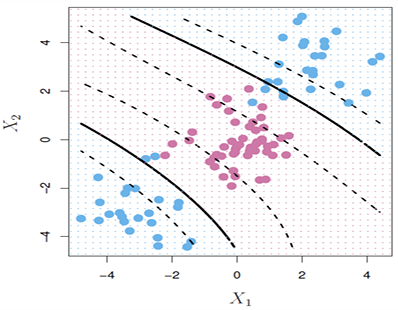
\includegraphics[scale=0.9]{images/svm-nonlinear.PNG}
    \caption{An example of non-linear data that can only be separated through feature expansion.}
\end{figure}

\noindent
Assume that we have function $K$ that computes a similarity for any two instances, an SVM can then be represented as:
\[ f(x) = \beta_0 + \sum_{i = 1}^N \alpha_i K(x, x_i) \]

\noindent
Where $\beta_0$ and $\alpha_i$ can be learned by an SVM.
This function $K$ is called a \textbf{Kernel}, and also allows an SVM to take on a non-linear decision boundary:

\begin{figure}[h]
    \centering
    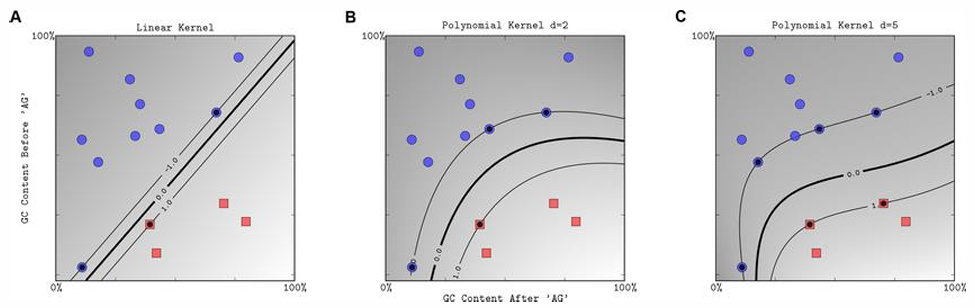
\includegraphics[scale=0.8]{images/svm-kernel.PNG}
    \caption{Maximum margin classifier for a \textit{linear} ($K(x_i, x_j) = x_i^T x_j$) and \textit{polynomial} ($K(x_i, x_j) = \left( \gamma x_i^T x_j + c \right)^d$) kernel.}
\end{figure}

\noindent
A support vector machine is a \textit{discrete} classifier (i.e. it outputs the predicted class $sgn(f(x))$).
To convert a support vector machine to a \textit{scoring} classifier we can either just use the signed distance to the hyperplane $f(x)$, or we can use \textbf{Platt Scaling}:
\[ \frac{1}{1 + e^{A f(x) + B}} \]

\noindent
Where $A$ and $B$ are two scalars that can be learned with maximum likelihood from the data.

\newpage
\subsection{Decision Trees} \label{sec:decision-trees}
A common method for \textit{non-parametric} classification is \textbf{Decision Trees}.
These are identical to \textit{Regression Trees} (Section \ref{sec:regression-trees}), with the only difference being that decision trees hold \textit{classes} in their leaf nodes.
Decision trees are robust against labelling errors and/or missing values in the training data.

\begin{figure}[h]
    \centering
    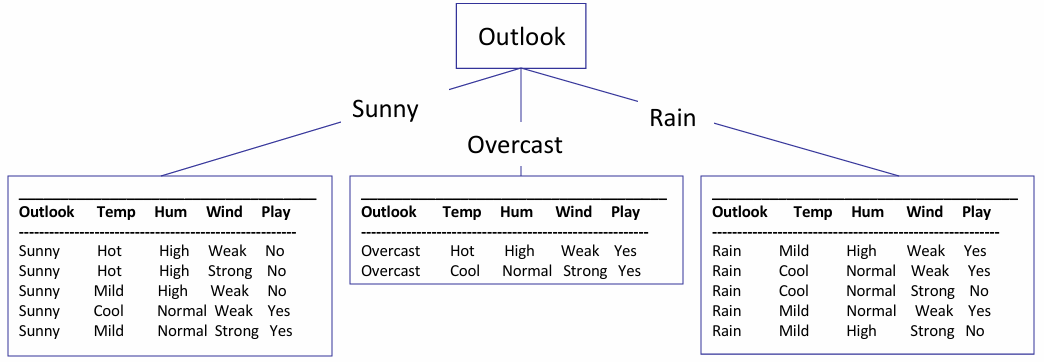
\includegraphics[scale=0.75]{images/decision-tree-learning.PNG}
    \caption{The general procedure for learning a \textit{discrete} decision tree: \textbf{(1)} Choose the best decision variable $X^\prime$ for a node $N$. \textbf{(2)} For each value of $X^\prime$, create a new child node of $N$. \textbf{(3)} Repeat until all the training data is perfectly classified.\label{fig:decision-tree-example}}
\end{figure}

\noindent
Let $S$ be a sample of the training data, with $p^+$ being the proportion of positive examples in $S$ and $p^-$ being the proportion of negative examples in $S$.
We can use \textbf{Entropy} to measure the \textit{impurity} of $S$:
\begin{align*}
    E(S) = -p^+ \log_2 p^+ - p^- \log_2 p^- && \left( E(S) = - \sum_i p_i \log_2 p_i \right)
\end{align*}

\noindent
\textbf{Information Gain} is the expected reduction in entropy caused by partitioning the instances from $S$ according to a decision variables $X^\prime$:
\[ Gain(S, X^\prime) = E(S) - \sum_{v \in \text{domain of } X^\prime} \frac{|S_v|}{|S|} E(S_v) \]

\noindent
Where $S_v$ is the subset of $S$ with value $v$ for $X^\prime$.
Going back to Figure \ref{fig:decision-tree-example},
we can decide which variable should be split on in the $S_{\text{Sunny}}$ branch by computing the information gain for each option:
\begin{align*}
    Gain(S_{\text{Sunny}}, \text{Humidity}) = 0.970, && Gain(S_{\text{Sunny}}, \text{Temperature}) = 0.570, && Gain(S_{\text{Sunny}}, \text{Wind}) = 0.019
\end{align*}

\noindent
Decision tree learning performs a simple-to-complex hill climbing search through the hypothesis space with information gain as the evaluation function.
There is no backtracking and only a single tree is maintained at once, but all training instances are being used.
Decision trees in general have high variance, with larger (deeper) trees having higher variance and lower bias.

\noindent
\\
Decision trees can also be used with \textit{continuous} variables (e.g. temperature as a number instead of a discrete value).
This can be done by either discretizing \textit{before} training, or \textit{during} the training by splitting on the variables similarly to Regression Trees (but instead \textit{maximizing} the information gain).
Since we can set the splitting point anywhere we want, decision trees are \textit{non-linear} classifiers.

\newpage
\begin{figure}[h]
    \centering
    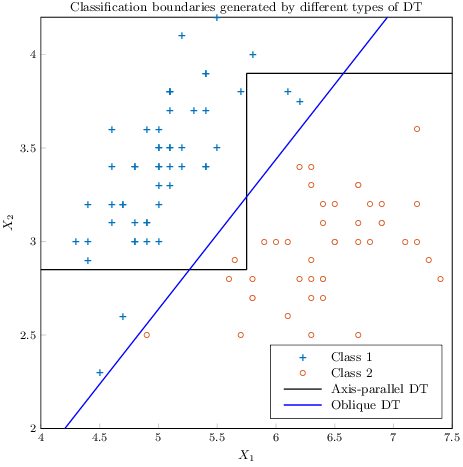
\includegraphics[scale=0.4]{images/oblique-decision-tree.png}
    \caption{\textbf{Oblique Decision Trees} test conditions involving multiple variables. While this does lead to a more expressive representation, finding the optimal split is computationally expensive.}
\end{figure}

\noindent
Decision trees are very prone to overfitting.
We can detect this by observing if only a small number of instances are associated with leaf nodes.
Similarly to Regression Trees, we can avoid overfitting through either \textit{Pre-Pruning} (difficult to do in decision trees, but a common way is to stop expending a leaf node if it gets less than $m$ training instances) or \textit{Post-Pruning}.

\noindent
\\
To apply post-pruning, we need to split the data \textit{randomly} into a \textbf{Growing Set} and a \textbf{Validation Set}.
We can then prune using an algorithm such as \textbf{Reduced-Error Pruning}:

\begin{enumerate}
    \item For each node $d$, evaluate the impact on the validation accuracy of \textit{pruning} $d$ (and all its children).
    \item \textit{Prune} the node $d^\prime$ that improves the validation accuracy the most.
    \item Repeat until further pruning becomes harmful.
\end{enumerate}

\noindent
\textit{Pruning} can either mean completely cutting $d^\prime$ and replacing it with a leaf holding the most common class of the associated training instances (\textbf{Sub-Tree Replacement}), or removing the parent of $d^\prime$ and replacing it with $d^\prime$ (\textbf{Sub-Tree Raising}).

\begin{figure}[h!]
    \centering
    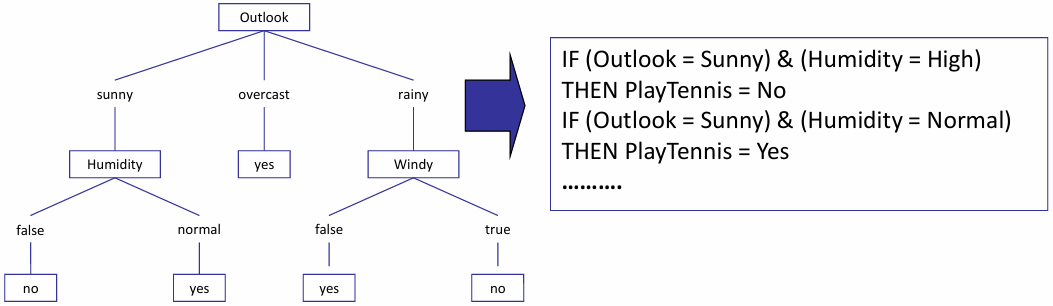
\includegraphics[scale=0.7]{images/rule-post-pruning.PNG}
    \caption{Another form of post-pruning is \textbf{Rule Post-Pruning}: \textbf{(1)} Convert the tree into an equivalent set of rules. \textbf{(2)} Prune each rule independently of others. \textbf{(3)} Sort the rules by their estimated accuracy, and consider them in this order.}
\end{figure}

\newpage
\noindent
Let $S$ be a sample of the training data, with $p_i$ being the proportion of instances of class $i$ in $S$.
To learn a decision tree we need to define an \textbf{Impurity Measure} $I(S)$ that satisfies:

\begin{itemize}
    \item $I(S)$ is minimum iff $p_i = 1$ and $p_j = 0$ for $i \neq j$ (all instances are of the same class).
    \item $I(S)$ is maximum iff $p_i = \frac{1}{I}$ (there is exactly the same amount of instances for all classes).
    \item $I(S)$ is symmetric with respect to $p_1, ... , p_i$.
\end{itemize}

\noindent
The optimal split is the split that maximizes the expected reduction of impurity:
\[ \Delta I(S, V) = I(S) - \sum_a \frac{|S_a|}{|S|} I(S_a) \]

\noindent
Here $\Delta I$ is called a \textbf{Score Measure} or \textbf{Splitting Criterion}.
Aside from entropy, another popular impurity measure is \textbf{Gini Impurity} (measuring how often a randomly chosen element from the set would be miscategorized if it were labeled according to the distribution of $S$):
\[ Gini(S) = 1 - \sum_i \left( p_i \right)^2 \]

\noindent
A big problem for decision trees is variables with many possible values.
These variables fragment data quickly, and as a result often have a high reduction of impurity (the score measure is biased to pick them).
We can solve this by either considering only binary splits, or changing the splitting criterion to penalize variables with many values, for example by using \textbf{Gain Ratio} as splitting criterion:
\[ GainRatio(S, X^\prime) = \frac{Gain(S, X^\prime)}{SplitInfo(S, X^\prime)} = \frac{\Delta I(S, X^\prime)}{- \displaystyle\sum_{v \in \text{domain of } X^\prime} \frac{|S_v|}{|S|} \log_2 \frac{|S_v|}{|S|}} \]

\noindent
The downside of using gain ratio is that it favours unbalanced tests.
Another problem for decision trees is how to deal with missing values during the training.
If a node tests a variable $X_i$ that is missing for some instances, then estimate a probability for each value of $X_i$ for each instance (based on the observed frequencies of $X_i$). These probabilities can be used directly in the information gain formula, so no sampling is required.

\noindent
\\
Another common problem for decision trees is that all the data needs to fit into memory at once.
If this is not possible, a possible solution is to use \textbf{Windowing}:

\begin{enumerate}
    \item Randomly select $n$ instances from the training data and put them in a \textbf{Window Set} $W$.
    \item Train a decision tree on $W$.
    \item Test the tree on the full dataset, keeping track of all the instances that are not classified correctly: $M$.
    \item If the tree performs adequate on the full dataset, keep it. Otherwise add $M$ to $W$ and repeat.
\end{enumerate}

\newpage
\subsubsection{Decision Rules}
\begin{figure}[h]
    \centering
    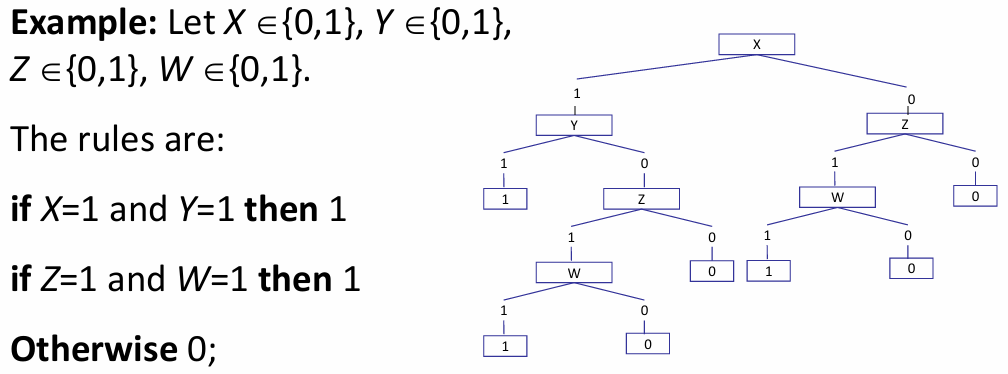
\includegraphics[scale=0.75]{images/decision-rules-vs-trees.PNG}
    \caption{A variation of decision trees is \textbf{Decision Rules}. These are rules of the form $if \left\langle condition \right\rangle then \left\langle class \right\rangle$, and are often more compact and understandable than a decision tree.}
\end{figure}

\begin{figure}[h]
    \centering
    \begin{subfigure}{.5\textwidth}
        \centering
        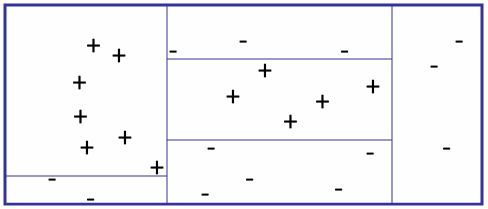
\includegraphics[width=.8\linewidth]{images/decision-tree-bound.PNG}
        \caption{The decision boundary of a decision tree.}
    \end{subfigure}%
    \begin{subfigure}{.5\textwidth}
        \centering
        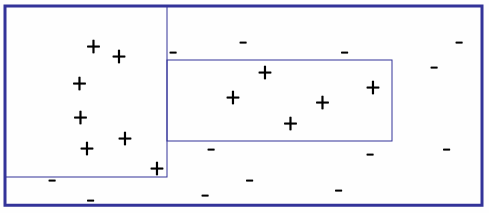
\includegraphics[width=.8\linewidth]{images/decision-rules-bound.PNG}
        \caption{The decision boundary of decision rules.}
    \end{subfigure}
\caption{The difference in decision boundaries between decision trees and decision rules.}
\end{figure}

\noindent
Decision rules can be learned by either converting a tree to rules, or by using specific rule-learning methods, for example \textbf{Sequential Covering} algorithms:

\begin{enumerate}
    \item Given attributes $X$ and examples $Tr$, learn a rule $R$.
    \item Remove all examples covered by $R$ from $Tr$.
    \item Repeat until performance is adequate, then sort the rules by some criterion.
\end{enumerate}

\noindent
Learning a single rule can be done \textbf{Top-Down} (start with a maximally general, add literals one by one; generate-then-test / CN-2) or \textbf{Bottom-Up} (start with maximally specific rule, remove literals one by one; example-driven / AQ Family).
Possible evaluation functions for identifying good rules include \textbf{Relative Frequency} ($\frac{n_c}{n}$ where $n_c$ is the number of correctly classified instances and $n$ is the total number of instances covered by the rule), \textbf{$m$-Estimate of Accuracy} ($\frac{n_c + mp}{n + m}$ where $p$ is the prior probability of the class predicted by the rule and $m$ is the weight of $p$), and Entropy.

\noindent
\\
Rules can be ordered by the order in which they were learned, in order of accuracy, or unordered with a conflict strategy (e.g. an instance covered by conflicting rules gets the classification of the rule that classifies more training instances; if an instance is not covered by any rule, then it gets the classification of the majority class in the training data).

\newpage
\noindent
Similarly to decision trees, decision rules also suffer from high variance.
Smaller sets of shorter decision rules have \textit{low} flexibility (high bias, low variance), while larger sets of longer decision rules have \textit{high} flexibility (low bias, high variance).

\noindent
\\
Just like decision trees, decision rules can be pruned using \textit{pre-pruning} or \textit{post-pruning}, the latter of which includes \textbf{Incremental Reduced Error Pruning}:

\begin{enumerate}
    \item Split the training data $Tr$ into a \textit{growing set} and \textit{pruning set}.
    \item Learn a rule $R$ using the growing set, and prune it using the pruning set.
    \item If the performance of $R$ on the training set is above some threshold, add $R$ to the set of learned rules and remove the instances covered by $R$ from $Tr$.
    \item Repeat from (1) until the above condition fails.
\end{enumerate}

\begin{figure}[h]
    \centering
    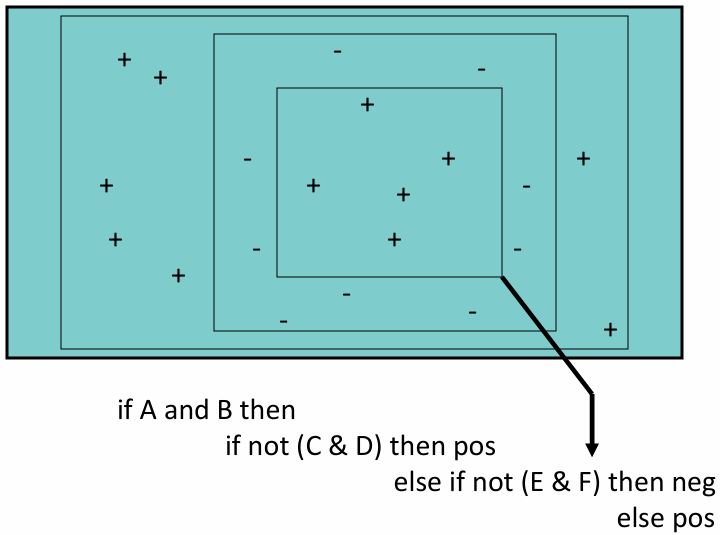
\includegraphics[scale=0.6]{images/decision-rules.PNG}
    \caption{Learning decision rules with exceptions.}
\end{figure}

\noindent
In summary, decision rules are discrete classifiers that can estimate class probabilities by normalizing class scores in each rule.
They are non-linear classifiers, and usually simpler than decision trees on the same data.

\subsection{Nearest-Neighbor}
\noindent
Another common method for \textit{non-parametric} classification is \textbf{Nearest-Neighbor Classification}.
Given an unknown instance $x$, a $k$-NN classifier finds the set $NN$ of the $k$ closest instances to $x$ in the training data:

\begin{itemize}
    \item \textbf{Discrete Classification}: output the majority class among $NN$.
    \item \textbf{Scoring Classification}: estimate class probabilities from $NN$.
\end{itemize}

\noindent
The value of $k$ controls the flexibility of the $k$-NN classifier, with smaller values being more flexible (high variance, low bias).

\newpage
\begin{figure}[h]
    \centering
    \begin{subfigure}{.33\textwidth}
        \centering
        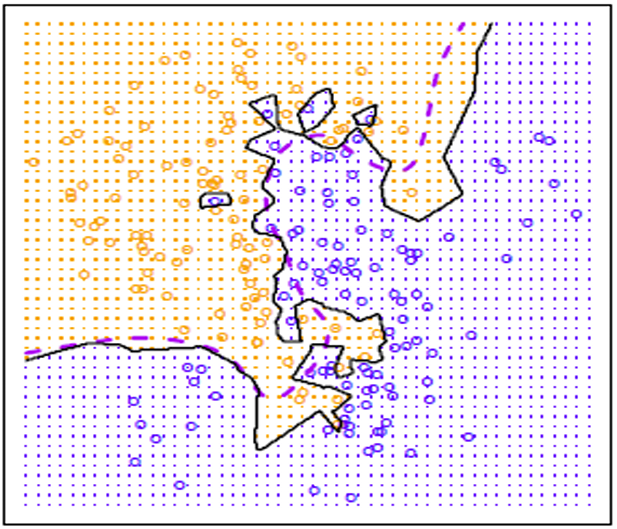
\includegraphics[width=.8\linewidth]{images/knn1.PNG}
        \caption{$k = 1$}
    \end{subfigure}%
    \begin{subfigure}{.33\textwidth}
        \centering
        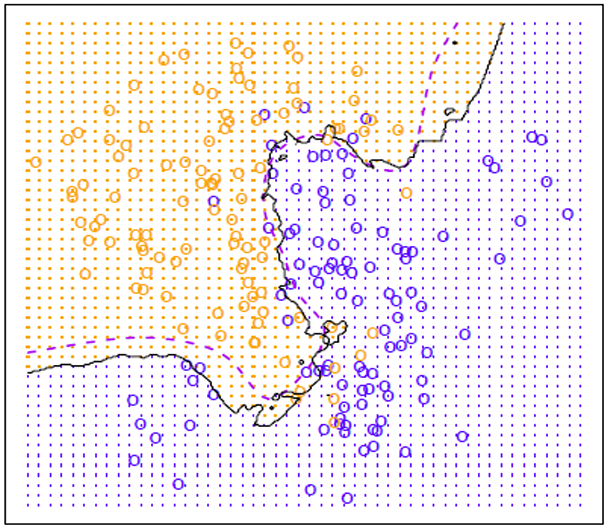
\includegraphics[width=.785\linewidth]{images/knn10.PNG}
        \caption{$k = 10$}
    \end{subfigure}%
    \begin{subfigure}{.33\textwidth}
        \centering
        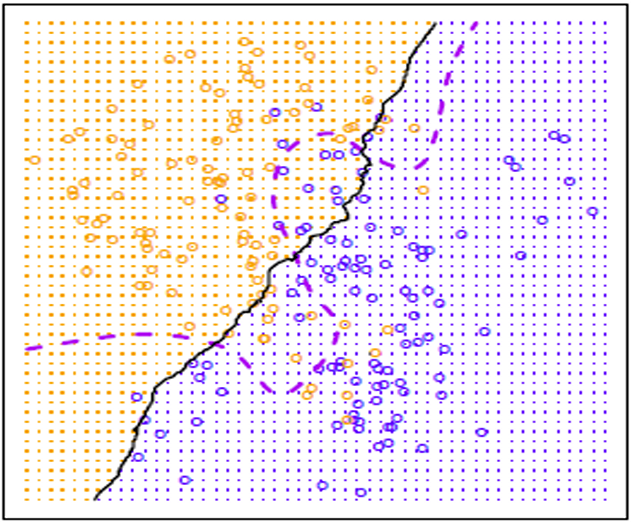
\includegraphics[width=.82\linewidth]{images/knn100.PNG}
        \caption{$k = 100$}
    \end{subfigure}
\caption{$k$-Nearest-Neighbor in two dimensions.}
\end{figure}

\noindent
An important detail for nearest-neighbor classification is that continuous variables \textit{need} to be normalized (otherwise variables with bigger domains prevail).

\noindent
\\
The NN classifier can estimate complex class borders locally and differently for each new instance, provides good generalization on many domains, learns quickly, is robust to noisy training data, and is easy to understand.
In contrast, it suffers a lot from irrelevant variables (the \textit{curse of dimensionality}; see Figure \ref{fig:curse-of-dimensionality}), slow classification, reduced generalization with increased noise, and has a large storage requirement.

\begin{figure}[h]
    \centering
    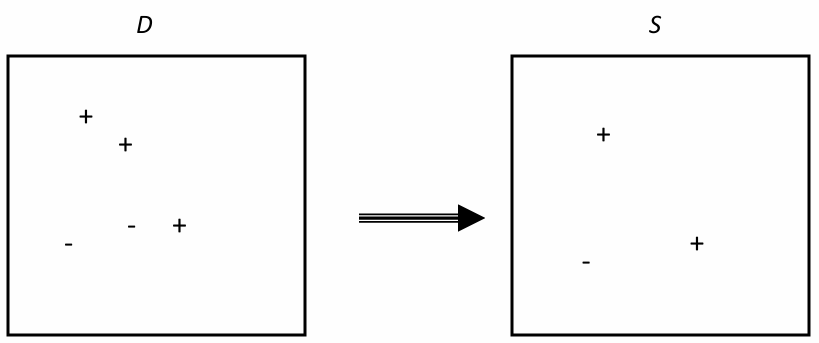
\includegraphics[scale=0.5]{images/condensed-nn.PNG}
    \caption{The \textbf{Condensed Nearest-Neighbor Algorithm} (CNN) was introduced to address the large storage requirements. This algorithm finds a subset $S$ of the training data $D$ such that each instance can be correctly classified using only $S$, usually resulting in a $60\%-80\%$ reduction in storage. A CNN classifier starts by randomly selecting one instance of every class and putting it in $S$. Each time an instance in $D$ is not correctly classified, it is added to $S$. This process is repeated until all instances in $D$ are correctly classified. The CNN algorithm is very sensitive to noise.}
\end{figure}

\noindent
A variation of CNN is the \textbf{Edited Nearest-Neighbor Algorithm} (ENN), a classifier proposed to stabilize NN accuracy when there is noise in the training data, usually resulting in a reduction of $20\%-40\%$.
The algorithm starts with the set $S$ equal to the training data $D$, and removes each instance $s \in S$ that does not agree with the majority of its $k$ nearest neighbors (usually $k = 3$).
This algorithm removes noisy instances as well as border cases, leading to overall smoother decision boundaries while not reducing the space as much as other reduction algorithms.

\noindent
\\
NN classifiers can be combined with decision trees in the form of \textit{model trees}: classify instances at leaf nodes according to a NN classifier over the associated training instances.
A similar procedure can also be done for decision rules.

%
% Topic 5 - Validation
%
\newpage
\section{Validation}
\textbf{Validation} is an important step in the data mining pipeline.
It is needed to determine whether to employ the model (e.g. estimate the performance), or to further optimize the model (e.g. post-pruning trees).
A common way to evaluate \textit{classifiers} is using the \textbf{Confusion Matrix}:

\begin{table}[h]
    \centering
    \begin{tabular}{l|l|c|c|c}
        \multicolumn{2}{c}{}&\multicolumn{2}{c}{Predicted Class}&\\
        \cline{3-4}
        \multicolumn{2}{c|}{}&Positive&Negative&\multicolumn{1}{c}{Total}\\
        \cline{2-4}
        \multirow{2}{*}{Actual Class}& Positive & $TP$ & $FN$ & $P$\\
        \cline{2-4}
        & Negative & $FP$ & $TN$ & $N$\\
        \cline{2-4}
    \end{tabular}
\end{table}

\noindent
Using this matrix we can calculate metrics such as \textbf{Accuracy}: $\frac{TP + TN}{P + N}$, \textbf{Error}: $\frac{FP + FN}{P + N}$, \textbf{Precision}: $\frac{TP}{TP + FP}$, \textbf{TP-Rate} (or \textbf{Recall}): $\frac{TP}{P}$, and \textbf{FP-Rate}: $\frac{FP}{N}$.

\subsection{Estimating Metrics} \label{sec:estim-metrics}
\noindent
We could estimate these metrics using the \textit{training data}, but they would not be good indicators of performance on future data (they only measure the degree of overfitting).
A more reliable way of estimating performance is to use independent \textit{testing data} (e.g. train on data from one year, test on data from another).
If a clear divide between training and testing data is not possible you can use the \textbf{Hold-Out Method}: split the data into a training and testing set (usually 80/20), train the model on the training data and evaluate it on the testing data.
This is an example of \textbf{Stratification}: the class distribution in the original data is preserved in both sets, reducing the estimate's variance.
An important note is that the hold-out method is \textit{unstable}:

\begin{itemize}
    \item Given a fixed \textit{test} set, the \textit{bias} decreases with the size of the \textit{training} data.
    \item Given a fixed \textit{training} set, the \textit{variance} decreases with the size of the \textit{test} data.
\end{itemize}

\noindent
To reduce the variance, the hold-out method has to be repeated multiple times with the performance metrics averaged.
The problem with repeating the hold-out method is that different training sets overlap with each other, as do different testing sets (i.e. some instances are only used for training, some only for testing).

\begin{figure}[h!]
    \centering
    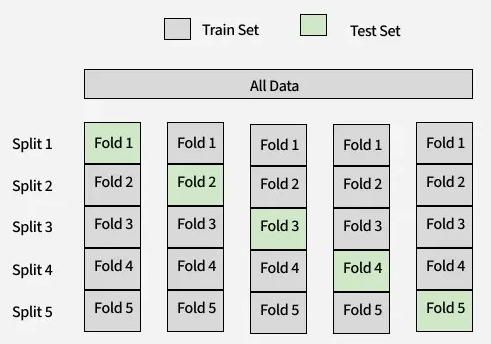
\includegraphics[scale=0.55]{images/kfold.png}
    \caption{\textbf{$k$-Fold Cross-Validation} avoids these overlapping test sets: \textbf{(1)} data is split into $k$ subsets of equal size. \textbf{(2)} each subset is used once for testing, the remaining are used for training. 10-fold cross-validation is a common validation method in practice, as $k=10$ seems to have the best bias-variance trade-off for estimating performance metrics.}
\end{figure}

\newpage
\noindent
A special case of $k$-fold cross-validation is \textbf{Leave-One-Out Cross-Validation}: $k$ is equal to the number of instances $n$.
This makes the best use of the data, involves no random sub-sampling, but is very computationally expensive and cannot be stratified.

\noindent
\\
It is important to note that cross-validation uses sampling \textit{without} replacement.
The \textbf{Bootstrap Method} uses sampling \textit{with} replacement:

\begin{enumerate}
    \item Sample a training set of $n$ instances (with replacement) from the original dataset (of size $n$).
    \item Use the instances from the original dataset that did \textit{not} get sampled as the testing set.
\end{enumerate}

\noindent
The bootstrap method is sometimes also called the \textbf{0.632 Bootstrap}, as this is the probability of a sample ending up in the training set:
\[ P(\text{test}) = \left( 1 - \frac{1}{n} \right)^n \approx e^{-1} = 0.368... \]

\noindent
This means the training data will contain roughly $63.2\%$ of the instances and the testing data will contain roughly $36.8\%$ of the instances.
Since the model is only trained on $63.2\%$ of the instances, the error estimate on the test data can often be very pessimistic.
A common way to adjust for this is by combing the training and testing error, and averaging over multiple samples:
\[ Error = 0.632 \cdot Error_{test} + 0.368 \cdot Error_{train} \]

\noindent
We can also estimate \textbf{Confidence Intervals} over metrics such as accuracy.
An overview of this can be found in Appendix \ref{app:conf}.
In summary: use the hold-out method for large datasets, use cross-validation for middle-sized datasets, use leave-one-out or the bootstrap method for small datasets.

\begin{figure}[h]
    \centering
    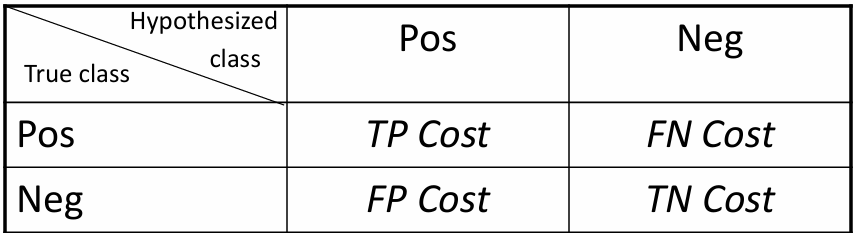
\includegraphics[scale=0.5]{images/costlearning.PNG}
    \caption{In practice, different types of classification errors often incur different \textit{costs}. If the classifier outputs probabilities for each class, it can be adjusted to minimize the \textit{expected cost}: the dot product between the class probabilities and the \textbf{Cost Matrix}, choosing the class with the lowest cost. \textbf{Cost Sensitive Learning} takes costs into account by resampling and weighting instances accordingly.}
\end{figure}

\noindent
Never use testing data for parameter tuning or feature selection: use a \textbf{Validation Set} instead (the model is build on the training plus validation data, and tested using the testing data).
\textbf{Data leakage} in validation occurs when information from outside the training fold is used (directly or indirectly) during model training or preprocessing, causing the model to appear more accurate than it really is.
Data leakage is "peeking" at the test data earlier in the pipeline, leading to optimistically-biased performance metrics and poor generalization to \textit{actual} unseen data.

\newpage
\subsection{ROC-Curve Analysis}
\begin{figure}[h]
    \centering
    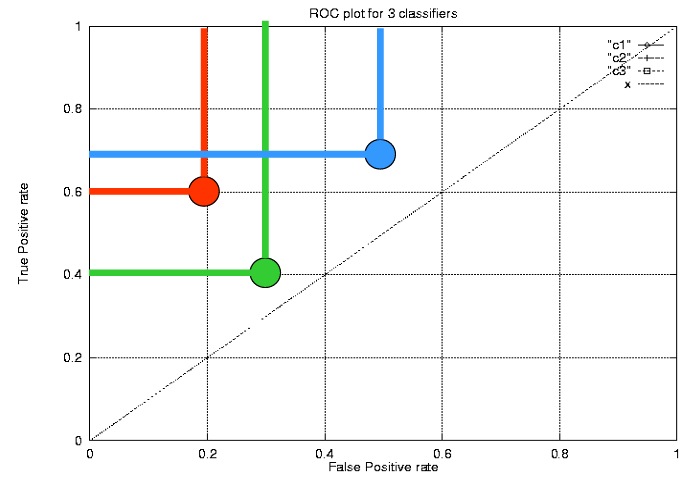
\includegraphics[scale=0.6]{images/roc-dominance.PNG}
    \caption{An \textbf{ROC-Curve} plots the TP-rate against the FP-rate of a classifier for various classification thresholds. A classifier that always predicts \textit{positive} will end up in the top-right corner, a classifier that always predicts \textit{negative} will end up in the lower-left corner. The straight line in the middle represents the performance of a random classifier. A classifier \textit{dominates} another classifier if and only if its TP-rate is higher and its FP-rate is lower (e.g. red dominates green).}
\end{figure}

\begin{figure}[h]
    \centering
    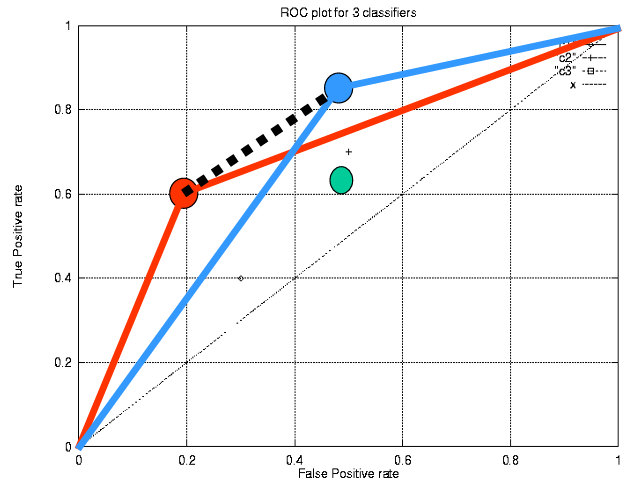
\includegraphics[scale=0.6]{images/rocch.PNG}
    \caption{The \textbf{ROC Convex Hull (ROCCH)} is a convex line connecting all \textit{dominant} classifiers. Classifiers lying on this line achieve the best accuracy, while classifiers lying below are sub-optimal. Any performance on a line segment connecting two ROC points can be achieved by randomly choosing between the respective classifiers.}
\end{figure}

\noindent
The standard procedure for constructing an ROC-curve for a probabilistic classifier is as follows:

\begin{enumerate}
    \item Define a \textit{discrete} classifier $h_t$ that predicts positive if $P_{pos} \geq t$.
    \item Compute the confusion matrix and plot the TP-rate and FP-rate of $h_t$.
    \item Repeat for each threshold $t \in [0, 1]$.
\end{enumerate}

\newpage
\begin{figure}[h]
    \centering
    \begin{subfigure}{.5\textwidth}
        \centering
        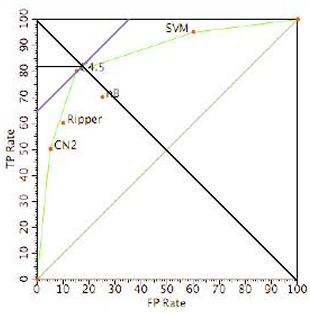
\includegraphics[width=.5\linewidth]{images/iso1.PNG}
        \caption{"C4.5" achieves around 82\% accuracy.}
    \end{subfigure}%
    \begin{subfigure}{.5\textwidth}
        \centering
        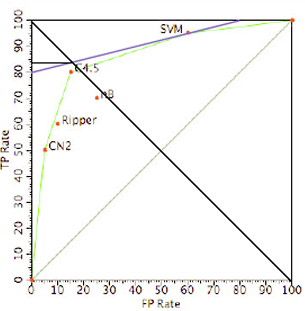
\includegraphics[width=.5\linewidth]{images/iso2.PNG}
        \caption{"SVM" achieves around 84\% accuracy.}
    \end{subfigure}
\caption{\textbf{Iso-Accuracy Lines} connect ROC points with the same accuracy $A$: $TPr = \frac{N}{P}FPr + \frac{A(P + N) - N}{P}$. Iso-accuracy lines have a slope of $\frac{N}{P}$ and lie tangent to ROC points.}
\end{figure}

\begin{figure}[h]
    \centering
    \begin{subfigure}{.33\textwidth}
        \centering
        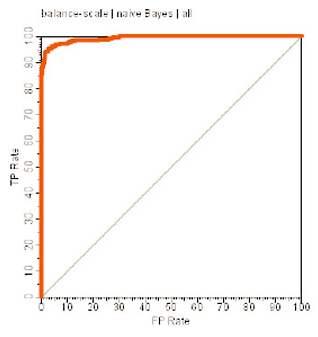
\includegraphics[width=.8\linewidth]{images/roc1.PNG}
        \caption{Good separation, convex.}
    \end{subfigure}%
    \begin{subfigure}{.33\textwidth}
        \centering
        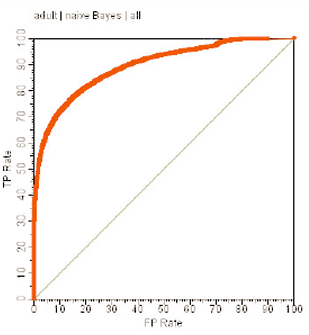
\includegraphics[width=.785\linewidth]{images/roc2.PNG}
        \caption{Reasonable separation, convex.}
    \end{subfigure}%
    \begin{subfigure}{.33\textwidth}
        \centering
        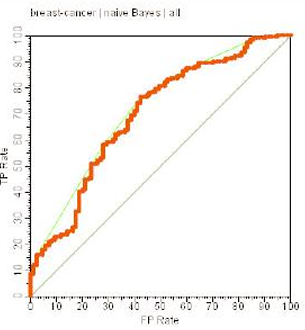
\includegraphics[width=.82\linewidth]{images/roc3.PNG}
        \caption{Poor separation, concave.}
    \end{subfigure}
\caption{Example ROC-curves for a single classifier.}
\end{figure}

\noindent
ROC-curves for probabilistic classifiers can also be constructed more efficiently:

\begin{enumerate}
    \item Sort test instances in decreasing order of probability of being classified as positive by \textit{probabilistic} classifier $h$.
    \item For each consecutive instance $x$: set the threshold $t$ equal to $P_{pos}(x)$, compute and plot the TP-rate and FP-rate of \textit{discrete} classifier $h_t$.
\end{enumerate}

\noindent
The \textbf{ROC AUC} metric is an estimation of the probability that a randomly chosen positive instance will be given a higher $P_{pos}$ than a randomly chosen negative instance.
It is equal to the area under the ROC-curve over the total area of the plot ($N \cdot P$).
A higher AUC value (closer to 1) indicates a better classifier, while an AUC value of 0.5 indicates a performance no better than a random classifier.

%
% Topic 6 - Feature Selection
%
\newpage
\section{Feature Selection}
Given a supervised learning task, \textbf{Feature Selection} is a process of selecting (a subset of) features such that the generalization performance of the predictive model is improved (feature selection generally leads to lower variance).
The main goals of feature selection include:

\begin{itemize}
    \item Avoid overfitting and improve generalization performance.
    \item Provide faster and more cost-effective models.
    \item Gain a deeper understanding of the underlying process that generated the data.
\end{itemize}

\noindent
In the Bayesian view, a feature $X_i$ is \textit{relevant} if and only if:
\begin{align*}
    P(Y | X) &\neq P(Y | X \backslash \{ X_i \}) && \text{(\textbf{Strong Relevance})} \\
    \exists Z \subseteq X \text{ s.t. } X_i \in Z \text{ and } P(Y | Z) &\neq P(Y | Z \backslash \{ X_i \}) && \text{(\textbf{Weak Relevance})}
\end{align*}

\begin{figure}[h!]
    \centering
    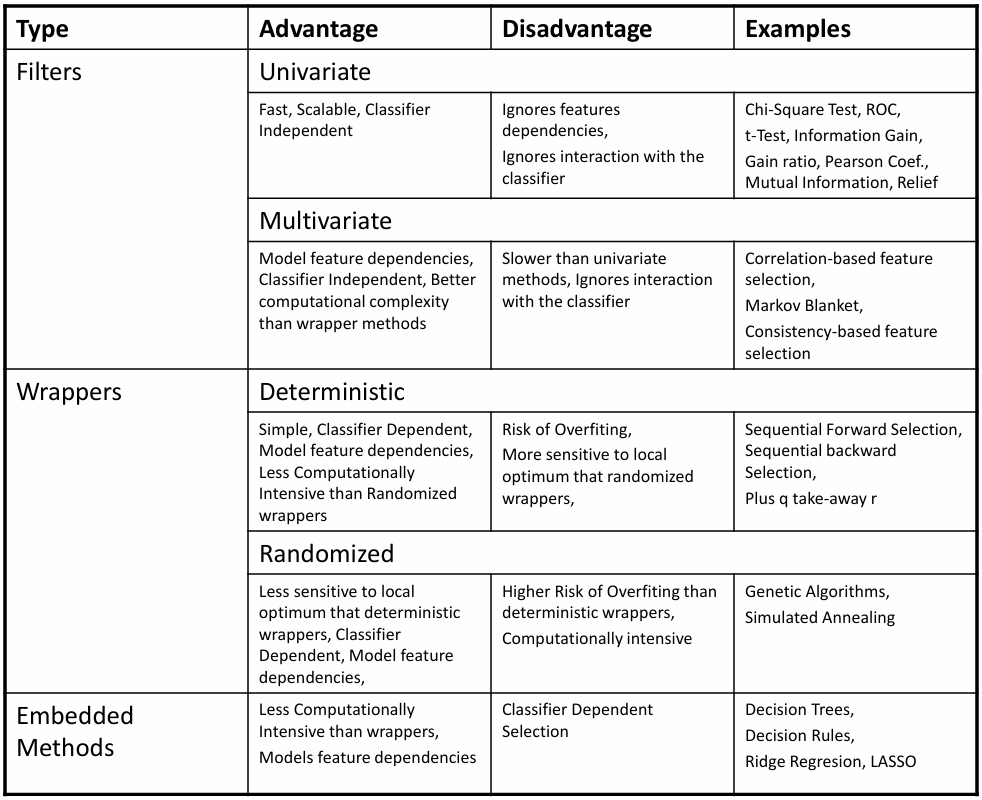
\includegraphics[scale=0.8]{images/feature-selection.PNG}
    \caption{Different types of feature selection.}
\end{figure}

\newpage
\subsection{Filters}
\textbf{Filters} rank (subsets of) features independently of the predictor.
There exist two types of filters: \textbf{Univariate} (produce feature scores) and \textbf{Multivariate} (produce feature-subset scores).

\subsubsection{Univariate Filters}
\noindent
The relevance of an individual feature $X_i$ is determined by how much $X_i$ can explain the output feature $Y$.
Statistically, this means that we need to assess the (in)dependence of $X_i$ and $Y$:

\begin{itemize}
    \item \textit{$X_i$ and $Y$ are both discrete}: \textbf{Chi-Squared Test} (see Section \ref{sec:integration}), \textbf{ROC Analysis} (threshold on $X_i$, AUC $= 0.5$ if $X_i$ and $Y$ are independent, $> 0.5$ if they are positively correlated, $< 0.5$ if they are negatively correlated), \textbf{Information Gain and Ratio} (see Section \ref{sec:decision-trees}), \textbf{Relief} (see Figure \ref{fig:relief}), \textbf{Mutual Information} (see below).
    \item \textit{$X_i$ is continuous, $Y$ is discrete}: \textbf{ROC Analysis} (see above), \textbf{Relief} (see Figure \ref{fig:relief}), \textbf{$t$-Test on Two Means} (assume $P(X_i | Y = -1)$ and $P(X_i | Y = 1)$ are Normal distributions with the same unknown variance $\sigma^2$, $t$-test on whether $\mu^+ = \mu^-$, see Appendix \ref{app:conf}).
    \item \textit{$X_i$ and $Y$ are both continuous}: \textbf{Mutual Information} (see below), \textbf{Pearson Correlation Coefficient} ($r = \left( \sum_{i = 1}^n (x_i - \bar{x})(y_i - \bar{y}) \right) / \left( \sqrt{\sum_{i = 1}^n (x_i - \bar{x})^2} \sqrt{\sum_{i = 1}^n (y_i - \bar{y})^2} \right)$, where 0 indicates independence, $< 0$ indicates negative correlation and $> 0$ indicates positive correlation, be aware that $r$ only catches \textit{linear} correlation, see Figure \ref{fig:correlation}).
\end{itemize}

\begin{figure}[h]
    \centering
    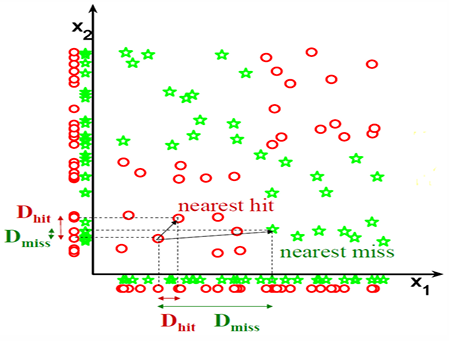
\includegraphics[scale=0.75]{images/relief.PNG}
    \caption{The \textbf{Relief Score} $W_i$ of a feature $X_i$ with respect to the output feature $Y$ is calculated as follows: \textbf{(1)} $W_i = 0$. \textbf{(2)} for all instances, $W_i = W_i + (D_{miss} - D_{hit})$, where $D_{miss}$ is the distance to the closest instance of the opposite class (\textbf{Near-Miss Distance}) and $D_{hit}$ is the distance to the closest instance of the same class (\textbf{Near-Hit Distance}).\label{fig:relief}}
\end{figure}

\noindent
\textbf{Mutual Information} quantifies the amount of information obtained about one variable by observing the other.
$MI(X_i, Y) = 0$ implies independence, $MI(X_i, Y) > 0$ implies (possibly \textit{non-linear}) dependence.
If $X_i$ and $Y$ are both \textit{discrete} or \textit{continuous}:
\[ MI(X, Y) = \sum_{y \in Y} \sum_{x \in X} P_{(X, Y)}(x, y) \log \left( \frac{P_{(X, Y)}(x, y)}{P_X(x) P_Y(y)} \right)\]
\[ MI(X, Y) = \int_Y \int_X P_{(X, Y)}(x, y) \log \left( \frac{P_{(X, Y)}(x, y)}{P_X(x) P_Y(y)} \right) dx dy\]

\newpage
\subsubsection{Multivariate Filters}
\begin{figure}[h]
    \centering
    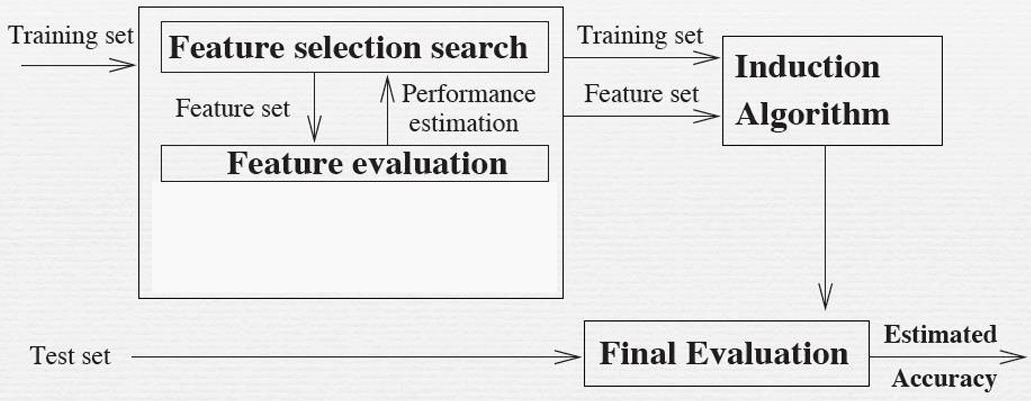
\includegraphics[scale=0.75]{images/multivariate-filter.PNG}
    \caption{\textit{Multivariate} filters search in the space of possible feature-subsets ($2^N$ combinations!).}
\end{figure}

\begin{figure}[h]
    \centering
    \begin{subfigure}{.5\textwidth}
        \centering
        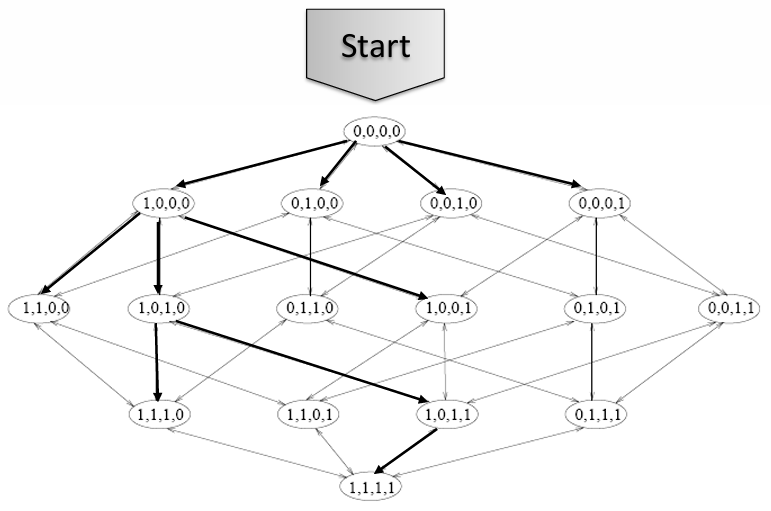
\includegraphics[width=.8\linewidth]{images/forward-selection.PNG}
        \caption{\textbf{Sequential Forward Selection (SFS)}:\\start with no features, add one at a time.}
    \end{subfigure}%
    \begin{subfigure}{.5\textwidth}
        \centering
        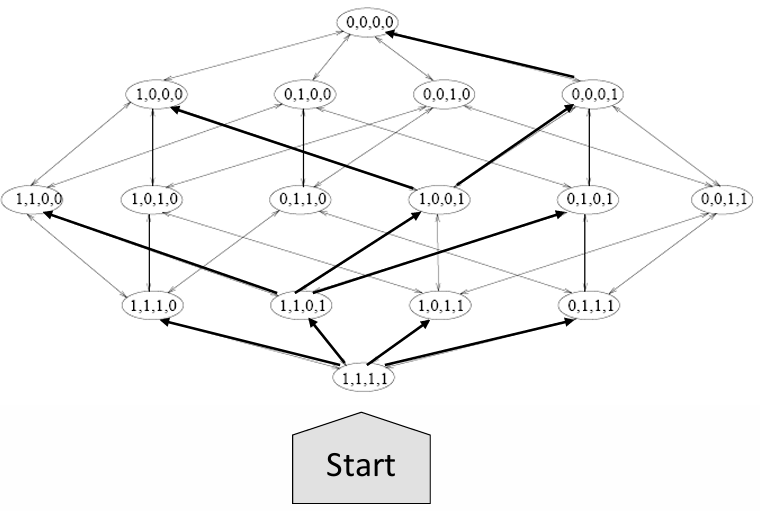
\includegraphics[width=.8\linewidth]{images/backward-selection.PNG}
        \caption{\textbf{Sequential Backward Selection (SBS)}:\\start with all features, remove one at a time.}
    \end{subfigure}
\caption{Possible ways of searching through the feature-subset space. Possible variations include \textbf{Bi-Directional Search}, \textbf{Floating Search} ($q$ steps of SFS, $r$ steps of SBS, repeat), etc.}
\end{figure}

\noindent
Other ways of searching for the optimal feature-subset include \textbf{Genetic Search} and \textbf{Hill Climbing}:

\begin{enumerate}
    \item Let $v$ be the initial state.
    \item Let $v^\prime$ be the child of $v$ that has the highest value for the evaluation function $f$.
    \item If $f(v^\prime) > f(v)$, then repeat the process for $v^\prime$.
\end{enumerate}

\noindent
Another similar approach is \textbf{Best-First Search}:

\begin{enumerate}
    \item Let $V$ be a list containing only the initial state.
    \item While $V$ is not empty: remove the best node $v \in V$, add its children to $V$, continue until $f(v)$ reaches some threshold.
\end{enumerate}

\newpage
\noindent
The \textbf{FOCUS} filter finds a minimal feature-subset $Z \subseteq X$ such that there are no two instance $(x_i, y_i)$, $(x_j, y_j)$ where $x_i = x_j$ and $y_i \neq y_j$.
Traditionally this would be done by simply searching over all possible subsets, but some extensions of the algorithm exist that use a heuristic search.

\noindent
\\
The final multivariate filter discussed here is \textbf{Correlation-Based Feature Selection}.
This means evaluation of a feature-subset is done according to the following formula:
\[ CFS(X) = \frac{|X| \cdot r_{cf}}{\sqrt{|X| + (|X| - 1) \cdot r_{ff}}} \]

\noindent
Where $X$ is a feature-subset with $|X|$ features, $r_{cf}$ is the average correlation between the features in $X$ and the class feature $Y$, and $r_{ff}$ is the average correlation between the features in $X$.

\subsection{Wrappers}
\textbf{Wrappers} rank feature-subsets with respect to the predictor used.
Similarly to filters, wrappers search the feature-subsets space and choose the subsets that maximize an evaluation criterion based on the predictor used (since they have the same hypothesis space, wrappers use the same search algorithms as multivariate filters).
The main downside of wrappers is that they are very slow compared to other feature selection methods.

\noindent
\\
One of the most popular wrappers (also one of the first) is \textbf{Recursive Feature Elimination (RFE)}: a wrapper that recursively reduces the set of features by eliminating the least important ones:

\begin{enumerate}
    \item Let $X$ be the initial set of features and let $k$ be the \textit{desired} size of $X$.
    \item Train model $h$ on representation $X$.
    \item Let $h$ assign a rank $r$ to each variable $x \in X$.
    \item Validate model $h$ to obtain a performance measure value $P$. If this value is lower than in the previous iteration, then stop.
    \item Eliminate variable $x$ with the lowest rank $r$ and repeat while $|X| > k$.
\end{enumerate}

\noindent
Advantages of RFE include the fact that it takes feature dependencies into account (assuming this is incorporated in the variable ranking), it can identify correlated features, and it can be used with any model that assigns importance to features.
Limitations of RFE include its computational complexity (training the model many times), and its dependence on the base model chosen.
For \textit{parametric} models, feature ranking is determined using the absolute values of parameters.
For nearest-neighbor models, features can be ranked using relief scores.
In the context of tree models, features can be ranked using \textbf{Variable Importance}:
\[ I(x) = \sum_{\text{node } n} \text{proportion of instances in } n \times \text{Impurity Gain of } x \text{ in } n \]

\subsection{Embedded Methods}
\textbf{Embedded Methods} are all the learning methods that derive \textit{white box} predictors (e.g. decision trees, decision rules, ridge regression, lasso regression, etc.).
This often leads to more direct search than e.g. wrappers.

%
% Topic 7 - Ensembles
%
\newpage
\section{Ensembles}
The basic idea of \textbf{Ensembles} is to learn a \textit{set} of models and allow them to vote on the final prediction.
This has the advantage of generally improving accuracy, while the disadvantage is that it makes the models harder to understand.
Ensembles overcome three problems:

\begin{itemize}
    \item The \textbf{Statistical Problem} that arises when the hypothesis space is too large for the amount of available data. This leads to multiple hypotheses having the same accuracy while the learning algorithm chooses only one of them (possibly one that performs worse on unseen data).
    \item The \textbf{Computational Problem} that arises when the learning algorithm cannot guarantee to find the best hypothesis (this and the statistical problem lead to the \textit{variance} component of the error).
    \item The \textbf{Representational Problem} that arises when the hypothesis space does not contain any good approximation of the target classes (this leads to the \textit{bias} component of the error).
\end{itemize}

\subsection{Independently Constructing Ensembles}
One way to force a learning algorithm to construct multiple hypotheses is to run the algorithm several times with somewhat different data in each run.

\subsubsection{Majority Vote}
\textbf{Majority Vote} is the simplest way of constructing ensembles.
The idea is to build multiple, slightly different models and have them decide the final prediction through a majority vote.
Consider a majority vote classifier consisting of 25 base models: if each base model has an (\textit{assumed independent}) error rate of $\epsilon = 0.35$, then the probability of the ensemble classifier making an incorrect prediction is given by:
\[ P(X \geq 13) = \sum_{i = 13}^{25} \binom{25}{i} \epsilon^i (1 - \epsilon)^{25 - i} \approx 0.06 \]

\noindent
Since the variance of the mean of multiple observations is given by $\frac{\sigma^2}{n}$, majority voting mostly reduces the \textit{variance error} component of the classifiers. 
The big problem in ensemble learning is that the \textit{independent error} assumption is very unrealistic.
The main (active) research question in ensemble learning is how to make the error of each classifier as independent as possible.

\begin{figure}[h!]
    \centering
    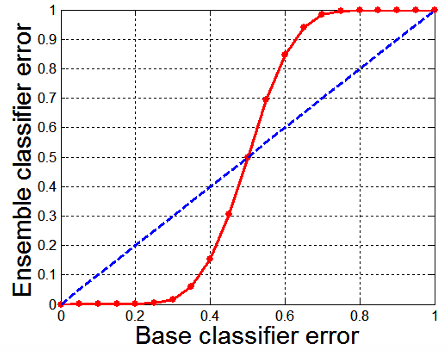
\includegraphics[scale=0.7]{images/majority-vote.PNG}
    \caption{How the ensemble classifier error scales with the base classifier error.}
\end{figure}

\newpage
\subsubsection{Bagging}
\textbf{Bagging} is a very common variant of majority vote: training each base classifier on a \textit{bootstrap sample} (see Section \ref{sec:estim-metrics}) of the data.
A common classifier used with bagging is \textit{decision trees}, resulting in smoother decision boundaries than a single decision tree would produce.
This smoother decision boundary can slightly decrease the bias, but bias can also slightly increase due to the less informative data subsets.

\noindent
\\
The remaining data not used to train each base classifier is called the \textbf{Out-of-Bag (OOB)} instances.
To validate a bagging ensemble we can predict the response for the $i$th instance using each of the classifiers for which that instance was OOB, yielding around $\frac{t}{3}$ predictions (where $t$ is the number of base classifiers) that can be averaged to predict the $i$th instance.
If $t$ is sufficiently large, this estimate is essentially the leave-one-out cross-validation error for bagging.

\subsubsection{Random Forest}
\textbf{Random Forest} is a variation of bagging that uses \textit{random} trees to increase the independence of the base classifier errors.
Where normal bagging builds optimal decision trees, random forests build decision trees where at each node only a random subset of $m$ features is considered ($m$ is usually around $\sqrt{M}$, can be fine-tuned using OOB validation).
Random forests usually show no further improvement after around 100 trees.

\noindent
\\
Since random forest is a bagging method, it reduces error by reducing the variance through majority voting.
Bias can slightly increase due to the less competent bagged classifiers, or slightly decrease due to the smoother decision boundary.
Random forests usually outperform bagging due to the errors of the decision trees being less correlated.

\noindent
\\
Both bagging and random forests can be easily adapted for regression problems: instead of majority vote, the final prediction is assembled by \textit{averaging} over the base predictions.
Similarly to classification, this works best with regression models that have a high variance component (higher \textit{flexibility}).

\begin{figure}[h!]
    \centering
    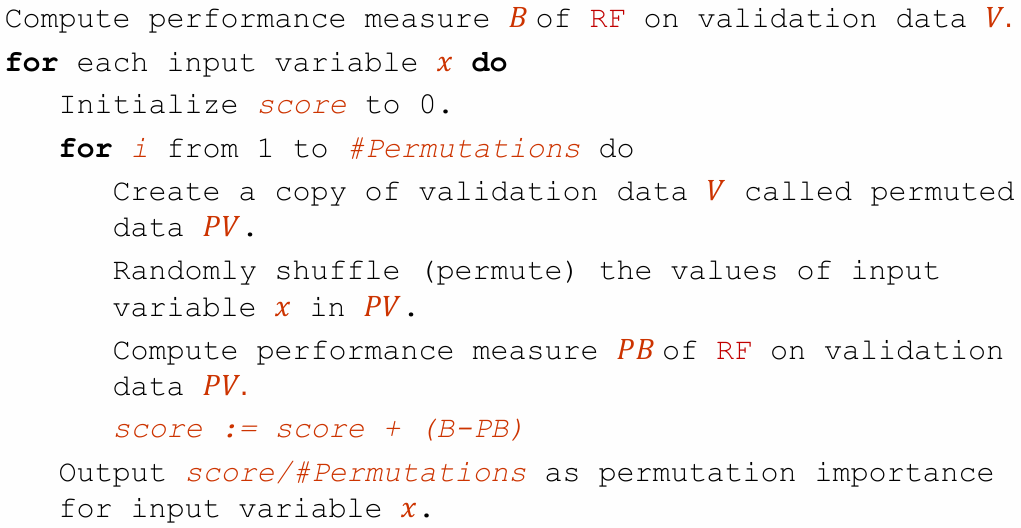
\includegraphics[scale=0.65]{images/permutation-importance.PNG}
    \caption{\textbf{Permutation Importance} in random forests, assessing the significance of each feature.}
\end{figure}

\newpage
\subsubsection{Error-Correcting Output Codes (ECOC)}
\begin{figure}[h]
    \centering
    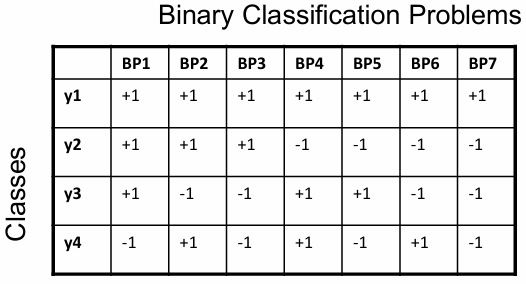
\includegraphics[scale=0.75]{images/ecoc.PNG}
    \caption{For $k$ number of classes we receive $2^{k-1}-1$ number of binary classification problems. For each of these problems we train a binary classifier. The predictions by the binary classifiers for a test instance form a \textit{"code word"} for that instance (e.g. $[+1, +1, -1, +1, -1, +1, -1]$). The final predicted class is the class with the code word closest to that of the test instance.\label{fig:ecoc}}
\end{figure}

\noindent
An ECOC matrix $M$ has to satisfy two properties:

\begin{itemize}
    \item \textbf{Row Separation}: any class code word in $M$ should be well-separated from all other class code words in $M$.
    \item \textbf{Column Separation}: any class-partition code word in $M$ should be well-separated from all other class-partition code words and their complements.
\end{itemize}

\noindent
For the example in Figure \ref{fig:ecoc} (\textit{Exhaustive ECOC}): the Hamming distance between class code words is $2^{k-2}$, the number of error corrections is $2^{k-3}-1$, and the minimal Hamming distance between class partition code words is 1.
Other examples of ECOC include \textit{One-Against-All} ($k$ binary classifiers, majority vote), \textit{One-Against-One} ($k(k-1)/2$ binary classifiers, majority vote), and \textit{Minimal Codes} ($\log_2 k$ binary classifiers, code word determines the class exactly; the problem is that an error of one of the binary classifiers would mean an error of the whole ensemble).

\subsection{Coordinated Constructing Ensembles}
The key idea of coordinated ensembles is that the classifiers are complementary, with instance classification through a weighted sum of the classifiers.

\subsubsection{Boosting}
\textbf{Boosting} is similar to majority vote, but models are weighted according to their performance.
Boosting works through an iterative procedure: new models are encouraged to become experts for instances classified incorrectly by earlier models.
It can also be applied without weights by resampling with probabilities.
Boosting decreases the training error exponentially in the number of iterations, and works well if the base classifiers are not too complex and their error does not grow too quickly.
Boosting reduces the bias component of the error of simple classifiers, as it creates a more complex model.
The most popular variant of boosting is \textbf{AdaBoost}:

\newpage
\begin{figure}[h]
    \centering
    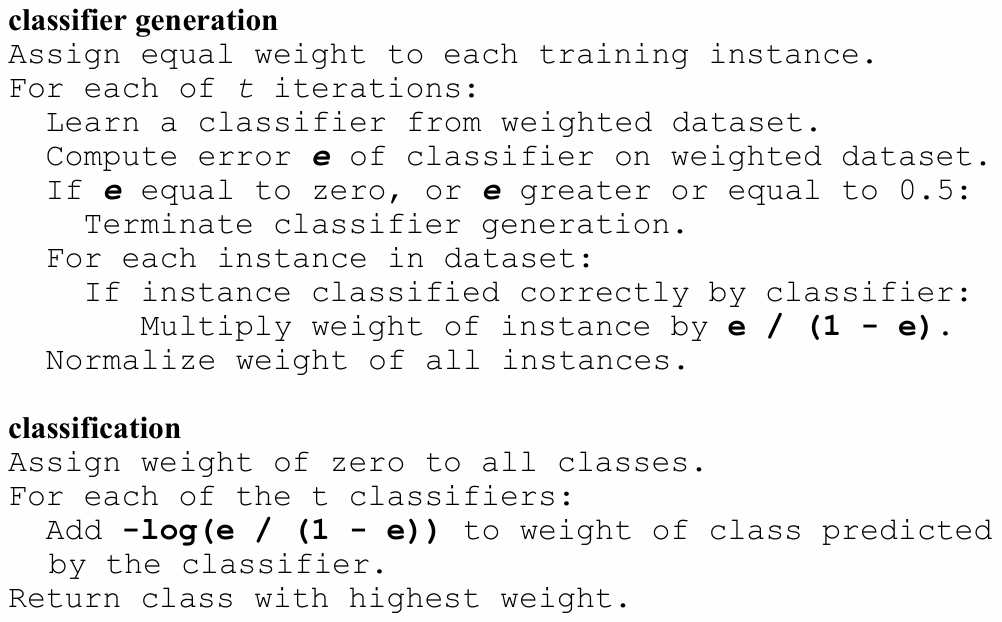
\includegraphics[scale=0.65]{images/adaboost.PNG}
    \caption{Pseudocode of \textbf{AdaBoost}.}
\end{figure}

\noindent
AdaBoost is also used in \textbf{Transfer Learning}: assume two classification tasks that have a different probability distribution $P(X, Y)$ (i.e. we cannot take data from the \textit{source} and use it to train the \textit{target}).
To solve this we can \textit{decrease} the weight of misclassified data from the source domain, and \textit{increase} the weight of misclassified data from the target domain.

\subsubsection{Stacking}
\textbf{Stacking} refers to the use of \textbf{Meta Learners} to combine predictions instead of voting.
Predictions of the base models (\textit{level 0 models}) are used as input for the meta learner (\textit{level 1 model}), usually using a different learning scheme.
If the base learners can output probabilities, it is better to use those as input to the meta learner.
The downside of stacking is that the resulting models are hard to theoretically analyze, resulting in \textit{black box} models.

\noindent
\\
Note that predictions from the level 0 classifiers on the training data \textit{cannot} be used as training data for the level 1 classifier (the level 1 model will simply choose the level 0 classifier that best fit the data).
Instead a $k$-fold cross-validation structure should be employed, with the predictions of the testing data acting as the training data for the level 1 classifier.

\noindent
\\
Meta learners can also be used for \textbf{Reliable Classification}: a form of classification where classifiers can also return a "$?$" symbol if they are unable to classify an instance correctly.
The instance is given to both a base classifier as well as a meta classifier, who determines whether to use the base classifier's prediction or not.
The \textit{precision} of the meta classifier is equal to the \textit{accuracy} of the combined classifier on the classified instances.

\noindent
\\
In summary, if the classifier is very \textit{flexible} (i.e. high \textit{variance}), then apply bagging.
If the classifier is \textit{inflexible} and \textit{simple} (i.e. high \textit{bias}), then apply boosting.
If you have many classes and a binary classifier, try ECOC.

\newpage
\subsection{Co-Training}
Given a set of labeled training instances $L$ and a set of unlabeled instances $U$, the \textbf{Co-Training} / \textbf{Self-Training} algorithm follows the following loop:

\begin{itemize}
    \item Learn a classifier $H$ from $L$.
    \item Let $H$ label $p$ positive and $n$ negative examples from $U$.
    \item Add these newly labelled instances to $L$.
\end{itemize}

\noindent
Co-training works when examples are described by \textit{redundantly sufficient features} and when the hypothesis spaces corresponding to the sets of redundantly sufficient features contain different hypotheses or the learning algorithms are different.

\begin{figure}[h]
    \centering
    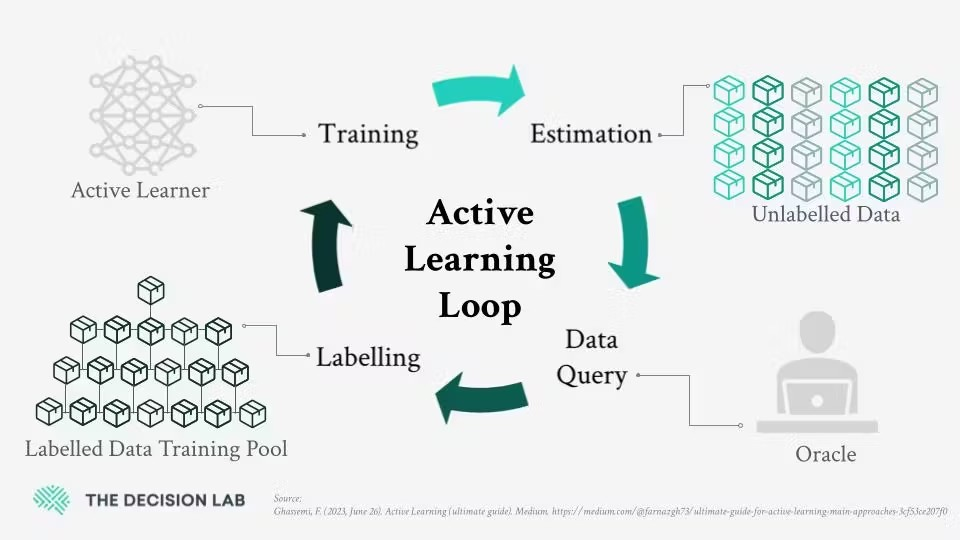
\includegraphics[scale=0.4]{images/active-learning.png}
    \caption{Labeled data is often expensive to obtain. \textbf{Active Learning} learns from a pool of unlabeled data by querying an \textit{oracle} (human) for labels. The goal of active learning is to achieve high accuracy while using as few labeled data as possible. The function that determines which instances to label is called a \textbf{Query Function}. Possible query functions include \textit{uncertainty sampling} (choose the least certain instance), \textit{version space reduction} (the subset of hypotheses consistent with the training data), and \textit{entropy reduction} (find the greatest reduction in the total number of incorrect predictions).}
\end{figure}

%
% Topic 8 - Clustering
%
\newpage
\section{Clustering}
A \textbf{Cluster} is a collection of data objects that are \textit{similar} to objects in the same group, and \textit{dissimilar} to objects in other groups (see Figure \ref{fig:cluster}).
\textbf{Cluster Analysis} (or \textit{clustering}, \textit{data segmentation}, etc.) is the process of finding (dis)similarities according to the characteristics found in the data and grouping similar objects into clusters.
The separation of clusters can be \textit{exclusive} (one instance belongs to one class) or \textit{non-exclusive} (one instance can belong to multiple classes).
Clustering is an example of \textit{unsupervised learning}, meaning there are no predefined classes to train on.
Typical applications of clustering include as a \textit{stand-alone tool} to get insights into the data distribution, or as a \textit{pre-processing} step for other algorithms.

\begin{figure}[h]
    \centering
    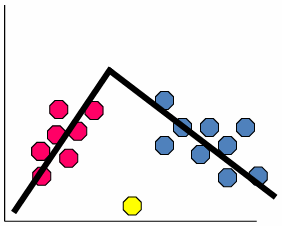
\includegraphics[scale=0.75]{images/cluster-application.PNG}
    \caption{Instead of applying linear regression over the whole dataset, it is independently applied to \textit{clusters} of the dataset. This turns linear regression from a \textit{global} model into a \textit{local} model. Similar applications include simplifying $k$-NN by using clusters instead of data points, or outlier detection (points far away from any cluster).}
\end{figure}

\subsection{Partition-Based Clustering}
A common approach to clustering is \textbf{Partitioning}: partitioning a database of $n$ objects into a set of $k$ clusters such that the sum of squared errors is minimized (where $c_i$ is the center of cluster $C_i$):
\[ SSE = \sum_{i = 1}^k \sum_{p \in C_i} dist(c_i, p)^2 \]

\noindent
Finding the global optimal through exhaustive search is NP-hard.
The most common heuristic approach to find a good set of clusters is \textbf{K-Means}:

\begin{enumerate}
    \item Partition objects into $k$ nonempty subsets at random.
    \item Compute the centers of the clusters.
    \item Assign each object to the cluster with the closest center.
    \item Repeat from step 2 until the partition does not change.
\end{enumerate}

\noindent
The main strength of K-means is it efficiency, running in linear time with respect to $n$, $k$, and the number of iterations $t$ (usually around 5-10).
The downsides are that it often terminates at a \textit{local} optimal, with it being very sensitive to the initial randomization.
It is also sensitive to noise and outliers, can only discover \textit{convex} clusters, and is limited by needing to specify $k$ in advance.

\newpage
\begin{figure}[h]
    \centering
    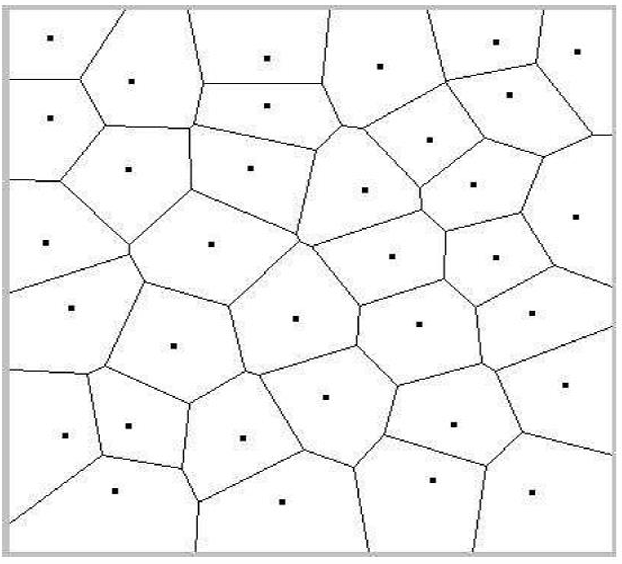
\includegraphics[scale=0.4]{images/convexity.PNG}
    \caption{K-means can only discover \textit{convex} clusters.}
\end{figure}

\noindent
While K-means can only cluster \textit{numeric} data, \textbf{K-Modes} can cluster \textit{categorical} data by using the \textit{mode} instead of the \textit{mean} of clusters.
Another variation of K-means is \textbf{K-Medoids} (or \textbf{Partition Around Medoids (PAM)}): instead of the mean, use the most centrally located object as center reference.
Since K-medoids uses \textit{representative objects} instead of the mean, it is less sensitive to outliers.
K-medoids works very well on small datasets, but does not scale well with large datasets due to the additional computational complexity.
\textbf{CLARA} is a clustering algorithm that uses K-medoids with \textit{sampling}, making it a lot more efficient (at the cost of higher variance).

\subsection{Hierarchical Clustering}
\textbf{Hierarchical Clustering} produces a set of nested clusters organized as a tree (each level of the tree represents one level of clusters)

\begin{figure}[h]
    \centering
    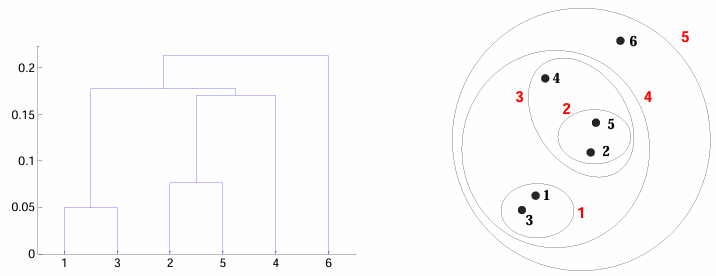
\includegraphics[scale=0.8]{images/hierarchical-clustering.PNG}
    \caption{Hierarchical clusters are usually visualized as a \textit{dendogram}, a tree-like diagram where the height at which clusters merge reflect the distance between the clusters.}
\end{figure}

\noindent
The strength of hierarchical clustering is that it does not assume any particular number of clusters: any number of clusters can be obtained by cutting the dendogram at a different level.
Some subtrees may even correspond to meaningful taxonomies (e.g. animal kingdom, biological structures, etc.).
The downside of this is that these dendograms grow very quickly with the number of instances, as each leaf is restricted to representing only a single instance.

\noindent
\\
The two main types of hierarchical clustering are \textbf{Agglomerative} (start with all points as individual clusters, merge until $k$ clusters are left) and \textbf{Divisive} (start with one cluster, split until clusters are of minimum size or there are $k$ of them).

\newpage
\subsubsection{Agglomerative Clustering}
The basic algorithm of agglomerative clustering is as follows:

\begin{enumerate}
    \item Compute the distance (or \textit{proximity}) matrix.
    \item Let each data point be its own cluster.
    \item Merge the two closest clusters and update the distance matrix, repeat until only a single cluster remains.
\end{enumerate}

\noindent
The key operation of agglomerative clustering is the computation of distance between clusters.
Different distance approaches lead to different clusters. 
Some popular distance measures include:

\begin{itemize}
    \item \textbf{MIN / Single Link}: distance between clusters is defined as the distance between the closest points. Single Link can handle clusters of any shape, but is more sensitive to noise and outliers.
    \item \textbf{MAX / Complete Link}: distance between clusters is defined as the distance between the most distant points. Complete Link is less susceptible to noise and outliers, but more biased towards global clusters.
    \item \textbf{Group Average}: distance between clusters is defined as the average pairwise distance between points in the clusters (average since it otherwise favours large clusters):
    \[ proximity(C_i, C_j) = \frac{\sum_{p_i \in C_i} \sum_{p_j \in C_j} proximity(p_i, p_j)}{|C_i| \cdot |C_j|} \]
    Group Average acts as a compromise between single and complete link, being less susceptible to outliers but more biased towards global clusters.
    \item \textbf{Centroid Distance}: distance between clusters is defined as the distance between the means of the clusters.
    \item \textbf{Ward's Method}: distance between clusters is defined as the increase in squared error when the clusters are merged (similar to group average with the distance between points squared). Ward's Method is less susceptible to noise and outliers, but more biased towards global clusters.
\end{itemize}

\begin{figure}[h!]
    \centering
    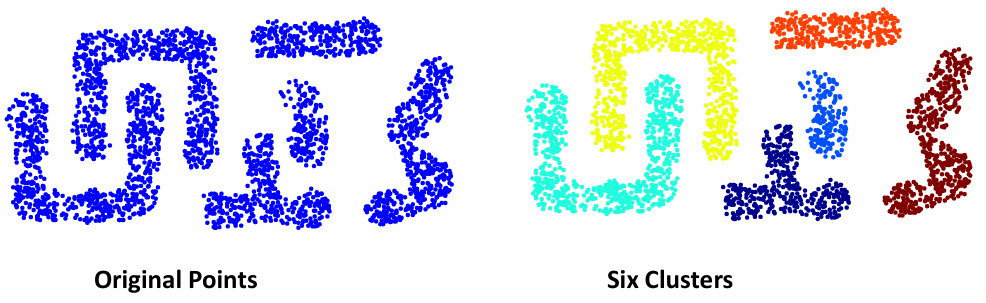
\includegraphics[scale=0.75]{images/clusters-min.PNG}
    \caption{\textit{MIN} can handle clusters of any shape.}
\end{figure}

\newpage
\begin{figure}[h]
    \centering
    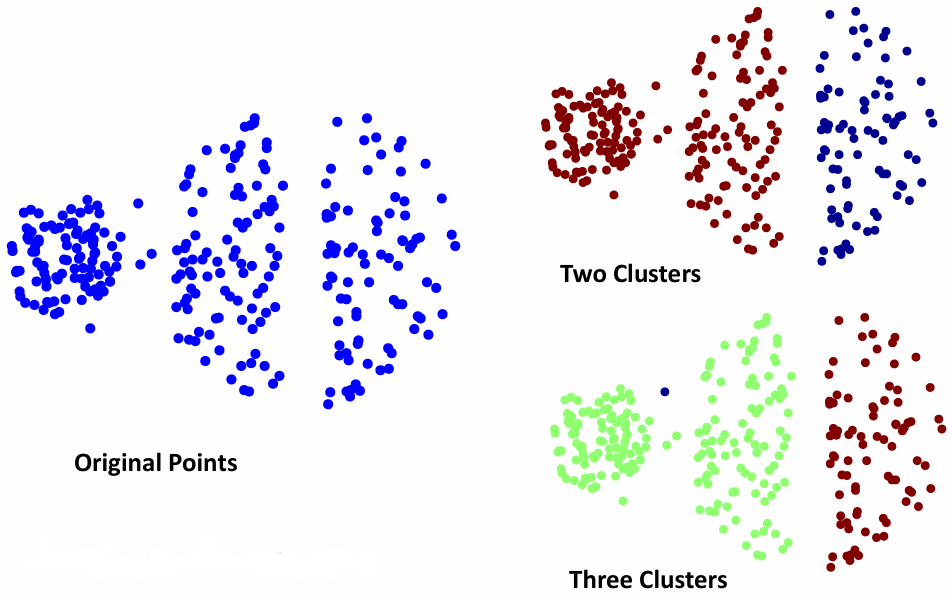
\includegraphics[scale=0.6]{images/clusters-outliers.PNG}
    \caption{A limitation of \textit{MIN} is that it is very sensitive to noise and outliers. However, this is not strictly a limitation. Thanks to its sensitivity to outliers, it is also easy to \textit{identify} outliers and prune them from the tree.}
\end{figure}

\begin{figure}[h!]
    \centering
    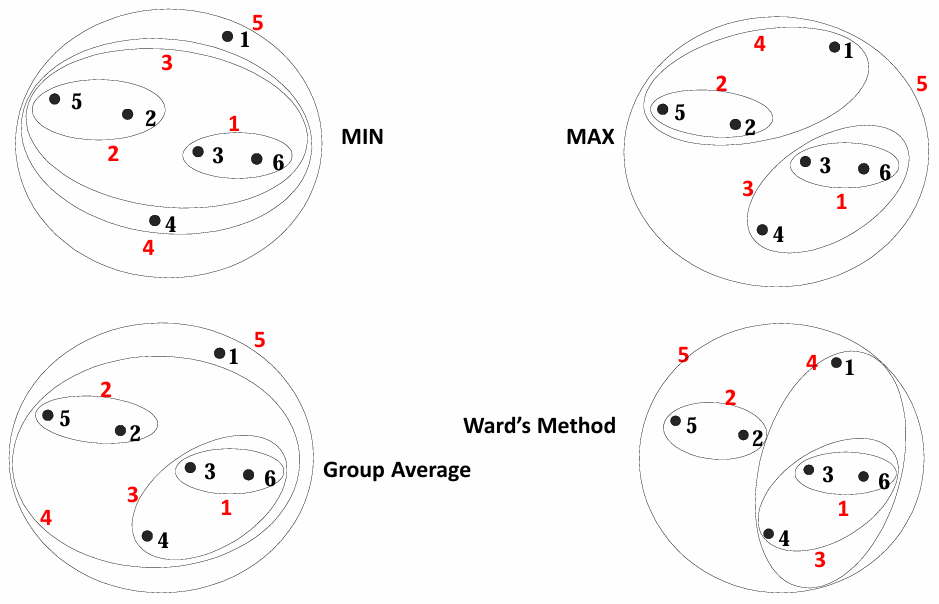
\includegraphics[scale=0.6]{images/clustering-methods.PNG}
    \caption{Hierarchical clustering with different distance measures. An "annoying" property of clustering is that the same algorithm on only six data points can achieve completely different sets of clusters depending on its parameters.}
\end{figure}

\subsubsection{CHAMELEON}
The \textbf{CHAMELEON} algorithm measures the similarity based on a dynamic model: two clusters are merged only if the \textit{interconnectivity} and \textit{closeness} between them are high relative to the internal interconnectivity and closeness of points within the clusters.

\newpage
\noindent
The \textbf{Relative Interconnectivity} between clusters $C_i$ and $C_j$ is the absolute interconnectivity between $C_i$ and $C_j$ normalized by the internal interconnectivity of $C_i$ and $C_j$:
\[ RI(C_i, C_j) = \frac{EC_{\{C_i, C_j\}}}{\frac{1}{2}(EC_{C_i} + EC_{C_j})} \]

\noindent
Where $EC_{\{C_i, C_j\}}$ is the sum of the edges connecting clusters $C_i$ and $C_j$, and $EC_{C_i}$ is the minimum sum of the cut edges that partition $C_i$ into two equal parts.

\noindent
\\
The \textbf{Relative Closeness} between clusters $C_i$ and $C_j$ is the absolute closeness between $C_i$ and $C_j$ normalized by the internal closeness of $C_i$ and $C_j$:
\[ RC(C_i, C_j) = \frac{S_{EC_{\{C_i, C_j\}}}}{\frac{|C_i|}{|C_i + C_j|} S_{EC_{C_i}} + \frac{|C_j|}{|C_i + C_j|} S_{EC_{C_j}}} \]

\noindent
Where $S_{EC_{\{C_i, C_j\}}}$ is the average weight of the edges that connect vertices in $C_i$ to vertices in $C_j$, and $S_{EC_{C_i}}$ is the average weight of the edges that partition $C_i$ into two equal parts.

\begin{figure}[h]
    \centering
    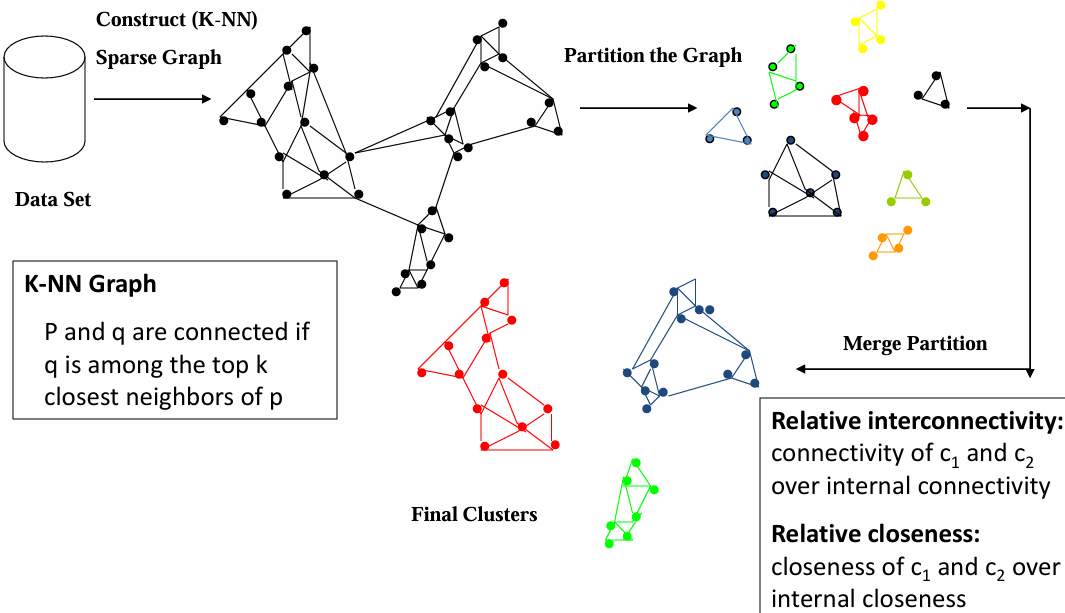
\includegraphics[scale=0.55]{images/chameleon.PNG}
    \caption{CHAMELEON is a two-phase algorithm: \textbf{(1)} use a graph-partitioning algorithm to cluster objects into a large number of relatively small sub-clusters. \textbf{(2)} use an agglomerative hierarchical clustering algorithm to find the genuine clusters by repeatedly combining these sub-clusters. Since hierarchical clustering algorithms are usually $O(n^2)$, CHAMELEON is not computationally efficient.}
\end{figure}

\begin{figure}[h!]
    \centering
    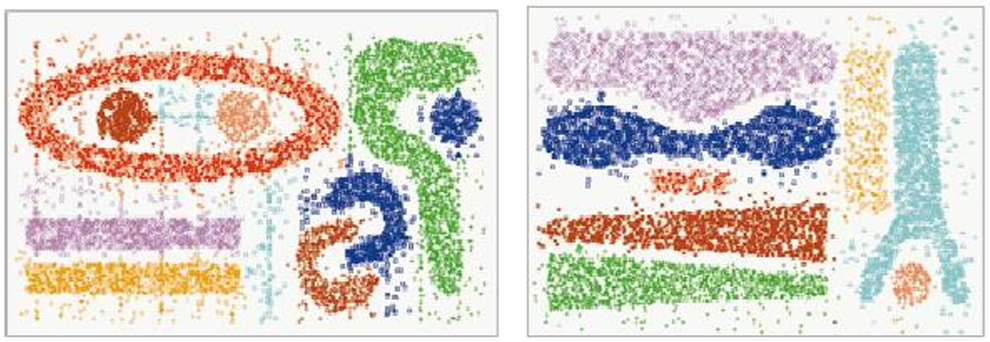
\includegraphics[scale=0.5]{images/chameleon-clusters.PNG}
    \caption{CHAMELEON can identify clusters of complex shapes.}
\end{figure}

\newpage
\subsection{Density-Based Clustering}
\textbf{Density-Based Clustering} identifies clusters based on \textit{density} (a local cluster criterion; e.g. density-connected points).
These algorithms generally have two parameters: $\epsilon$ (the maximum radius of the neighborhood), and \textit{minPts} (the minimum number of points in an $\epsilon$-neighborhood).
A point $p$ is \textbf{Directly Density-Reachable} from a point $q$ if $dist(p, q) \leq \epsilon$ and the number of points within $q$'s $\epsilon$-neighborhood is $\geq$ \textit{minPts}, a point $p$ is \textbf{Density-Reachable} from a point $q$ if there is a chain of directly density-reachable points from $q$ to $p$, and a point $p$ is \textbf{Density-Connected} to a point $q$ if there exists a point $o$ such that both $p$ and $q$ are density reachable from $o$.
A point is a \textbf{Core Point} if it has $\geq$ \textit{minPts} within $\epsilon$, a \textbf{Border Point} if it has $<$ \textit{minPts} within $\epsilon$, or a \textbf{Noise Point} if it is neither a core point or a border point.

\noindent
\\
The most popular density-based clustering algorithm is \textbf{Density-Based Spatial Clustering of Applications with Noise (DBSCAN)}.
DBSCAN relies on a density-based notion of clusters: a subset $C \subseteq D$ is a cluster if and only if \textbf{(1)} any two objects $o_1, o_2 \in C$ are density-connected, and \textbf{(2)} there does not exist an object $o \in C$ that is density-connected with some object $o^\prime \in D \backslash C$.
DBSCAN can discover clusters of arbitrary shapes in datasets with noise and outliers.
The downside of DBSCAN is that it is very sensitive to its parameters, with small changes in $\epsilon$ and \textit{minPts} leading to drastically different sets of clusters.

\begin{figure}[h]
    \centering
    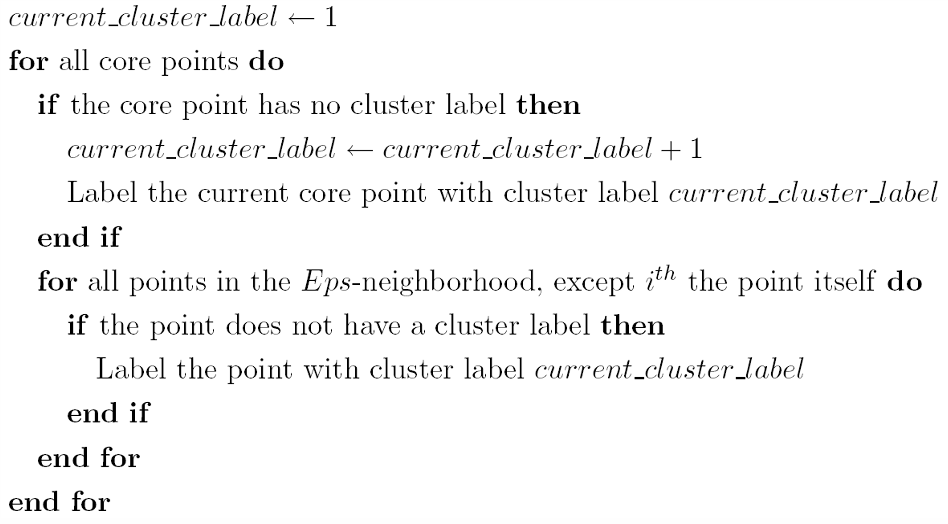
\includegraphics[scale=0.6]{images/dbscan.PNG}
    \caption{Pseudocode of DBSCAN.}
\end{figure}

\subsection{Grid-Based Clustering}
\textbf{Grid-Based Clustering} is a more efficient type of density-based clustering ($O(n)$):

\begin{enumerate}
    \item Define and fill in a set of grid cells representing \textit{density} (points per amount of space).
    \item Eliminate cells having a density below some threshold $t$.
    \item Form clusters from adjacent groups of dense cells.
\end{enumerate}

\noindent
Cells can be defined using \textit{equal-width}, \textit{equal-frequency}, or \textit{variable-range} bins.

\newpage
\subsection{Evaluation of Clusters}
We would like to evaluate clusters to avoid finding patterns in noise, or compare different algorithms or sets of clusters.
Unlike \textit{supervised} learning, it is not immediately clear how the "goodness" of clusters can be measured.

\begin{figure}[h]
    \centering
    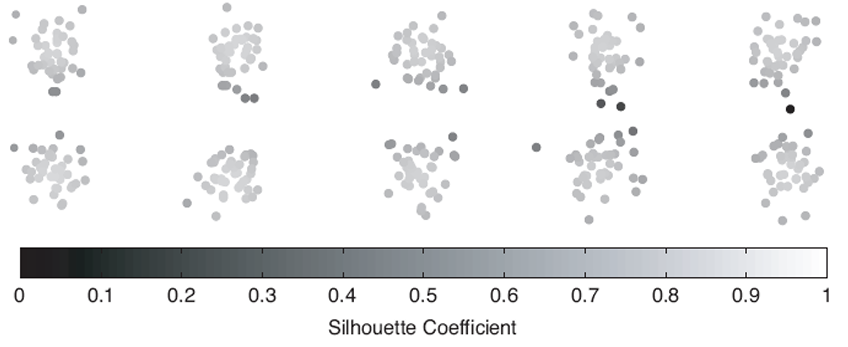
\includegraphics[scale=0.5]{images/silhouette.PNG}
    \caption{A dataset of 10 clusters, with each point $p$ colored by its \textbf{Silhouette Coefficient}: $s = 1 - \frac{a}{b}$ (if $a < b$; otherwise $s = \frac{b}{a} - 1$), with $a$ being the average distance of $p$ to the points in its cluster, and $b$ being the average distance of $p$ to the points outside its cluster. Instances closest to the borders of the clusters have the smallest silhouette coefficient.}
\end{figure}

\begin{figure}[h]
    \centering
    \begin{subfigure}{.5\textwidth}
        \centering
        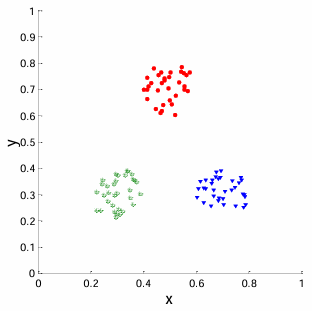
\includegraphics[width=.5\linewidth]{images/cluster-sim1.PNG}
        \caption{Clusters with $corr = 0.9235$.\label{fig:cluster-sim1}}
    \end{subfigure}%
    \begin{subfigure}{.5\textwidth}
        \centering
        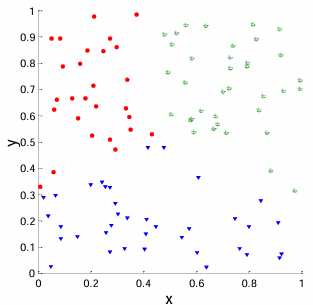
\includegraphics[width=.5\linewidth]{images/cluster-sim2.PNG}
        \caption{Clusters with $corr = 0.5810$.\label{fig:cluster-sim2}}
    \end{subfigure}
\caption{Another unsupervised approach is to use the \textit{similarity} matrix ($n \times n$, with entry $i,j$ being the similarity of points $i$ and $j$) and the \textit{clustering} matrix ($n \times n$, with entry $i, j$ being 1 if and only if points $i$ and $j$ belong to the same cluster): compute the correlation between the two matrices, high correlation indicates that points belonging to the same cluster are close to each other.}
\end{figure}

\begin{figure}[h!]
    \centering
    \begin{subfigure}{.5\textwidth}
        \centering
        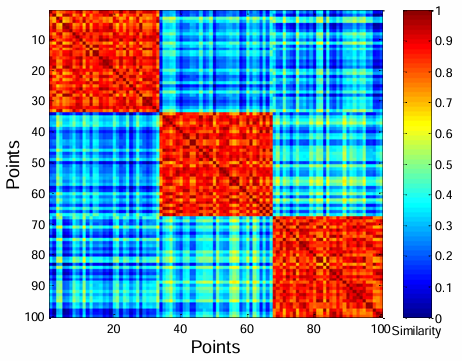
\includegraphics[width=.6\linewidth]{images/simmatrix2.PNG}
        \caption{Similarity matrix for Figure \ref{fig:cluster-sim1}.}
    \end{subfigure}%
    \begin{subfigure}{.5\textwidth}
        \centering
        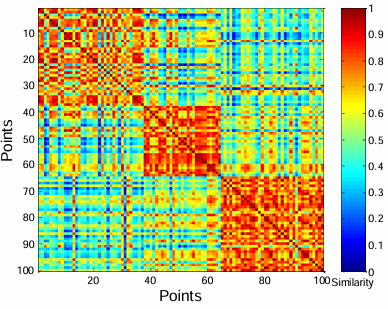
\includegraphics[width=.6\linewidth]{images/simmatrix3.PNG}
        \caption{Similarity matrix for Figure \ref{fig:cluster-sim2}.}
    \end{subfigure}
\caption{Clusters can also be validated using only the similarity matrix and inspecting visually.}
\end{figure}

\newpage
\noindent
For \textit{hierarchical} clusters, the \textbf{Cophenetic Distance} between two objects is the height of the node in the dendogram that represents the first cluster that contains both objects. The \textbf{Cophenetic Correlation Coefficient} is the correlation between the \textit{cophenetic distance} matrix and the \textit{dissimilarity} matrix.

\begin{figure}[h]
    \centering
    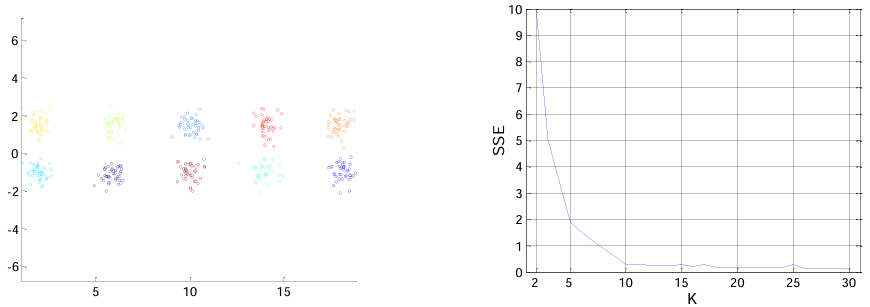
\includegraphics[scale=0.75]{images/elbow-rule.PNG}
    \caption{A big problem with K-means is how to determine the optimal number of clusters $k$. One common technique is the \textbf{Elbow Rule}: calculate the SSE (sum of squared distances from each point to its cluster's centroid) for multiple values of $k$, then inspect the plot for an \textit{elbow} (sudden change in SSE), this is likely the best value for $k$ (in the above example either 5 or 10 works).}
\end{figure}

\noindent
Another way to determine the optimal $k$ is to use \textit{cross-validation}: divide the dataset into $m$ partitions, use $m - 1$ partitions to obtain a clustering model, and calculate the SSE for the remaining test partition.
Repeat this $m$ times for multiple values of $k$ to identify the best fit.

\noindent
\\
In the case that there do exist labels for the clusters, validation can be done using techniques such as \textit{entropy} ($e = \sum_{i = 1}^k \frac{m_i}{n} e_j$, where $k$ is the number of clusters, $n$ is the total number of data points, $m_i$ is the size of cluster $i$, and $e_j = \sum_{i = 0}^L p_{ij} \log_2 p_{ij}$, where $L$ is the total number of classes, and $p_{ij} = \frac{m_{ij}}{m_j}$ is the probability that a member of cluster $j$ belongs to class $i$), \textit{purity} ($pur = \sum_{i = 1}^k \frac{m_i}{n} pur_i$, where $pur_i = \max p_{ij}$), or \textit{similarity} (compute the correlation between the clustering matrix and the true class matrix).

%
% Topic 9 - Association Rule Mining
%
\newpage
\section{Association Rule Mining}
Given a set of \textit{transactions}, the goal of \textbf{Association Rule Mining} is to find \textit{rules} (e.g. $A \rightarrow B$) that can predict occurrences of items based on the occurrences of other items (see Figure \ref{fig:association-rule-mining}).

\noindent
\\
A collection of one or more items is called an \textbf{Itemset} (e.g. $\{ a, b, c \}$).
The \textbf{Support Count} $\sigma(l)$ of an itemset $l$ is the number of times that $l$ appears in the set of transactions (including as a subset).
The \textbf{Support} $s(l)$ of an itemset $l$ is the support count of that itemset over the total number of transactions.
An itemset whose support is greater than or equal to a threshold $t$ is called a \textbf{Frequent Itemset}.
An implication expression of the form $A \rightarrow B$, where $A$ and $B$ are both itemsets, is called an \textbf{Association Rule}.
Association rules of the form $X: A \rightarrow B$ can be evaluated using their \textit{support} $s(X) = s(A + B)$ (also known as \textit{cover}), or \textbf{Confidence} $c(X) = \frac{\sigma(A + B)}{\sigma(A)}$.

\noindent
\\
Given a set of transactions $T$, the goal of association rule mining is to find all rules having $s \geq t_s$ and $c \geq t_c$.
The total number of possible rules is $3^{|T|} - 2^{|T|+1} + 1$, meaning a brute-force approach becomes computationally intractable very quickly.

\subsection{Apriori Algorithm}
Because of the way \textit{support} and \textit{confidence} are defined, rules that cover the same itemset but in a different order (e.g. $ab \rightarrow c$, $a \rightarrow bc$, $c \rightarrow ab$; etc.) have identical \textit{support}, but can have different \textit{confidence}.
This means we can decompose the process of finding rules into a two-step process:

\begin{enumerate}
    \item \textbf{Frequent Itemset Generation}: generate all itemsets whose support $\geq t_s$.
    \item \textbf{Rule Generation}: generate high confidence rules by binary-partitioning the frequent itemsets.
\end{enumerate}

\subsubsection{Frequent Itemset Generation}
Despite this optimization, frequent itemset generation still runs in $O(2^n)$.
A way to further speed this up is using the \textbf{Apriori Principle}: if an itemset is frequent, then all its subsets must also be frequent (conversely; if an itemset is \textit{not} frequent, then all its subsets must also not be frequent):
\[ \forall A, B : (A \subseteq B) \implies s(A) \geq s(B) \]

\begin{figure}[h!]
    \centering
    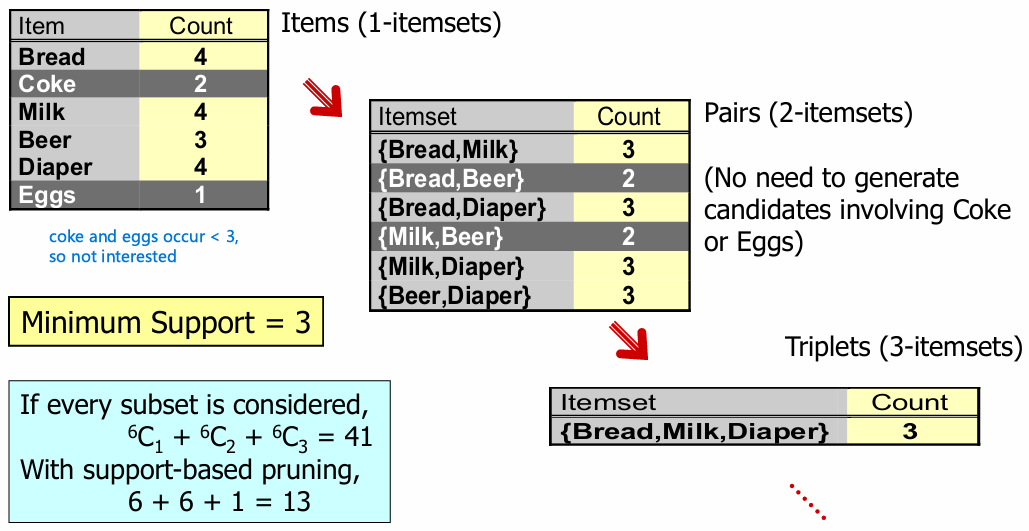
\includegraphics[scale=0.5]{images/apriori-principle.PNG}
    \caption{An example showing how the Apriori principle reduces the "seen" itemsets from 41 to 13.}
\end{figure}

\newpage
\noindent
The \textbf{Apriori Algorithm} for generating frequent itemsets works as follows:

\begin{enumerate}
    \item Let $k = 1$, generate all frequent itemsets of length 1.
    \item Generate length $k + 1$ \textit{candidate} itemsets from length $k$ frequent itemsets.
    \item Prune candidate itemsets containing subsets of length $k$ that are \textit{infrequent}.
    \item Compute the support of the remaining candidate itemsets, prune those that are infrequent.
    \item Repeat from 2. until no new frequent itemsets are identified.
\end{enumerate}

\noindent
The generation of candidate itemsets is done by merging itemsets from the previous generation, for example: if given $L_3 = \{ abc, abd, acd, ace, bcd \}$, $C_4 = \{ abcd, acde \}$, after which $acde$ gets pruned since $ade \notin L_3$.

\subsubsection{Rule Generation}
Given a frequent itemset $L$, rule generation aims to find all non-empty subsets $l \subset L$ such that $c(l \rightarrow L - l) \geq t_c$.
Brute-forcing this gives us $2^|L| - 2$ \textit{candidate} association rules.

\noindent
\\
Unlike \textit{support}, \textit{confidence} does not have the \textit{anti-monotonic} property (i.e. the Apriori principle).
However, the confidence of rules generated from the same itemset \textit{does} have an anti-monotonic property with respect to the number of items on the right-hand side (proof in Appendix \ref{app:math}):
\[ L = \{ a, b, c, d \} \implies c(abc \rightarrow d) \geq c(ab \rightarrow cd) \geq c(a \rightarrow bcd) \]

\noindent
Other factors influencing the complexity of the Apriori algorithm include the choice of $t_s$ (lower threshold means more frequent itemsets), the dimensionality of the dataset (horizontally for computing support count, vertically for multiple passes), and the average transaction width (longer transactions means longer frequent itemsets).

\noindent
\\
Additional ways to speed up the Apriori algorithm include \textit{partitioning} (if the set of transactions $T$ is too big to fit in memory, divide $T$ into $n$ partitions, find the frequent itemsets local to each partition, combine all local frequent itemsets to form the candidate itemsets), \textit{transaction reduction} (a transaction that does not contain any frequent $k$-itemset will also not contain any frequent $k+1$-itemsets, it can therefore be ignored in future scans), and \textit{sampling} (usually with a lower $t_s$ to compensate).

\subsubsection{Compact Itemset Representations}
The number of frequent itemsets generated by the Apriori algorithm can often be very large.
\textbf{Maximal Frequent Itemsets} can form a small representative set from which every frequent itemset can be derived.
An itemset is \textit{maximal frequent} if it is frequent and none of its immediate supersets is frequent (e.g. if $ad$ is frequent, but $abd$ and $acd$ are not frequent, then $ad$ is maximal frequent).
We can obtain all frequent itemsets by \textit{enumerating} over the maximal frequent itemsets (e.g. if $abc$ is maximal frequent, then $a$, $b$, $c$, $ab$, $ac$, $bc$, and $abc$ are all frequent itemsets).

\noindent
\\
An (frequent) itemset is \textbf{Closed} (frequent) if none of its immediate supersets has the same support.
The set of \textit{maximal frequent} itemsets is a subset of the set of \textit{closed frequent} itemsets.

\newpage
\begin{figure}[h]
    \centering
    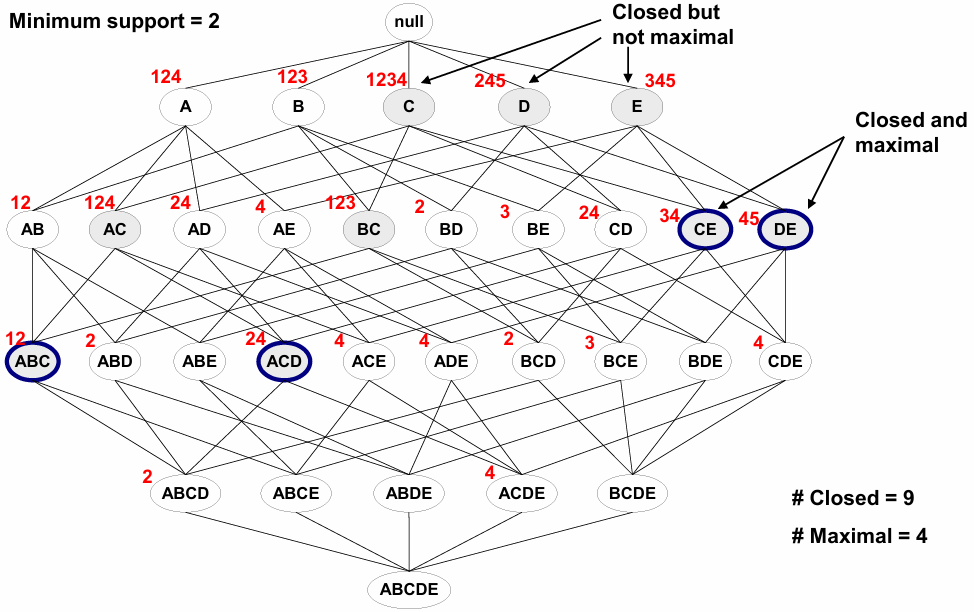
\includegraphics[scale=0.5]{images/max-closed-itemsets.PNG}
    \caption{An example showing the difference between \textit{maximal} and \textit{closed} frequent itemsets. The red numbers show the transaction IDs of the following transaction set: $\{ ABC, ABCD, BCE, ACDE, DE \}$ (e.g. $A^{124}$ means there is support in transaction IDs 1, 2 and 4, so $\sigma(A) = 3$).}
\end{figure}

\noindent
The transaction set can also be made more compact using a \textit{vertical} data layout: instead of storing the items for each transaction ID, store the transaction IDs for each item:
\begin{align*}
    \begin{tabular}{|c|c|}
    \hline
    \text{IDs} & \text{Items} \\ \hline
    1 & A, B, E \\
    2 & B, C, D \\
    3 & C, E \\
    ... & ... \\ \hline
    \end{tabular} && \longrightarrow &&
    \begin{tabular}{|c|c|c|c|}
    \hline
    A & B & C & ... \\ \hline
    1 & 1 & 2 & ... \\
    4 & 2 & 3 & ... \\
    5 & 5 & 4 & ... \\
    ... & ... & ... & ... \\ \hline
    \end{tabular}
\end{align*}

\noindent
Support for any $k$-itemset can be very efficiently computed by intersecting its columns (e.g. $AB$: $A \wedge B = $ IDs 1, 5, ...).

\subsection{Quality Measures for Association Rules}
The confidence of $A \rightarrow B$ is equal to the probability of observing $B$, given that you have already observed $A$: $P(B | A)$.
The problem with using \textit{confidence} to measure the quality of rules is that when $B$ is independent of $A$: $P(B | A) = P(B)$.
If $P(B)$ is high, then $A \rightarrow B$ will have a high confidence despite $A$ and $B$ being independent.
The \textbf{Lift} measure indicates the (in)dependence of $A$ and $B$:
\[ lift(A \rightarrow B) = \frac{c(A \rightarrow B)}{P(B)} = \frac{P(A \wedge B)}{P(A) P(B)} \]

\noindent
The lift is 1 when $A$ and $B$ are independent, greater than 1 if there is a \textit{positive} correlation (i.e. $A$ implies the occurrence of $B$), or less than 1 if there is a \textit{negative} correlation (i.e. $A$ implies the absence of $B$; in this case the rule is very bad).
The big problem of lift is that it is \textit{symmetric}: it does not take the direction of the implication into account.
A measure that takes the direction of the implication, as well as a possible independence is \textbf{Conviction} ($[0, \infty]$, 1 if independent):
\[ conv(A \rightarrow B) = \frac{P(A) P(\lnot B)}{P(A \wedge \lnot B)} \]

\newpage
\subsection{Frequent Pattern Growth Algorithm}
The \textbf{Frequent Pattern Growth (FP-Growth)} algorithm mines frequent itemsets from large transaction sets. Unlike the Apriori algorithm, which suffers from high computational cost due to candidate generation and multiple database scans, FP-Growth avoids these inefficiencies by compressing the data into an \textbf{Frequent Pattern Tree (FP-Tree)} and extracts patterns directly from it.
The complexity of the FP-Growth algorithm depends very much on the \textit{compactness} of the data.

\begin{figure}[h]
    \centering
    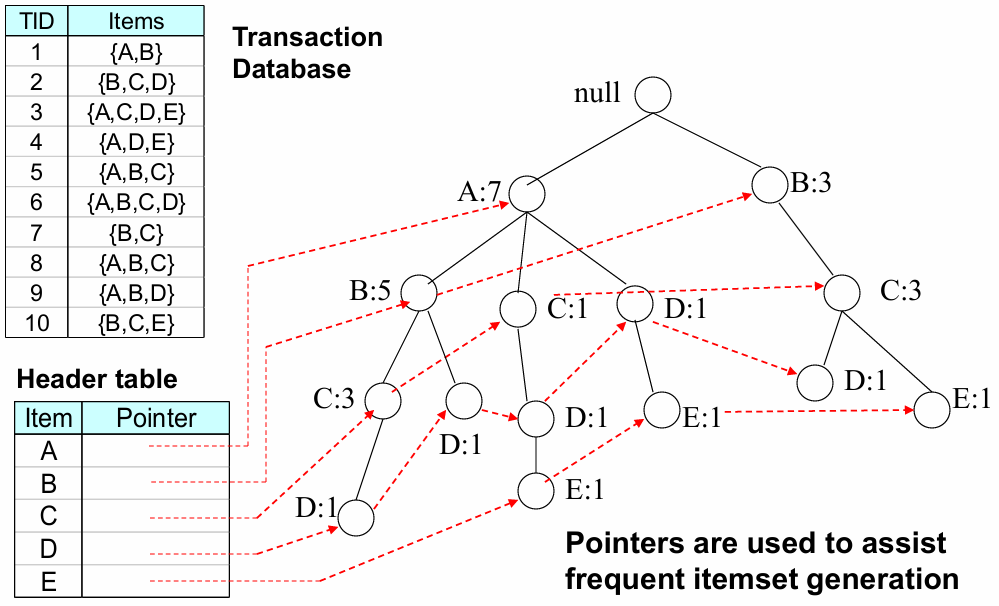
\includegraphics[scale=0.5]{images/fp-tree.PNG}
    \caption{An FP-Tree constructed from a transaction set.}
\end{figure}

\subsection{Categorical and Numerical Data}
By incorporating categorical and numerical data we can create more complex rules, for example:
\[ \{ \text{Number of Page} \in [5, 10] \wedge (\text{Browser} = \text{Firefox}) \} \rightarrow (\text{Buy} = \text{No}) \]

\noindent
\textit{Categorical} attributes can be transformed into asymmetric binary variables through \textbf{One-Hot Encoding}.
This has possible issues such as an attribute having many possible values, or the distribution being skewed in one value's favour (possibly ignore values that have \textit{too low} or \textit{too high} support).

\noindent
\\
\textit{continuous} attributes can be used through \textbf{Discretization-Based Handling} (equal-width binning, equal-depth binning, clustering, etc.), or \textbf{Statistics-Based Handling}:

\begin{enumerate}
    \item Withhold the target attribute from the rest of the data, extract frequent itemsets.
    \item Each frequent itemset becomes the left-hand side of a rule, with the right-hand side being the corresponding value of the target attribute (e.g. $\{ \text{income} > 100k \} \rightarrow \{ \mu_\text{age} = 34 \}$).
    \item Apply a statistical test to determine the "interestingness" of the rule (compare the population covered by the rule vs. the population not covered: $A \rightarrow B: \mu$ vs. $\bar{A} \rightarrow B: \mu^\prime$; Null hypothesis $\mu^\prime = \mu + \Delta$ ($\Delta$ is the "acceptable" range, e.g. 5 years); Alternative hypothesis: $\mu^\prime > \mu + \Delta$; $Z = (\mu^\prime - \mu - \Delta) / \sqrt{\frac{\sigma_1^2}{n_1} + \frac{\sigma_2^2}{n_2}}$, where $n_1$ is the number of samples and $\sigma_1$ is the standard deviation of $B$ that support $A$; Under the null hypothesis, $\mu_Z = 0$, $\sigma_Z^2 = 1$; At 95\% confidence level, a rule is interesting if $Z > 1.64$).
\end{enumerate}

%
% Appendix
%
\newpage
\appendix
\section{Mathematical Derivations} \label{app:math}

\begin{figure}[h]
    \centering
    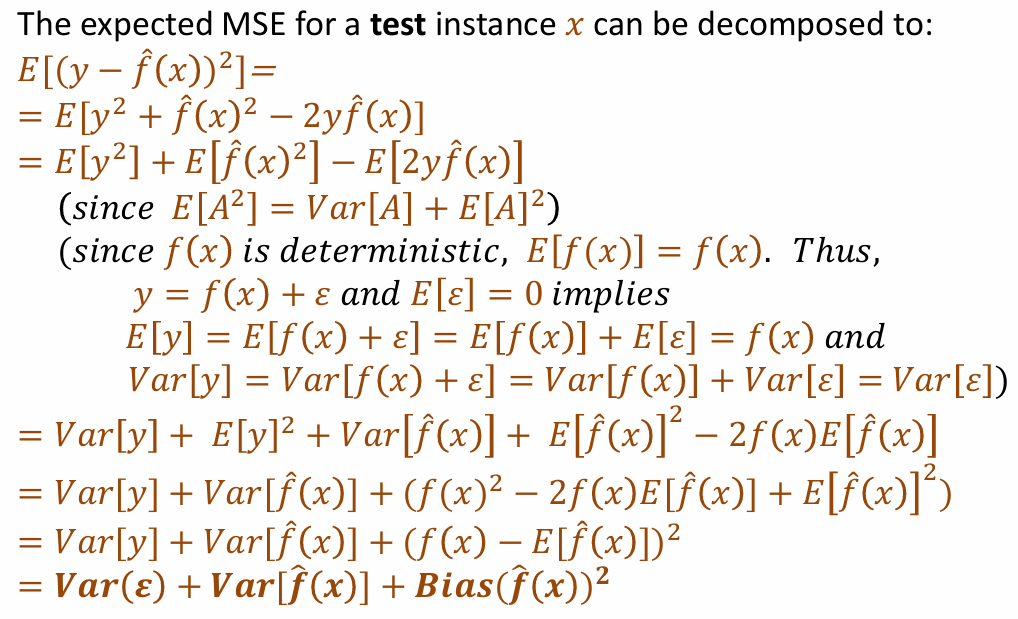
\includegraphics[scale=0.75]{images/bias-variance-tradeoff.PNG}
    \caption{Full derivation of the \textbf{Bias-Variance Tradeoff}.}
\end{figure}

\begin{figure}[h!]
    \centering
    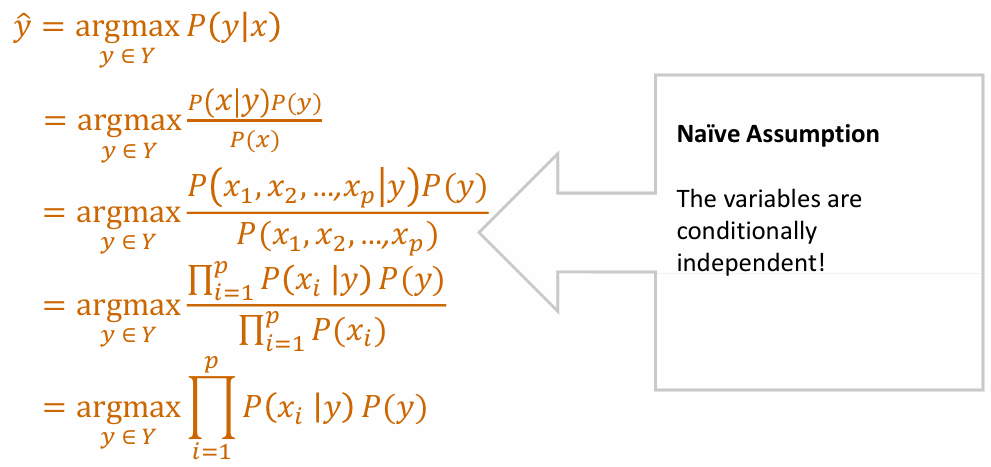
\includegraphics[scale=0.75]{images/naive-bayes.PNG}
    \caption{Full derivation of the \textbf{Naive Bayes Classifier}.}
\end{figure}

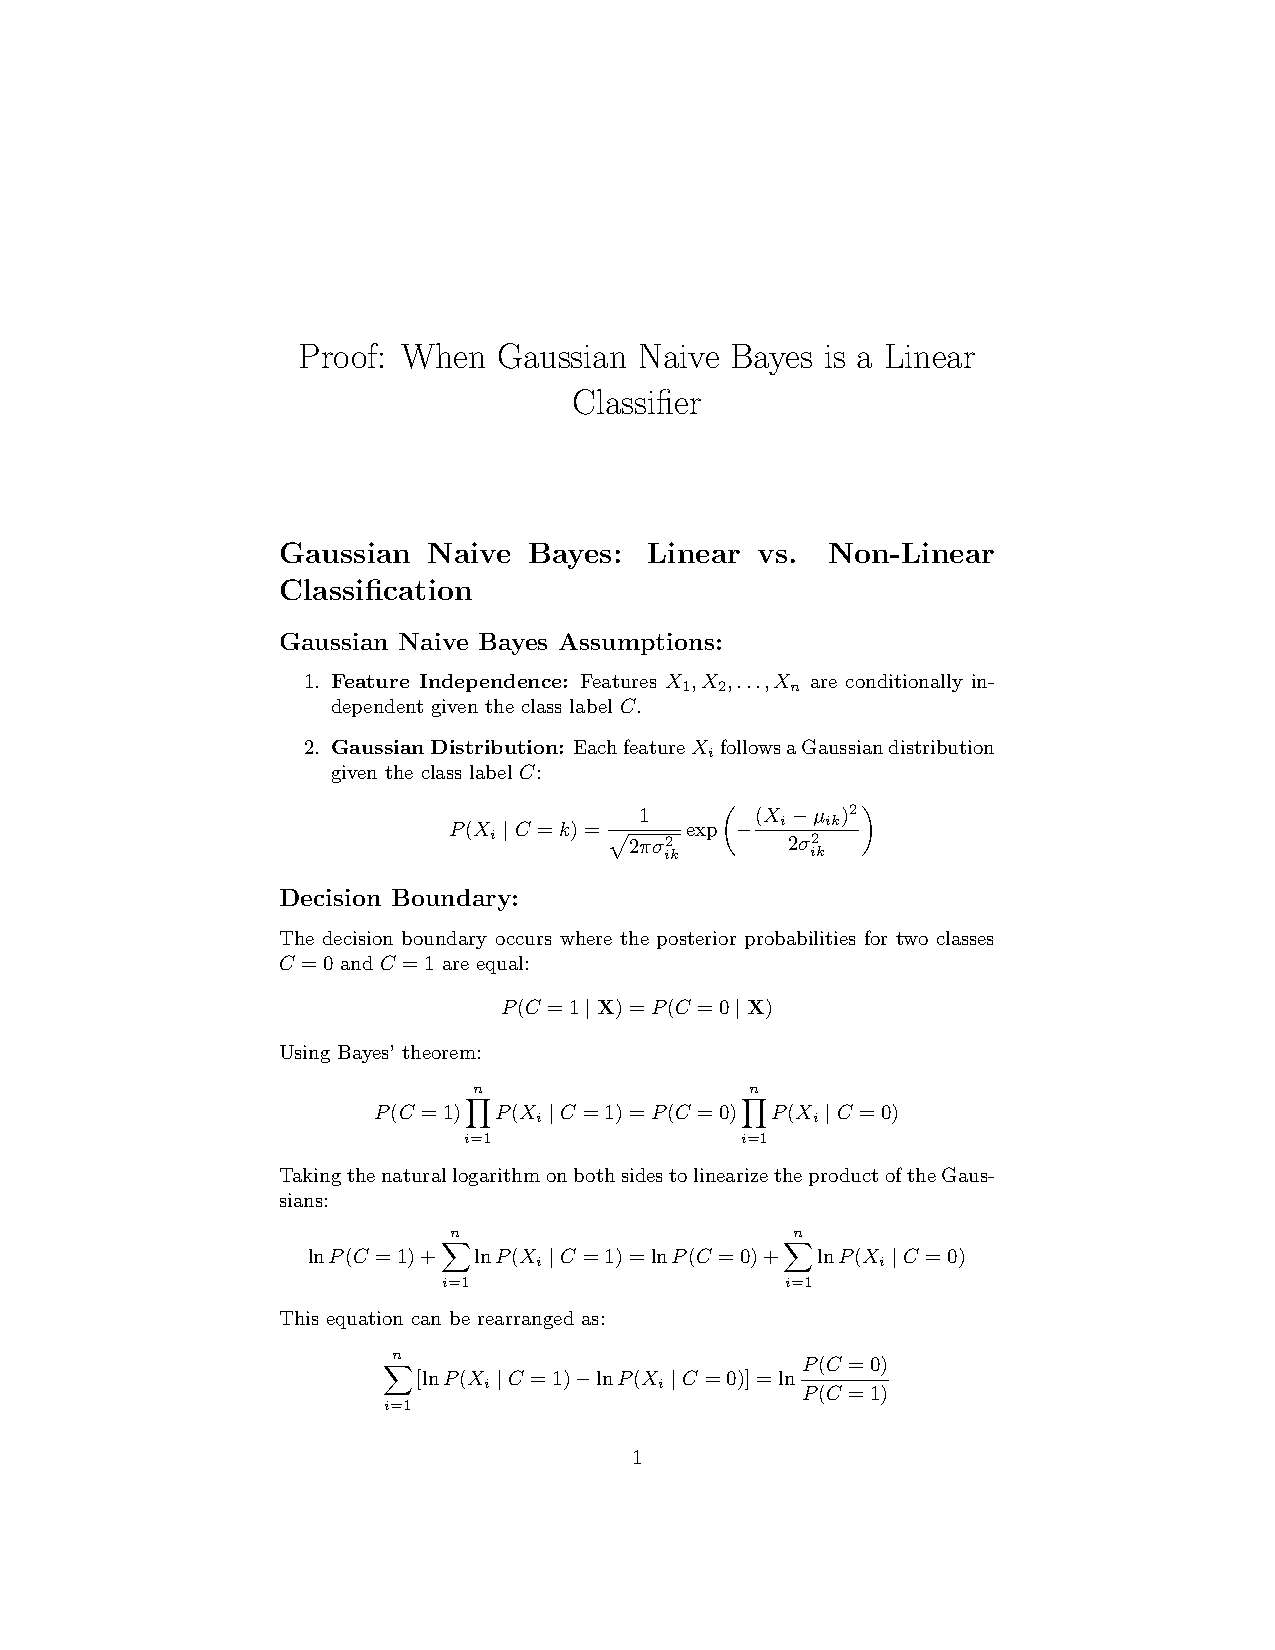
\includepdf[pages=-]{images/naive-bayes-linearity.pdf}

\begin{figure}[h]
    \centering
    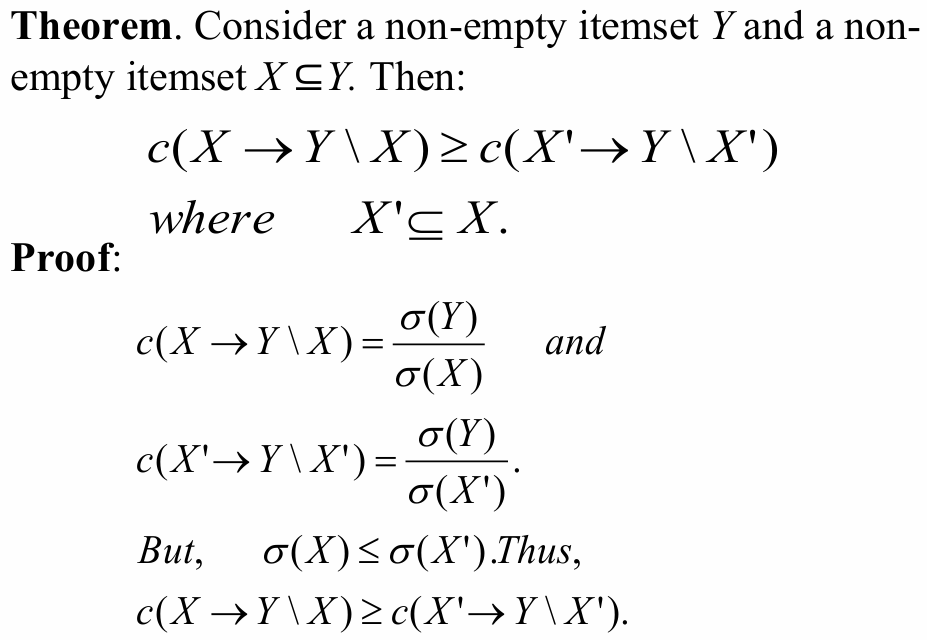
\includegraphics[scale=0.75]{images/conf-nonmono.PNG}
    \caption{Proof of the non-monotonic property of \textbf{Confidence}.}
\end{figure}

\newpage
\section{Additional Content}
\subsection{Confidence Intervals} \label{app:conf}
Assume that the estimated accuracy $acc_S(h)$ of classifier $h$ is $75\%$ on a dataset $S$.
How close is $acc_S(h)$ to the true accuracy $acc_D(h)$ over the whole data distribution $D$?
The classification of an instance is a Bernoulli trail with two outcomes: \textit{correct} and \textit{incorrect}.
The random variable $X$, representing the number of correct trials over $N$ classifications, has a Binomial distribution $B(N, acc_D)$ with mean $N \cdot acc_D$ and variance $N \cdot acc_D (1 - acc_D)$.
It can be shown that the empirical accuracy $acc_S = \frac{X}{N}$ also follows a Binomial distribution with mean $acc_D$ and variance $\frac{acc_D (1 - acc_D)}{N}$.
For large test sets ($N > 30$), we can approximate this Binomial distribution by a Normal distribution with mean $acc_D$ and variance $\frac{acc_D (1 - acc_D)}{N}$.
Thus, with lower bound $Z_{\alpha / 2}$ and upper bound $Z_{1 - \alpha / 2}$:
\[ P \left( Z_{\alpha / 2} < \frac{acc_S - acc_D}{\sqrt{\frac{acc_D (1 - acc_D)}{N}}} < Z_{1 - \alpha / 2} \right) = 1 - \alpha \]

\noindent
The confidence interval for $acc_D$ is given by:
\[ \frac{2N \cdot acc_S + Z_{\alpha / 2}^2 \pm \sqrt{Z_{\alpha / 2}^2 + 4N \cdot acc_S - 4N \cdot acc_S^2}}{2 \left( N + Z_{\alpha / 2}^2 \right)} \]

\noindent
The confidence intervals shrink when we decrease confidence:

\begin{table}[h]
    \centering
    \begin{tabular}{c|ccccccc}
    $1 - \alpha$ & 0.99 & 0.98 & 0.95 & 0.9 & 0.8 & 0.7 & 0.5 \\ \hline
    $Z_{\alpha / 2}$ & 2.58 & 2.33 & 1.96 & 1.65 & 1.28 & 1.04 & 0.67
    \end{tabular}
\end{table}

\noindent
The confidence intervals become tighter when the number of test instances $N$ increases:

\begin{table}[h]
    \centering
    \begin{tabular}{c|cccccc}
    $N$ & 20 & 50 & 100 & 500 & 1000 & 5000 \\ \hline
    $CI$ ($\alpha = 0.05$) & [0.58, 0.92] & [0.67, 0.89] & [0.71, 0.87] & [0.76, 0.83] & [0.77, 0.82] & [0.78, 0.81]
    \end{tabular}
\end{table}

\noindent
Now assume that we have two classifiers $h_1$ and $h_2$, and we would like to know which one is better.
We test the classifiers on $m$ test sets and receive error rate estimates $e_{11}, e_{12}, ... , e_{1n}$ for classifier $h_1$ and $e_{21}, e_{22}, ... , e_{2n}$ for classifier $h_2$.
We consider the differences $d_1, d_2, ... , d_n$ with $d_j = |e_{1j} - e_{2j}|$.
These differences are instantiations of $n$ random variables $D_1, D_2, ... , D_n$ with mean $\mu_D$ and standard deviation $\sigma_D$.
We need to establish confidence intervals for $\mu_D$ to decide whether the difference in performance between $h_1$ and $h_2$ is statistically significant or not.
Since $\sigma_D$ is unknown, we estimate it using the sample standard deviation:
\[ s_d = \sqrt{\frac{1}{n} \sum_{i = 1}^n \left( \left( e_{1i} - e_{2i} \right) - \left( \bar{e}_1 - \bar{e}_2 \right) \right)} \]

\noindent
We introduce a $T$-statistic governed by a $t$-distribution with $n-1$ degrees of freedom: if $\bar{d}$ and $s_d$ are the mean and standard deviation of the normally distributed differences of $n$ random pairs of errors, a $(1 - \alpha)100\%$ confidence interval for $\mu_D = \mu_1 - \mu_2$ is given by:
\[ \bar{d} - t_{\alpha / 2} \frac{s_d}{\sqrt{n}} < \mu_D < \bar{d} + t_{\alpha / 2} \frac{s_d}{\sqrt{n}} \]

\noindent
Where $t_{\alpha / 2}$ is the $t$-value with $v = n - 1$ degrees of freedom.

\subsection{Model-Based Clustering}
\begin{figure}[h]
    \centering
    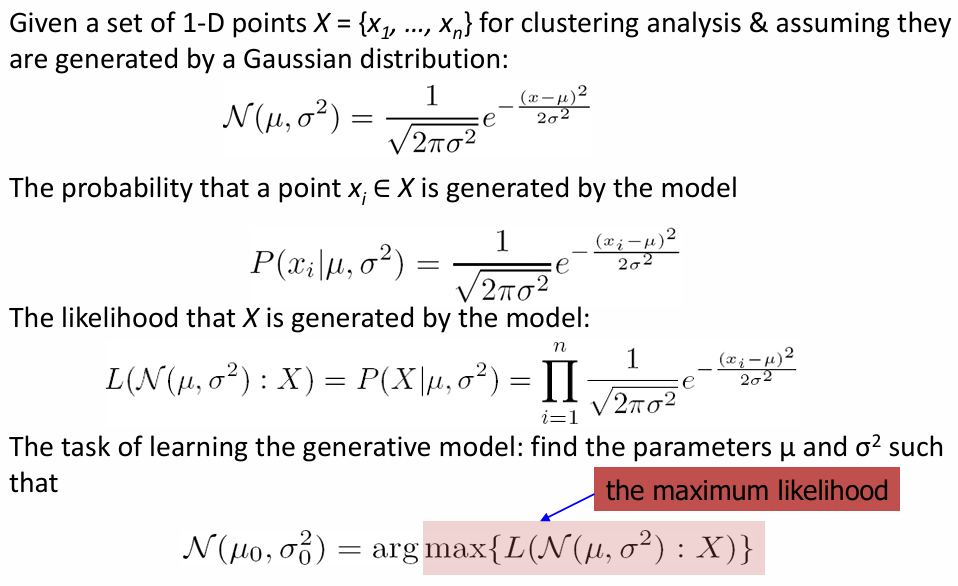
\includegraphics[scale=0.5]{images/modelcluster1.PNG}
    \caption{Generative models for model-based clustering.}
\end{figure}

\begin{figure}[h]
    \centering
    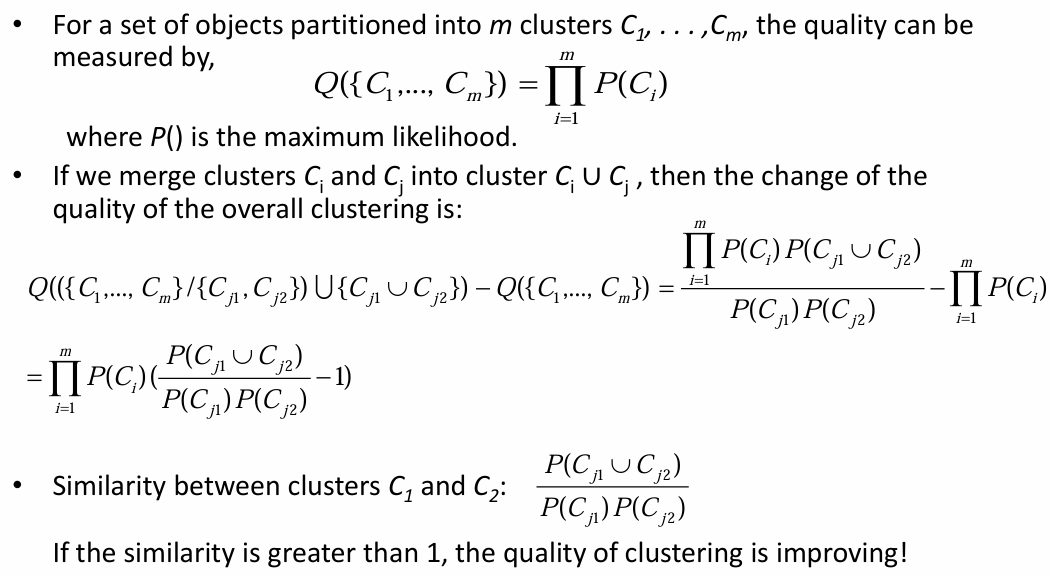
\includegraphics[scale=0.5]{images/modelcluster2.PNG}
    \caption{A probabilistic hierarchical clustering algorithm.}
\end{figure}

\begin{figure}[h!]
    \centering
    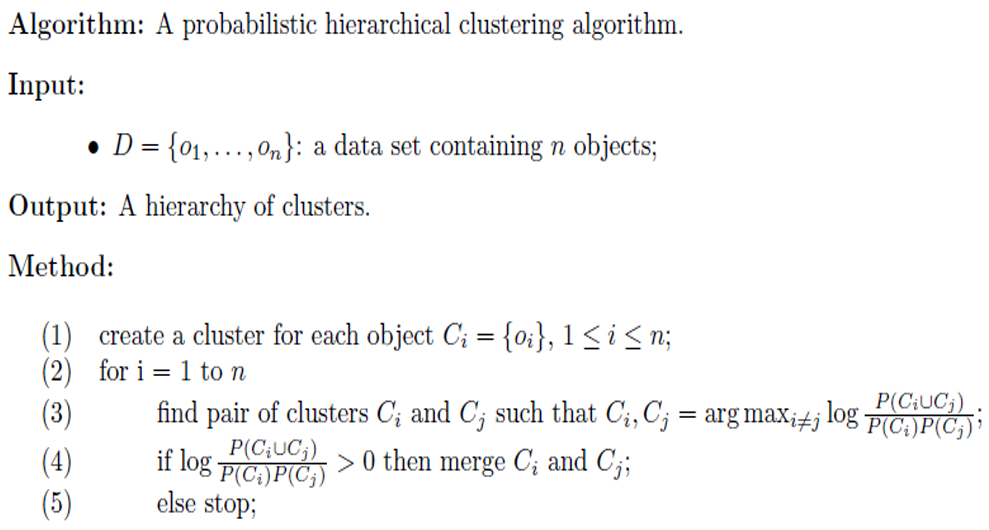
\includegraphics[scale=0.5]{images/modelcluster3.PNG}
    \caption{Pseudocode for a probabilistic hierarchical clustering algorithm.}
\end{figure}

\begin{figure}[h]
    \centering
    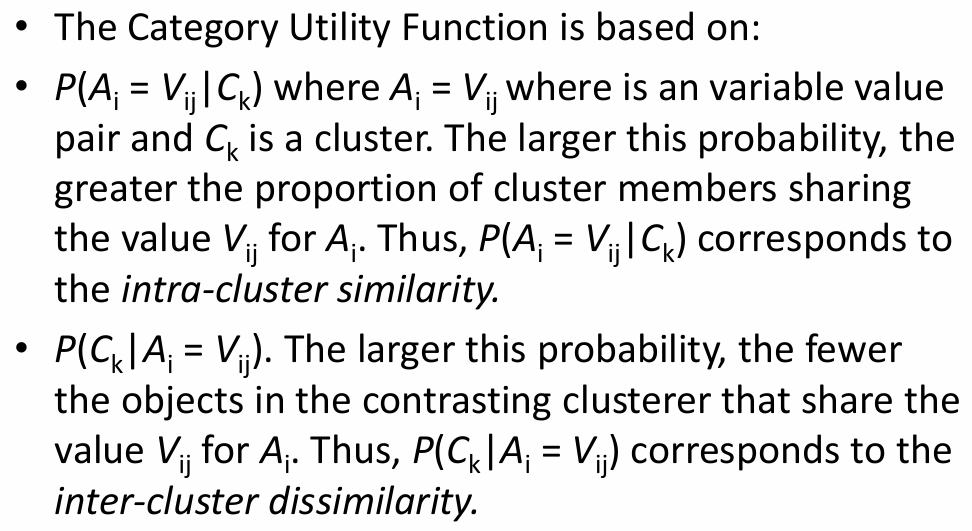
\includegraphics[scale=0.5]{images/modelcluster4.PNG}
\end{figure}

\begin{figure}[h]
    \centering
    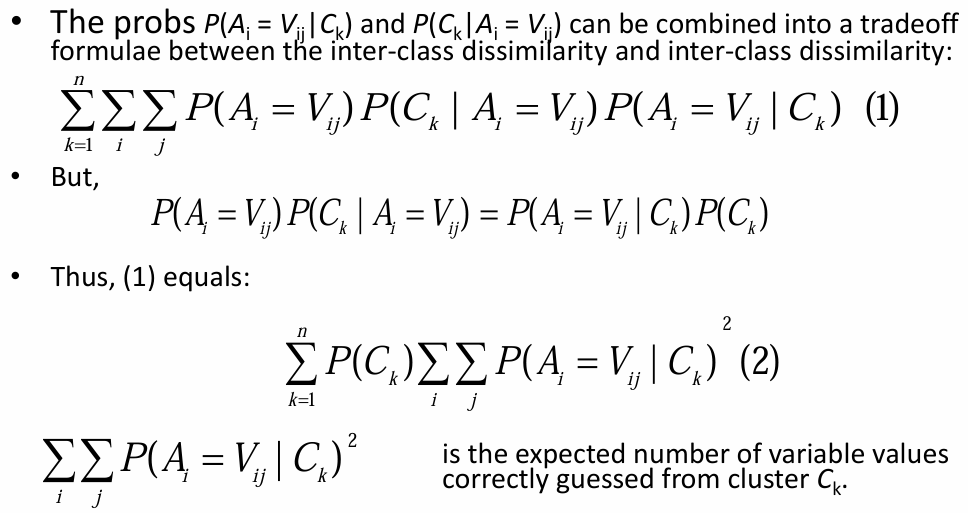
\includegraphics[scale=0.5]{images/modelcluster5.PNG}
\end{figure}

\begin{figure}[h!]
    \centering
    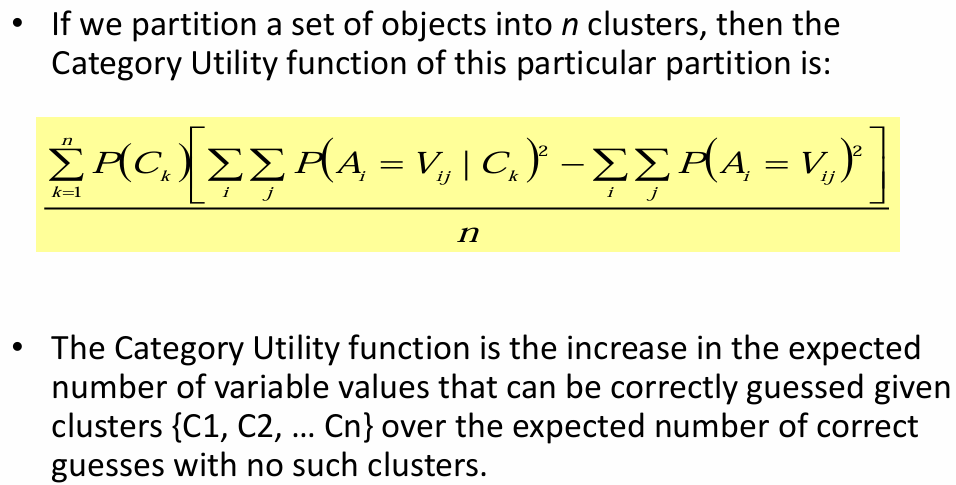
\includegraphics[scale=0.5]{images/modelcluster6.PNG}
    \caption{The Category Utility Function.}
\end{figure}

\end{document}
